\documentclass[a4paper,12pt,twoside]{article}%twoside
\usepackage[utf8]{inputenc}
\usepackage[dutch]{babel}
\usepackage{fancyhdr, amsmath, color, graphicx, enumitem, tabularx, hyperref, longtable, multirow, placeins, apacite, subcaption,marvosym,multicol}
\usepackage[framemethod=tikz]{mdframed}

\usepackage[europeanresistors,americaninductors,americancurrents,siunitx]{circuitikz}

\usepackage[margin=2.5cm,headheight=68pt]{geometry}
%\usepackage[total={16cm, 22cm}]{geometry}

\pagestyle{fancy}
\fancyhf{}
\fancyhead[LE,RO]{Specifieke Lerarenopleiding voor CVO-studenten}%'E': even page, 'O': odd page
\fancyhead[RE,LO]{Didactische Competentie Stage}
\fancyfoot[RE,CO]{}
\fancyfoot[LE,RO]{KU Leuven campus Kortrijk Kulak   \thepage}
%\renewcommand{\labelitemi}{$\circ$}

\definecolor{CVO}{RGB}{232, 0, 97}
\setlength\parindent{0pt}
\title{Stageportfolio}
\author{Kevin Truyaert}
\date{}


% %FOOTER IN MDFRAMED
\usepackage{footnote} 
\newenvironment{mdframedwithfoot}
{   
	\savenotes
	\begin{mdframed}
		\stepcounter{footnote}
		\renewcommand{\thefootnote}{\arabic{footnote}}
	}
	{
	\end{mdframed}
	\spewnotes
}


%FOOTER IN PARBOX
\makeatletter
\newcommand{\global@insert}[2]% #1=box number, #2=vertical list
{\bgroup
	\setbox\@tempboxa=\box#1
	\global\setbox#1=\vbox{\unvbox\@tempboxa #2}
	\egroup}

\long\def\@footnotetext#1{\global@insert\footins{%
		\reset@font\footnotesize
		\interlinepenalty\interfootnotelinepenalty
		\splittopskip\footnotesep
		\splitmaxdepth \dp\strutbox \floatingpenalty \@MM
		\hsize\columnwidth \@parboxrestore
		\protected@edef\@currentlabel{%
			\csname p@footnote\endcsname\@thefnmark
		}%
		\color@begingroup
		\@makefntext{%
			\rule\z@\footnotesep\ignorespaces#1\@finalstrut\strutbox}%
		\color@endgroup}}%
\makeatother
%%%%%%%%%%%%%%%%%%%%%%%%%

%Strikeout and highlight text
\usepackage{soul}
\usepackage{tikz} % only to get \foreach

%\definecolor{yellow}{RGB}{255,255,0}
\sethlcolor{yellow}

% \newcommand*{\YellowHighlight}[1]{{\hl{~#1~}}}
\newcommand*{\PinkHighlight}[2]{{\hspace{-1.5mm}\colorbox{pink}{\parbox{#2}{~#1~}}}}
\newcommand*{\GreenHighlight}[2]{{\hspace{-1.5mm}\colorbox{green}{\parbox{#2}{~#1~}}}}
\newcommand*{\YellowHighlight}[2]{{\hspace{-1.5mm}\colorbox{yellow}{\parbox{#2}{~#1~}}}}
% % % % % %

\usepackage{tabularx,pdflscape,pdfpages}

\newcolumntype{C}[1]{>{\centering\let\newline\\\arraybackslash\hspace{0pt}}m{#1}}
\newcolumntype{Q}[1]{>{\flushleft\let\newline\\\arraybackslash\hspace{0pt}}p{#1}}

\begin{document}
	\maketitle
	
	
	\section*{Identificatiegegevens}
	\begin{center}
		\begin{tabular}{ll}
			\hline
			Naam: & Kevin Truyaert\\ \hline
			Adres: & Bolle-Akkerweg 4\\
			& 8800 Roeselare\\\hline
			Telefoon: & 0032495/928460\\\hline
			Mail: & kevin.truyaert@student.kuleuven.be\\\hline
			Naam stagebegeleider: & Cato De Baets\\ \hline
		\end{tabular}
	\end{center}
	
	\newpage
	\tableofcontents
	\newpage
	
	
	% !TeX root = Stageportfolio.tex

\begin{landscape}
\section{Observatie- en stageplanning}

\subsection{Observatieplanning}

\begin{tabularx}{1.56\textwidth}{|C{0.15\textwidth}|C{0.14\textwidth}|C{0.14\textwidth}|C{0.1\textwidth}|C{0.1\textwidth}|C{0.05\textwidth}|C{0.35\textwidth}|X|}
	
	
\end{tabularx}
	

\subsection{Actieve stage}
\begin{table}[]
	\begin{tabularx}{1.56\textwidth}{|X|}
		\hline
		Naam stagair:  Kevin Truyaert  \\
		Tel.: 0495/928460 \hspace{3cm} e-mail: kevin.truyaert@student.kuleuven.be  \\
		Naam en adres opleidingsinstituut:  KU Leuven Campus Kulak Kortrijk, Etienne-Sabbelaan 53, 8800 Kortrijk  \\
		Naam directie: \\
		Naam stagecoördinator:  David Dudal \\
		\hline
	\end{tabularx}
\end{table}
		
	\begin{tabularx}{1.56\textwidth}{|C{0.15\textwidth}|C{0.14\textwidth}|C{0.14\textwidth}|C{0.1\textwidth}|C{0.1\textwidth}|C{0.05\textwidth}|C{0.35\textwidth}|X|}
		\hline
		\textbf{Datum} & \textbf{Vestiging} & \textbf{\begin{tabular}[C]{@{}l@{}}Aantal\\ stage-uren\end{tabular}} & \textbf{\begin{tabular}[C]{@{}l@{}}Uur \end{tabular}}    & \textbf{Lokaal}& \textbf{\begin{tabular}[C]{@{}l@{}}AV\\TV\\PV\\KV\end{tabular}}& \textbf{\begin{tabular}[C]{@{}l@{}}Onderwijsvorm\\ graad en lj\\ Vak en lesonderwerp\end{tabular}}  &  \textbf{\begin{tabular}[C]{@{}l@{}}Naam vakmentor\\ + handtekening\end{tabular} } \\ \hline
		27/11/2019 & Kulak & 1-3 & 10:30-13:00 & A352 & AV & Universiteit\newline 2e jaar Handelsingenieur\newline Conceptuele natuurkunde\newline werkzitting elektromagnetisme & \\ \hline
		4/12/2019 & Kulak & 4-6 & 10:30-13:00 & A352 & AV & Universiteit\newline 2e jaar Handelsingenieur\newline Conceptuele natuurkunde\newline werkzitting elektromagnetisme & \\ \hline
		11/12/2019 & Kulak & 7-9 & 10:30-13:00 & A352 & AV & Universiteit\newline 2e jaar Handelsingenieur\newline Conceptuele natuurkunde\newline werkzitting elektromagnetisme & \\ \hline
	\end{tabularx}
\begin{tabularx}{1.56\textwidth}{|C{0.15\textwidth}|C{0.14\textwidth}|C{0.14\textwidth}|C{0.1\textwidth}|C{0.1\textwidth}|C{0.05\textwidth}|C{0.35\textwidth}|X|}
	\hline
		18/12/2019 & Kulak & 10-12 & 10:30-13:00 & A352 & AV & Universiteit\newline 2e jaar Handelsingenieur\newline Conceptuele natuurkunde\newline werkzitting elektromagnetisme & \\ \hline
		 &  &  &  &  &  &  & \\ \hline
	\end{tabularx}
		


		
\end{landscape}		
		

	
	
	
	% !TeX root = Stageportfolio.tex

\section{Persoonlijk ontwikkelingsplan}
\begin{tabularx}{\textwidth}{|p{0.15\textwidth}|p{0.795\textwidth}|}
	\hline
	\textbf{Lesdoel 1} & 
	\underline{FG 1: de leraar als begeleider van leer- en}\newline \underline{ontwikkelingsprocessen}\newline
	
	1.8 De leraar kan observatie en evaluatie voorbereiden en uitvoeren met het oog op bijsturing en remediëring als onderdeel van het leerproces van een lerende(n) en kan die observatie-en evaluatiegegevens gebruiken om zijn eigen didactische handelen in vraag te stellen en bij te sturen waar nodig.\\ \hline
	Actie 1 & Tijdens het lesgeven wil ik veel in interactie treden. Dit zou ik met zoveel mogelijk leerlingen willen doen en niet steeds dezelfde leerlingen aan bod laten komen. Het lijkt mij uitdagend om dit in realiteit om te zetten. Door hen gerichte vragen te stellen, kan ik kijken waar er mogelijke problemen zijn met de leerstof en van daaruit werken om de lesdoelen begrijpelijk te maken voor alle leerlingen. \\ \hline
	Actie 2 & Na het verbeteren van een taak, een toets of extra oefeningen wil ik die met de leerling(en) overlopen door de meest voorkomende fouten te bespreken. Zo kan ik hen bijsturen en kan ik de belangrijkste punten aanhalen waar er problemen waren. Tegelijkertijd kom ik zo te weten waar ik te weinig nadruk gelegd heb tijdens de les. Hier kan ik nu mee aan de slag om mijn toekomstige lessen aan te passen en om te verhinderen dat hetzelfde soort fouten bij soortgelijke zaken minder gemaakt worden. \\ \hline
\end{tabularx}


\vspace{0.5cm}
\begin{tabularx}{\textwidth}{|p{0.15\textwidth}|p{0.795\textwidth}|}
	\hline
	\textbf{Lesdoel 2} & \underline{FG3: de leraarals inhoudelijk expert} \newline\newline 3.3 De leraar beheerst de kennis en vaardigheden met betrekking tot de (vak)didactiek van zijn onderwijsopdracht. Hij kan die  actualiseren, verbreden en verdiepen. \\ \hline
	Actie 1 & Ik wil als leraar in staat zijn om de theorie interessant over te kunnen brengen. Dit wil ik doen door actuele zaken als voorbeeld van die theorie te gebruiken. Een voorbeeld hiervan: ieder jaar wordt een flitsmarathon aangekondigd. De flitscamera werkt volgens het Dopplereffect. Dus wanneer ik dat moet uitleggen aan de leerlingen, kan ik de flitscamera als voorbeeld gebruiken. Door actuele thema's en alledaagse voorwerpen te linken met fysische verschijnselen, hoop ik dat de leerlingen de wereld rond hen beter begrijpen. \\ \hline
	Actie 2 & Als leerkracht vind ik het belangrijk dat je de leerstof die je aan het bespreken bent, goed begrijpt en dat je de achtergrond ervan ook kent, ook al behandel je die niet in de les. Ik vind dat je als leerkracht de leerstof enkele niveaus dieper moet beheersen dan dat je ze moet overbrengen. Op die manier kan je beter begrijpen vanwaar alles komt en zou je meerdere invalswegen moeten hebben om de te geven leerstof aan je leerlingen over te brengen. \\ \hline
\end{tabularx}


\vspace{0.5cm}
\begin{tabularx}{\textwidth}{|p{0.15\textwidth}|p{0.795\textwidth}|}
	\hline
	\textbf{Lesdoel 3} & \underline{FG5:  de leraar als innovator - de leraar als onderzoeker}\newline\newline
	5.1 De leraar kan de kwaliteit van zijn onderwijs verder ontwikkelen. De leraar kan zijn eigen onderwijspraktijk en zijn eigen functioneren in vraag stellen en bijsturen (verbeteren) door te innoveren om zijn eigen praktijk te verbeteren.\\ \hline
	Actie 1 & Ik verzorg reeds drie jaar oefenzittingen aan de universiteit. Dit jaar wil ik iets nieuws proberen en de studenten actiever de oefeningen laten maken. Ik wil hen in groep aan de oefeningen laten werken, waardoor ze met elkaar in interactie kunnen treden om de oefeningen samen tot een goed eind te kunnen brengen. Op die manier wil ik tijdens mijn oefenzittingen voor innovatie bij lessen in het hoger onderwijs zorgen. \\ \hline
	Actie 2 & Bij de lessen die ik in het middelbaar zal verzorgen, wil ik terugkoppelen naar mijn stagelessen die ik bij DCO deed. Hier gaf ik telkens de introductieles van een nieuw stuk theorie. Die gaf ik relatief `klassiek', waarbij ik als leerkracht veel aan bod kwam. Ik wil nu proberen om de leerlingen zal actiever aan de slag te zetten bij de start van een nieuw stuk. Ik zie dit nu ook meer zitten, omdat ik meer dan één les(blok) per klas zal brengen. Dit zal als gevolg hebben dat ik een groter plan kan uitwerken en zo proberen om mijn eigen lesgeven te innoveren.    \\ \hline
\end{tabularx}
	
	
	\begin{landscape}
		
		\section{Bespreking lesobservaties}
		
		\subsection{Bespreking observatieles 1 Kulak  (LIO)}
		\begin{tabularx}{1.56\textwidth}{|Q{0.25\textwidth}|Q{0.1\textwidth}|Q{0.25\textwidth}|Q{0.85\textwidth}|}\hline
			\textbf{Naam student: Kevin Truyaert} & & Aandachtspunten (o.b.v. POP) & Reflectie:\newline -Wat leerde ik uit mijn observatie over mijn aandachtspunten? \newline -Wat doe ik ermee tijdens mijn stage?\\\hline
			Observatieles 1 \newline \underline{Datum:} 14/11/2019 \underline{Klas:} 2e bachelor Handelsingenieurs \newline \underline{Lesonderwerp:} De wet van Gauss bij geleiders & 1 & Hoe evalueert de prof tijdens de les om te zien of bepaalde lesdoelen tijdens de les bereikt zijn? & Na het zien van een stuk theorie, overloopt de prof samen met de studenten een toepassing op het net geziene stuk theorie. De toepassing wordt door de studenten uitgelegd. De prof stuurt hen door gericht vragen te stellen.  Daarnaast worden de studenten ook bij het zien van de afleiding van nieuwe theorie vaak betrokken. Ze hebben vaak de net geziene onderwerpen nodig om het nieuwe te begrijpen. Ook hier stelt de prof opnieuw gerichte vragen om het antwoord van de leerlingen te krijgen.\newline Ik zie dit als een snelle manier om te polsen of je publiek, of toch een deel ervan, de lesdoelen bereikt heeft. Ik zou echter graag nog een breder gamma aan snelle evaluatietools in mijn bezit krijgen. Tijdens de les merkte ik ook wel op dat het steeds dezelfde handen waren die antwoordden op de vragen van de prof. Dit zou je kunnen vermijden door iemand aan te duiden.  \\
			& 2 & Hoe reageert de prof bij het krijgen van een goed antwoord? En hoe bij het krijgen van een fout antwoord? & Wanneer de prof een vraag stelt aan de studenten, al dan niet evaluerend, becommentarieert hij steeds het gegeven antwoord. Indien het correct is, dan geeft hij ofwel positieve feedback, ofwel vraagt hij door, om te zien of de student, of andere studenten, ook de diepere begrippen vatten en kunnen uitleggen. Indien de student fout antwoordt, dan vraagt de prof verder. 
		\end{tabularx}
		
		
		\begin{tabularx}{1.56\textwidth}{|Q{0.25\textwidth}|Q{0.1\textwidth}|Q{0.25\textwidth}|Q{0.85\textwidth}|}
			& & & Hij doet dit meestal door de vragen te herformuleren of de vraag in deelvragen op te delen. Ook wanneer de prof geen antwoord krijgt, deelt hij vaak de vraag in kleinere deelvragen op.  \\
			& 2 & & Het opsplitsen van vragen in kleinere deelvragen vind ik een positief gegeven wanneer er geen antwoord komt. De leerlingen denken op die manier nog steeds na over het probleem en ook de leerlingen die nog niet zoveel begrijpen kunnen  bij complexere problemen beter volgen door de kleinere stappen. De prof benadert de studenten positief, zowel bij correcte als foutieve antwoorden. Hij vraagt even door bij de persoon die foutief antwoordde, maar trekt die vragen ook open naar alle studenten. Op die manier voelt de persoon die foutief geantwoord heeft zich niet geviseerd, wat ik als positief ervoer. \\\hline
		\end{tabularx}
		
	\end{landscape}

\includepdf[scale = 0.8,pages = 1,pagecommand=\subsection*{Notities observatieles 1 Kulak (LIO)}]{Observaties_OpgelosteOef}
\includepdf[scale = 0.8,pages =2-8,pagecommand=]{Observaties_OpgelosteOef}

\begin{landscape}
	
		\subsection{Bespreking observatieles 2 Kulak}
		\begin{tabularx}{1.56\textwidth}{|Q{0.25\textwidth}|Q{0.1\textwidth}|Q{0.25\textwidth}|Q{0.85\textwidth}|}\hline
			Observatieles 2 \newline \underline{Datum:} 20/11/2019\newline \underline{Klas:} 2e bachelor Handelsingenieurs \newline \underline{Lesonderwerp:}  Elektrische stroom, weerstanden in serie en parallel, wetten van Kirchhoff& 1 & Hoe kan de prof niet eenvoudige fysische begrippen toch conceptueel uitleggen, zonder dat de studenten de harde fysica zien? & Bij het volledige elektromagnetisme gedeelte van deze cursus is het moeilijk om de inhoud conceptueel, met zo weinig mogelijk vergelijkingen, te benaderen. Toch slaagt de prof hier grotendeels in. De harde afleidingen blijven achterwege, terwijl er wel nog een voldoende samenspel is tussen uitleg en vergelijkingen. Zo worden de afleidingen van nieuwe vergelijkingen (bijvoorbeeld van de stroomdichtheid tijdens deze les) wel nog gedaan. De uitwerking staat echter al volledig op de slide en de prof begeleidt de studenten door middel van het stellen van vragen (Wat is stroom weer juist? Hoe tellen we de totale lading in een volume? ...). Op die manier is het mogelijk dat de studenten bepaalde afleidingen wel zien en conceptueel kunnen vatten wat er juist gebeurt, door middel van een sterke begeleiding. Naast afleidingen, gebruikt de prof vaak ook analogieën. Wanneer het over de wet van Ohm gaat en de eigenschappen van de stroom (ladingen) in een draad bespreekt, legt hij vaak de analogie met mensen die door een deur moeten. \newline Omdat fysica in het middelbaar nog minder afleidingen heeft en vaak ook conceptueel uitgelegd wordt, vind ik het belangrijk om correcte analogieën te hanteren bij mijn lessen in het middelbaar. De fysische afleidingen zou ik ook eens proberen samen met de leerlingen op te bouwen, zonder dat de volledige afleiding al te zien is. Door middel van die vraagstelling zie ik wel mogelijk dat de leerlingen een veel beter begrip zullen hebben van de afleiding zelf, dan wanneer je als leerkracht gewoon vergelijkingen in elkaar invult. \\
			
		\end{tabularx}
		
		\begin{tabularx}{1.56\textwidth}{|Q{0.25\textwidth}|Q{0.1\textwidth}|Q{0.25\textwidth}|Q{0.85\textwidth}|}	& 2 & Durven de studenten vragen te stellen? Hoe zorgt de prof ervoor dat de studenten dit durven te doen? & Tijdens de observatie van beide lessen viel het mij op dat er meerdere studenten waren die vragen aan de prof durfden te stellen. Dit gebeurde zowel nadat de prof hen uitdrukkelijk gevraagd had of ze nog met vragen zitten na een moeilijker stuk gezien hebben als op zelfstandige basis. Ondanks de grotere groep van 60 studenten heeft het merendeel geen probleem om bij dit vak vragen te stellen. Ik kan hieruit besluiten dat er een positieve klassfeer heerst tijdens deze lessen. Dit komt vooral denk ik omdat er respect uit beide kampen komt. Als leerkracht wil ik ook werken aan een positief klasklimaat waarin de studenten durven te leren. \\\hline	
		\end{tabularx}
	\end{landscape}


\includepdf[scale = 0.8,pages = 9,pagecommand=\subsection*{Notities observatieles 2 Kulak (LIO)}]{Observaties_OpgelosteOef}
\includepdf[scale = 0.8,pages =10-16,pagecommand=]{Observaties_OpgelosteOef}


\begin{landscape}
	
	\subsection{Bespreking observatieles VISO}
	\begin{tabularx}{1.56\textwidth}{|Q{0.25\textwidth}|Q{0.1\textwidth}|Q{0.25\textwidth}|Q{0.85\textwidth}|}\hline
		Observatieles VISO \newline \underline{Datum:} 12/02/2020\newline \underline{Klas:} 5e Techniek-Wetenschappen \newline \underline{Lesonderwerp:}  Herhalingsoefeningen ERB en inleiding de een-dimensionale bewegingsvergelijking & 1 & Hoe handelt de leerkracht naar de leerlingen toe? Hoe voorziet ze output op hun input? & De leerkracht pikt lichamelijke signalen van de leerlingen zeer vlot op en spreekt hen hierop ook aan. Indien een leerling drukt aan het schrijven is bij een oefening die eigenlijk al gemaakt had moeten zijn, spreekt ze hen hierover ook aan. Anderzijds blijft ze die leerling ook actief bij de les betrekken, wanneer die bij een volgende oefening ook aan het werk is. Een andere leerling gaf het antwoord, de leerkracht speelt dan de vraag hoe dit antwoord tot stand gekomen is aan de eerste leerling. \newline Een andere leerling had haar cursus niet bij. De leerkracht merkt dit meteen op en vraagt hier verder om. Blijkbaar is dit al enkele maal voorgekomen en de leerkracht besluit daarom om een nota in de agenda van de leerling te noteren. Ze zegt tegen de leerling in kwestie dat dit nog een duidelijk werkpunt is voor haar. \newline Leerlingen antwoorden spontaan op vragen die de leerkracht stelt. Hierdoor krijg je heel vaak dat dezelfde leerlingen eigenlijk het antwoord geven. Hier houdt de leerkracht zelf ook rekening mee en speelt daarom vaak verdere vragen door naar de andere leerlingen, of ze duidt meteen iemand aan om haar vraag te beantwoorden. Dit doet ze steeds via hun naam. Op die manier test ze ook of de leerlingen voldoende mee zijn, iets wat zeker doenbaar is in een klas van acht leerlingen.  \\
	\end{tabularx}
	\begin{tabularx}{1.56\textwidth}{|Q{0.25\textwidth}|Q{0.1\textwidth}|Q{0.25\textwidth}|Q{0.85\textwidth}|}	& 2 & Betrekt de leerkracht de wereld, de actualiteit, de interessevelden van de leerlingen \ldots bij de les?  & Tijdens de observatie van deze les rond de eenparige rechtlijnige beweging werden de oefeningen duidelijk vertaald naar een `verhaaltje' en konden de leerlingen zich steeds iets `voorstellen' bij de oefening. Zo gaan er oefeningen over de gemiddelde snelheid van een auto die een rit van Oostenrijk naar Belgi\"e maakt. Andere oefeningen gaan dan over twee fietsers die hetzelfde traject afleggen, maar die verschillende gemiddelde snelheden hebben over verschillende deeltrajecten.\newline Tegelijkertijd maakt de leerkracht de connectie met het vak wiskunde wanneer het over de functie en de grafiek van de bewegingsvergelijking gaat. Ze haalt aan dat bij fysica er altijd maar een bepaald stuk van de grafiek `nuttig' en `interessant' is, terwijl bij wiskunde de volledige grafiek nodig is. Ze duidt dit duidelijk door meermaals te herhalen dat de grafieken binnen fysica als lijnstukken gerepresenteerd worden in plaats van rechten in wiskunde.  \\\hline	
	\end{tabularx}
\end{landscape}

\includepdf[scale = 0.8,pages = 1,pagecommand=\subsection*{Notities observatieles 1 VISO}]{ObservatieVISO}
\includepdf[scale = 0.8,pages =2-,pagecommand=]{ObservatieVISO}


%%Even in comments zetten
%%	
	% !TeX root = Stageportfolio.tex



\begin{landscape}
	\section{Lesvoorbereidingen en bijhorende media}
	\begin{tabularx}{1.56\textwidth}{|p{0.55\textwidth}|X|}\hline
		\textbf{Administratieve gegevens}\newline\newline
		Kevin Truyaert\newline\newline
		Universiteit\newline
		Handelsingenieur, 2de fase\newline
		Leerplannummer: De inhoud is terug te vinden op de ECTS fiche: \href{https://onderwijsaanbod.kuleuven.be/syllabi/n/D0W55AN.htm}{https://onderwijsaanbod.kuleuven.be/syllabi/n /D0W55AN.htm} \newline
		Lesonderwerp: `Oefenzitting elektromagnetisme: wat zijn de relaties tussen de elektrische kracht, de  elektrische potentiaal, de elektrische flux en de elektrische capaciteit' & \textbf{Doelstellingen}\newline
		\newline\newline 
		\underline{Leerplandoelen}\newline - Elektriciteit: elektrische lading, elektrisch veld (wetten van Coulomb en Gauss), elektrische flux, elektrische potentiaal, energie in een elektrisch veld \newline\newline
		\underline{Lesdoelen}\newline
		\vspace{-0.5cm}
		\begin{enumerate}
			\item De studenten kunnen via de wet van Coulomb de elektrostatische kracht tussen ladingen berekenen.
			\item De studenten kunnen de relatie tussen de elektrostatische kracht, het elektrisch veld en een lading toepassen in een probleem.
			\item De studenten kunnen de elektrostatische kracht binnen de tweede wet van Newton herkennen.
			\item De studenten kunnen een Gaussoppervlak in een situatie opstellen.
			\item De studenten zijn in staat om de elektrische flux te bepalen met gebruik van een Gaussoppervlak.
			\item De studenten kunnen het elektrisch veld en de elektrische flux van een boloppervlak in functie van de afstand afleiden.
			\item De studenten kunnen het elektrisch veld en de elektrische flux van een opgevulde, geleidende bol in functie van de afstand afleiden.
			\item De studenten kunnen.
		\end{enumerate} \\\hline
	\end{tabularx}


	\begin{tabularx}{1.56\textwidth}{|p{0.55\textwidth}|X|}
		\hline
		\multirow{2}{0.55\textwidth}{\textbf{Beginsituatie}\newline De studenten hebben de theorie rond de  begrippen van `Elektrisch veld', `Elektrische potentiaal', `Elektrische flux' en de wet van Coulomb in de week van 12-15 november gezien, twee weken voor de oefenzitting. Hierdoor zullen ze al tijd gehad hebben om de theorie te bekijken, wat aangemoedigd wordt door het maken van een voorbereidende opdracht die ik de week voor de oefenzitting op Toledo plaats.\newline\newline De minderheid van de studenten heeft  interesse bij mechanica, het eerste deel van de cursus, getoond. Het gedeelte over elektromagnetisme ervaren ze meestal interessanter. Er zijn 28 studenten die deze sessie volgen, maar gemiddeld gezien zijn er 25 studenten aanwezig geweest bij de voorbije lessen.\newline\newline Het lokaal kan 30 studenten plaatsen. Er is een dubbel krijtbord ter beschikking en de mogelijkheid tot projectie. Wanneer er geprojecteerd wordt, hangt het projectiescherm grotendeels over beide borden.    }& \textbf{Acties}\newline  - Om de studenten te stimuleren om zelf aan de slag te gaan, wil ik hen in groepjes van vier tot zes studenten aan de slag zetten. Hierdoor kan ik gerichtere feedback geven, aangezien de studenten onderling elkaar kunnen aanzetten tot het vinden van oplossingen. Naast de helpende rol, kan ik ook interacties tussen de studenten onderling volgen en inspringen waar nodig: ofwel bij het maken van een fout, of wanneer ik hun uiteenzetting zeer goed vind en er nog dieper op in wil gaan. Dit wil ik steeds vanuit het onderwijsleergesprek proberen te realiseren.  \newline \\ \cline{2-2}
		  & \textbf{Bronnen}\begin{itemize}
		  	\item Dudal, D., Temmerman, E., Truyaert, K., Heymans, S. (2019). Slides conceptuele natuurkunde
		  	\item Dudal, D., Temmerman, E., Truyaert, K., Heymans, S. (2019). Oefeningenbundel conceptuele natuurkunde
		  	\item Giancoli, D. C. (2008). Physics for scientists and engineers. Pearson Education International.
		  \end{itemize}\\ \hline
	\end{tabularx}


\newpage
	
	
	
	\begin{tabularx}{1.56\textwidth}{|p{1.5cm}|p{6cm}|X|p{4cm}|}
		\hline
		\textbf{Nr. lesdoel } & \textbf{Inhoud (timing)}  & \textbf{Organisatie } & \textbf{Media } \\ \hline
		&\underline{Inhoudelijke titel (timing)}
	    \textcolor{gray}{(Naast een inhoudelijke titel en de timing, noteer je kort en samenvattend de kerninhoud van de lesfase; uitgebreide informatie/oefeningen/… neem je op in de uitgewerkte media [verwijzen!])}
	    &  \textcolor{gray}{(Naast de benaming van de specifieke werkvorm [bv. placemat-oefening/basis-expertengroep/… en dus níet groepswerk], noteer je kernachtig het organisatorisch verloop van de lesfase. Noteer eveneens belangrijke vragen die je wil stellen.) }
		& 
		\\ \hline
	\end{tabularx}
	
	
	
	
	
	
	
	
\end{landscape}
	% !TeX root = Stageportfolio.tex



\begin{landscape}
	
	\subsubsection{Les 4-6}
	\begin{tabularx}{1.56\textwidth}{|p{0.55\textwidth}|X|}\hline
		\textbf{Administratieve gegevens}\newline\newline
		Kevin Truyaert\newline\newline
		Universiteit\newline
		Handelsingenieur, 2de fase\newline
		\underline{ECTS-fiche}: De inhoud is terug te vinden op de ECTS fiche: \href{https://onderwijsaanbod.kuleuven.be/syllabi/n/D0W55AN.htm}{https://onderwijsaanbod.kuleuven.be/syllabi/n /D0W55AN.htm} \newline
		\underline{Lesonderwerp}:\newline `Oefenzitting elektromagnetisme: serie en parallel, de wet van Ohm, vermogen' & \textbf{Doelstellingen}\newline\vspace{0.5cm}
		\underline{Punt op de ECTS-fiche}
		\vspace{-0.5cm}\newline  - condensatoren: capaciteit, diëlektrische materialen, serie- en parallelschakeling, bouwvormen \newline
		- weerstanden: soortelijke weerstand, geleiders, isolatoren, serie- en parallelschakeling en elektrisch vermogen\newline
		- toepassing: elektrische veiligheid en elektrische huisinstallatie \newline
		\underline{Lesdoelen}\newline
		\vspace{-0.5cm}
		\begin{enumerate}[itemsep=0.08\baselineskip]
			\item De studenten kunnen de begrippen `spanningsverschil', `stroom', `weerstand', `energie', `vermogen' en `lading' met elkaar in verband brengen en interpreteren.
			\item De studenten kunnen de equivalente capaciteit van condensatoren in serie en parallel berekenen.
			\item De studenten kunnen het vermogen dat over weerstanden verloren gaat berekenen.
			\item De studenten kunnen het vermogen van een energiecentrale berekenen.
			\item De studenten kunnen de gegevens van een energiecentrale interpreteren en linken met de fysische variabelen.
			\item De studenten kunnen berekenen of de zekering van het circuit  bij een bepaalde belasting zal kapot gaan.
			\item  De studenten kunnen de equivalente weerstand van weerstanden in serie en parallel berekenen.
		    \item De studenten kunnen in duo over de oefening discussiëren en samen oplossingsgericht werken.
		\end{enumerate} \\\hline
	\end{tabularx}


	\begin{tabularx}{1.56\textwidth}{|p{0.55\textwidth}|X|}
		\hline
		\multirow{2}{0.55\textwidth}{\textbf{Beginsituatie}\newline De studenten hebben de theorie rond de  begrippen van in verband met condensatoren, weerstanden en vermogen twee weken voor de oefenzitting gezien in de hoorcolleges. Daar hebben ze eveneens de onderlinge relaties tussen stroom, lading, potentiaalverschil, weerstand, capaciteit en vermogen bestudeerd. \newline\newline Deze oefenzitting heeft meer raakvlakken met de interesse van de student omdat de oefeningen tastbaarder zijn. Zo gaan er oefeningen over energiecentrales en de transport van die energie tot bij je thuis en over zekeringen bij toestellen die al dan niet kapot gaan. Er zijn 28 studenten die deze sessie zouden moeten volgen, die waren er allemaal tijdens de vorige lessenreeks.\newline\newline Het lokaal kan 30 studenten plaatsen. Ik laat de banken staan in drie rijen van tien studenten. Er is een dubbel krijtbord ter beschikking en de mogelijkheid tot projectie. Wanneer er geprojecteerd wordt, hangt het projectiescherm grotendeels over beide borden.  }& \textbf{Acties}\newline  - Tijdens dit lesblok wil ik de nadruk leggen op de toepassingen en de interpretatie van de fysische begrippen rond spanningsverschil en stroom. Ik wil dat de studenten die eerst zelf formuleren om daarna terug te koppelen, afhankelijk van hun antwoord. Hierdoor laat ik ze met hun buren per twee of per drie aan de slag gaan.     \newline\newline
		- Bij het begin van de les overloop ik nog even de theorie rond de fysische begrippen en hun onderlinge relaties. Dit zet ik op één van de twee krijtborden en laat ik gedurende de hele les staan. Zo kunnen de studenten steeds makkelijk teruggrijpen naar de theorie. Ik treed eerst in gesprek met de studenten om vanuit hun antwoorden de theorie aan te reiken. \newline\newline
		- Ik werk niet met projectie, maar noteer alles op het bord, omdat het projectiescherm voor zo goed als beide borden hangt. Hierdoor houd ik een tempo aan waarop de studenten makkelijker kunnen volgen, doordat ik alles zelf ook neerschrijf.  
		
		\\ \cline{2-2}
		  & \textbf{Bronnen}\begin{itemize}
		  	\item Dudal, D., Temmerman, E., Truyaert, K., Heymans, S. (2019). Slides conceptuele natuurkunde
		  	\item Dudal, D., Temmerman, E., Truyaert, K., Heymans, S. (2019). Oefeningenbundel conceptuele natuurkunde
		  	\item Giancoli, D. C. (2008). Physics for scientists and engineers. Pearson Education International.
		  \end{itemize}\\ \hline
	\end{tabularx}


\newpage
	
	\begin{tabularx}{1.56\textwidth}{|p{1.5cm}|p{6cm}|X|p{4cm}|}
		\hline
		\textbf{Nr. lesdoel } & \textbf{Inhoud (timing)}  & \textbf{Organisatie } & \textbf{Media } \\ \hline
		1 &\underline{Herhaling theorie (15 minuten)}\newline
		De theorie rond de fysische begrippen lading, stroom, weerstand, spanningsverschil, capaciteit en vermogen worden door de studenten aangereikt. Zij interpreteren ook wat de vergelijking voorstelt en delen dit met hun medestudenten. 
		&  \underline{Onderwijsleergesprek}\newline 
		Ik start deze les met het begrip lading aan de studenten te poneren. Ik vraag hen of ze dit in verband kunnen brengen met nog andere grootheden. Vanaf de start kan ik al verschillende antwoorden krijgen. Ik plaats deze op het bord afhankelijk van hoe de studenten me dit aanreiken. Ik vraag hen niet enkel om de zaken te linken, maar ook om een uitleg waarom dit zo is. De studenten bouwen dus zelf de theorie op en interpreteren die. \newline
		Ik focus mij op het correct interpreteren van de bekomen vergelijkingen. Wanneer de student begrijpt wat er in de vergelijking staat, dan zal hij/zij deze beter begrijpen. Ik stuur de gegeven interpretatie van de student bij indien nodig, of vraag iets dieper door wanneer de student niet volledig is. 
		\newline 
		Hierna noteer ik de oefeningen op bord die gemaakt kunnen worden. Dit zijn oefeningen 58 t.e.m. 64. Ik verwacht dat deze oefeningen door iedereen gemaakt kunnen worden.  
		& Krijtbord
		\\ \hline
	\end{tabularx}



	
	\begin{tabularx}{1.56\textwidth}{|p{1.5cm}|p{6cm}|X|p{4cm}|}
		\hline
		\textbf{Nr. lesdoel } & \textbf{Inhoud (timing)}  & \textbf{Organisatie } & \textbf{Media } \\ \hline
		1\newline 2\newline 3\newline 8&\underline{58 - 60 (1 uur)}
	    De studenten maken oefeningen 58 t.e.m. 60. Deze bespreken condensatoren en de relatie tussen de capaciteit van condensatoren, lading en spanningsverschil. De student is met deze oefeningen ook in staat om serie en parallel verbanden tussen condensatoren te bespreken. Daarnaast wordt er ook een grotere oefening gemaakt die de relaties tussen vermogen, spanningsverschil, weerstand en stroom bespreekt enerzijds en anderzijds de relaties tussen lading en stroom en tussen vermogen en energie.
	    &  \underline{Oplossingensleutel}
	    	De studenten krijgen de eindantwoorden ter beschikking en kunnen zo controleren of ze een opgave correct opgelost hebben. Ik loop ondertussen rond om vragen van studenten te beantwoorden, maar ook om vragen aan de studenten te stellen. Hierbij heb ik vooral aandacht voor de interpretaties van oefening 60, omdat deze lampen met een verschillend wattage bespreekt. In ieder huis komen er lampen met een verschillend wattage voor, waardoor het interessant is dat de studenten dit correct kunnen interpreteren. Anderzijds bespreekt deze oefening heel wat relaties tussen de fysische begrippen van deze les. 
	    
		& Oplossingenbundel\newline Oefeningenbundel + cursuspapier
		\\ \hline
	\end{tabularx}
	
	
	
	\begin{tabularx}{1.56\textwidth}{|p{1.5cm}|p{6cm}|X|p{4cm}|}
		\hline
		\textbf{Nr. lesdoel } & \textbf{Inhoud (timing)}  & \textbf{Organisatie } & \textbf{Media } \\ \hline
		&\underline{Pauze}\newline
		
		
		&    De studenten krijgen 15 minuten pauze en mogen het lokaal verlaten. Op deze manier kunnen ze het laatste uur weer met volle aandacht werken. De studenten zullen na de pauze zich focussen op het begrip vermogen en dit vooral met de relatie tussen spanningsverschil en weerstand. \newline
		Wanneer de eerste studenten het lokaal terug binnen sijpelen, sla ik een praatje met hen, waarbij ik niet over de leerstof begin. 
		& 
		\\ \hline
	\end{tabularx}
	
		\begin{tabularx}{1.56\textwidth}{|p{1.5cm}|p{6cm}|X|p{4cm}|}
		\hline
		\textbf{Nr. lesdoel } & \textbf{Inhoud (timing)}  & \textbf{Organisatie } & \textbf{Media } \\ \hline
		1\newline 3\newline 4\newline 5 \newline 8&\underline{61 (15 minuten)}\newline
		Deze oefening handelt over de generatie van energie in een energiecentrale en het transport van deze energie naar de elektriciteitscabine in de straat. Eerst berekenen de studenten het totale vermogen opgewekt in deze centrale. Daarna berekenen ze het verlies van dit vermogen vanwege  het transport naar de elektriciteitscabine in de straat. Hierbij zullen studenten de fout maken om het spanningsverschil opgewekt binnen de centrale te gebruiken in plaats van de spanningsval vanwege de transportdraad te gebruiken. 
		
		& \underline{Oplossingensleutel}
		   De studenten krijgen 15 minuten om deze oefening te maken.  Tijdens deze oefening wil ik vooral dat de studenten mij kunnen uitleggen wat hun interpretatie is bij deze oefening. Ze moeten duidelijk begrijpen dat eenzelfde begrip, hier spanningsverschil, in meerdere contexten gebruikt kan worden binnen eenzelfde oefening. Zo is er de centrale die voor een positief spanningsverschil (energiebron) zorgt en de elektriciteitskabel die een negatief spanningsverschil veroorzaakt (verbruiker). Daarom zal ik steeds een bijvraag stellen aan de studenten: `welk spanningsverschil heb je nog in de elektriciteitscabine aanwezig?'.
		& Oplossingenbundel\newline Oefeningenbundel + cursuspapier
		\\ \hline
	\end{tabularx}
	
	
	\begin{tabularx}{1.56\textwidth}{|p{1.5cm}|p{6cm}|X|p{4cm}|}
		\hline
		\textbf{Nr. lesdoel } & \textbf{Inhoud (timing)}  & \textbf{Organisatie } & \textbf{Media } \\ \hline
		1\newline 3\newline 6\newline 7\newline 8\newline &\underline{62-64,56 (45 minuten)}\newline
		De studenten richten zich bij deze oefeningen vooral op het gebruik van de relaties met betrekking tot weerstanden (of verbruiker). Ze zullen enerzijds de stroom doorheen een verbruiker moeten berekenen, om zo te constateren of de geplaatste zekering doorbrandt of niet. Tegelijkertijd leren ze dus ook de werking van een zekering, iets waar iedereen wel eens mee geconstateerd wordt. Anderzijds berekenen ze ook hoelang een verbruiker werkt gegeven een set aan batterijen. Tenslotte berekenen de studenten ook hoe lampen (verbruikers) het meest energie verbruiken, in serie of parallel.  
		& \underline{Oplossingenbundel}\newline Tijdens deze oefeningen loop ik rond om de vragen van de studenten te beantwoorden of om hen vragen te stellen bij bepaalde zaken die ik op hun blad zie. Hier wil ik hen vooral mondeling info omtrent zekeringen meegeven (waar vind je die in jullie huis?, ooit al iets mee moeten doen?, waarom zitten die daar? \ldots). Ook bij serie- en parallelschakelingen wil ik hen inzichten meegeven. De lampen zullen hier feller schijnen in parallel, maar ik wil van hen ook horen dat de batterij veel minder lang zal meegaan dan wanneer die lampen in serie staan. Dit wil ik opnieuw bereiken door vragen te stellen. Dit laatste vind ik belangrijk om mee te geven aan mijn studenten, dus breng ik deze laatste oefening nog eens klassikaal waarbij ik hen klassikaal gerichte vragen stel in verband met de relaties (lesdoel 1), om dan van een student te horen dat het verbruik bij batterijen ook afhankelijk is van de schakeling. Wanneer er nog tijd over is, kunnen de studenten oefening 56 nog maken, aangezien die vorige les niet aan bod gekomen is.
		& Oplossingenbundel\newline Oefeningenbundel + cursuspapier\newline Krijtbord
		\\ \hline
	\end{tabularx}
	
	


\begin{tabularx}{1.56\textwidth}{|p{1.5cm}|p{6cm}|X|p{4cm}|}
	\hline
	\textbf{Nr. lesdoel } & \textbf{Inhoud (timing)}  & \textbf{Organisatie } & \textbf{Media } \\ \hline
	&\underline{Afsluiten (5 minuten)}\newline 
	&  \underline{Afsluiten (5 minuten)}\newline
	Ik herhaal nog even kort wat er van de studenten verwacht werd tijdens deze les en wat ze bijgeleerd hebben. Ik zeg ook wat het onderwerp van volgende les is en vraag aan de studenten om de theorie nog even te herhalen.
	& 
	\\ \hline
\end{tabularx}
	
	
	
	
	
\end{landscape}


\includepdf[scale = 0.8,pages = 21,pagecommand=\subsection*{Bijlage 4.1.2.1: opgeloste oefeningen}]{Observaties_OpgelosteOef}
\includepdf[scale = 0.8,pages =22-23,pagecommand=]{Observaties_OpgelosteOef}

\subsection*{Bijlage 4.1.2.2: oplossingssleutels}
De oplossingssleutels zijn hieronder bijgevoegd. Deze zijn telkens zo opgesteld dat de studenten niet de oplossing uitgewerkt krijgen, maar dat er enkele gerichte vragen of hints zijn die hen op de weg kunnen helpen wanneer ze vast zitten. Wanneer ze de oefening correct hebben, kunnen ze stilstaan bij die vragen en controleren of ze de oefening ook begrijpen.\newline
De oplossingssleutels zijn hier samen gevoegd. In realiteit werden meerdere sleutels per blad afgedrukt en daarna uitgeknipt.

\subsection*{58}
\underline{Methode}
\begin{enumerate}
	\item Welke relaties met betrekking tot de capaciteit van een condensator ken je? 
	\item Met twee van deze relaties kan je het antwoord bekomen!
\end{enumerate}

\underline{Extra vragen}
\begin{enumerate}
	\item Wat betekent het dat de lucht `zuiver en droog' is? Welke factor zou wijzigen als deze situatie anders is?
	\item Wat gebeurt er wanneer er 1~$\mu$C meer op de wolk geplaatst zou worden?
	\item Hoe verhoudt de maximale lading zich tot de dimensies van een condensator?
\end{enumerate}





\subsection*{59}
\underline{Methode}
\begin{enumerate}
	\item Een equivalente condensator zoeken voor dit systeem moet in meerdere stappen gebeuren. Wat los je eerst op?
\end{enumerate}

\underline{Extra vragen}
\begin{enumerate}
	\item Stel dat iedere condensator een weerstand zou zijn. Hoe groot is de equivalente weerstand? Verklaar het verschil.
\end{enumerate}




\subsection*{60}
\underline{Methode}
\begin{enumerate}
	\item Je mag er van uit gaan dat de bron aan een constante van 120~V blijft leveren. 
	\item Wat betekent het om zwak/fel te branden?
	\item Wat brengt een verschil in ladingen teweeg? En wat gebeurt er met lading hierin?
	\item Wat stelt de eenheid kWh voor? Wat is de SI-eenheid hiervan?
\end{enumerate}


\subsection*{61}
\underline{Methode}
\begin{enumerate}
	\item Wat zijn parameters van de centrale?
	\item Welke parameters horen bij de kabel?
	\item Een bron zorgt voor een positief spanningsverschil, een verbruiker voor een negatief.
\end{enumerate}

\underline{Extra vragen}
\begin{enumerate}
	\item Welke spanning is op locatie nog beschikbaar?
\end{enumerate}



\subsection*{62}
\underline{Methode}
\begin{enumerate}
	\item Waarvoor zorgt een zekering bij een schakeling?
	\item De zekering kan een stroom van 4~A aan. Wat is de stroom in de schakeling?
\end{enumerate}

\underline{Extra vragen}
\begin{enumerate}
	\item Waar kom je zekeringen zoal tegen?
\end{enumerate}




\subsection*{63}
\underline{Methode}
\begin{enumerate}
	\item Wat gebeurt er met het spanningsverschil wanneer je batterijen in serie plaatst?
	\item Wat is opnieuw de link tussen stroom, lading en tijd? 
\end{enumerate}





\subsection*{64}
\underline{Methode}
\begin{enumerate}
	\item Bereken eerst de equivalente weerstand in beide situaties.
	\item Wat is de betekenis van emk?
	\item Wanneer geeft een lamp opnieuw het meeste licht? (Oefening 60)
\end{enumerate}













	% !TeX root = Stageportfolio.tex



\begin{landscape}
	
	\subsubsection{Les 6-8}
	\begin{tabularx}{1.56\textwidth}{|p{0.55\textwidth}|X|}\hline
		\textbf{Administratieve gegevens}\newline\newline
		Kevin Truyaert\newline\newline
		Universiteit\newline
		Handelsingenieur, 2de fase\newline
		\underline{ECTS-fiche}: De inhoud is terug te vinden op de ECTS fiche: \href{https://onderwijsaanbod.kuleuven.be/syllabi/n/D0W55AN.htm}{https://onderwijsaanbod.kuleuven.be/syllabi/n /D0W55AN.htm} \newline
		\underline{Lesonderwerp}: `DC netwerken met weerstanden' & \textbf{Doelstellingen}\newline\vspace{0.5cm}
		\underline{Punt op de ECTS-fiche}
		\vspace{-0.5cm}\newline  - DC netwerken, wetten van Kirchhoff, elektrische meettoestellen \newline - toepassing: elektrische veiligheid en elektrische huisinstallatie \newline
		\underline{Lesdoelen}\newline
		\vspace{-0.5cm}
		\begin{enumerate}[itemsep=0.08\baselineskip]
			\item De studenten kennen de wetten van Kirchhoff.
			\item De studenten kunnen de wetten van Kirchhoff conceptueel uitleggen.
			\item De studenten kunnen de wetten van Kirchhoff opstellen voor een open netwerk met bronnen en weerstanden.
			\item De studenten kunnen de wetten van Kirchhoff opstellen voor een gesloten netwerk met bronnen en weerstanden.
			\item De studenten kunnen interpreteren dat een voltmeter gebruiken zorgt voor een wijziging in de spanningsval over een component. 
		    \item De studenten kunnen in groep over de oefening discussiëren en samen oplossingsgericht werken.
		\end{enumerate} \\\hline
	\multicolumn{2}{c}{ }\\
	\multicolumn{2}{c}{ }\\
	\multicolumn{2}{c}{ }\\
	\multicolumn{2}{c}{ }\\
	\multicolumn{2}{c}{ }\\
	\multicolumn{2}{c}{ }\\
	\multicolumn{2}{c}{ }\\
	\multicolumn{2}{c}{ }\\
	\multicolumn{2}{c}{ }\\
	\multicolumn{2}{c}{ }\\
	\end{tabularx}


	\begin{tabularx}{1.56\textwidth}{|p{0.55\textwidth}|X|}
		\hline
		\multirow{2}{0.55\textwidth}{\textbf{Beginsituatie}\newline De studenten hebben de theorie rond de wetten van Kirchhoff drie weken voor de oefenzitting gezien. Hierdoor zullen ze al tijd gehad hebben om de theorie te bekijken. Rond deze tijd hebben de studenten echter meerdere deadlines voor andere vakken en een examen Frans. Hierdoor plaats ik geen voorbereidende oefening online, maar vraag ik hen om enkel de wetten van Kirchhoff nog eens goed te bekijken. \newline\newline Er zijn 28 studenten die deze sessie volgen, maar vorige sessie waren slechts 18 studenten aanwezig. \newline\newline Het lokaal kan 30 studenten plaatsen. Ik splits de groep in zeven tafels van vier personen. Er is een dubbel krijtbord ter beschikking en de mogelijkheid tot projectie. Wanneer er geprojecteerd wordt, hangt het projectiescherm grotendeels over beide borden.  }& \textbf{Acties}\newline  - Net zoals tijdens de eerste lessenreeks, wil ik de studenten in \GreenHighlight{groepjes van vier studenten}{5cm} aan de slag zetten. Als examenvraag stel ik namelijk een oefening op rond de wetten van Kirchhoff, die aansluit bij wat ze deze en volgende les te zien krijgen. Ik vind het van essentieel belang dat ze de wetten van Kirchhoff niet allen goed en veel kunnen oefenen, maar dat ze die ook conceptueel begrijpen. Bij de eerste lessenreeks merkte ik op dat ik op deze manier gerichtere feedback aan de studenten kon geven. Ik ervoer ook dat ze gemotiveerd waren om per twee `beter' te doen dan hun overburen, terwijl ze toch steevast elkaar hielpen wanneer de andere vast zaten. Ik wil hier opnieuw een steunende rol spelen tijdens hun leer- en ervaringsproces.  \newline\newline
		
		- Bij het begin van de les overloop ik samen met de studenten de wetten van Kirchhoff. Zij reiken mij de twee wetten aan, die ik op het bord neerschrijf. Verder noteer ik ook samen met hen een stappenplan om dit soort oefeningen op te lossen. Dit laat ik op het bord staan. Zo kunnen de studenten steeds makkelijk teruggrijpen naar de theorie. \newline\newline
		- Ik werk niet met projectie, maar noteer alles op het bord, omdat het projectiescherm voor zo goed als beide borden hangt. Hierdoor houd ik een tempo aan waarop de studenten makkelijker kunnen volgen, doordat ik alles zelf ook neerschrijf.  
		
		\\ \cline{2-2}
		  & \textbf{Bronnen}\begin{itemize}
		  	\item Dudal, D., Temmerman, E., Truyaert, K., Heymans, S. (2019). Slides conceptuele natuurkunde
		  	\item Dudal, D., Temmerman, E., Truyaert, K., Heymans, S. (2019). Oefeningenbundel conceptuele natuurkunde
		  	\item Giancoli, D. C. (2008). Physics for scientists and engineers. Pearson Education International.
		  \end{itemize}\\ \hline
	\end{tabularx}


\newpage

\begin{tabularx}{1.56\textwidth}{|p{1.5cm}|p{6cm}|X|p{3cm}|}
	\hline
	\textbf{Nr. lesdoel } & \textbf{Inhoud (timing)}  & \textbf{Organisatie } & \textbf{Media } \\ \hline
	1\newline 2 &\underline{Herhaling theorie (20 minuten)}\newline
	De theorie rond de wetten van Kirchhoff worden door de studenten aangereikt. Zij interpreteren ook wat de vergelijkingen voorstellen en delen dit met hun medestudenten. Hierna bouw ik samen met de studenten een stappenplan op om dit soort oefeningen aan te pakken. We bespreken ook nog kort even welke voorwaarden voldaan moeten zijn om een stroom te hebben (gesloten kring, geen condensatoren). 
	&  \underline{Onderwijsleergesprek}\newline 
	Ik start deze les met aan de studenten te vragen om mij de twee wetten van Kirchhoff uit te leggen. Ik noteer de wiskunde vertaling hiervan op bord. Ik probeer verschillende studenten aan het woord te laten.\newline Hierna stel ik samen met de studenten een stappenplan op om DC schakelingen te kunnen interpreteren. Ik vermoed dat de studenten dit zich niet meer goed zullen herinneren vanuit de theorieles. Daardoor zal ik zelf eerst een hint per stap geven of de stap(pen) zelf op het bord zetten, waarna ik telkens nog eens een student aan het woord laat om deze stap uit te leggen in eigen woorden. Hierna schets ik een kleine kring op het bord waar we dit klassikaal op toepassen.\newline
	Ik focus mij ook hier weer op het correct interpreteren van beide vergelijkingen. Dit is goed mogelijk door een vergelijking te maken waarbij de stroom een rij mensen of een rij auto's is en een spanningsverschil een helling. De eerste wet wordt dan  dat je bij ieder kruispunt slecht één richting kan kiezen waardoor het totaal aantal inkomende mensen/auto's hetzelfde moet zijn aan het totaal vertrekkende auto's. De tweede wet van Kirchhoff stelt voor dat je in iedere kring op hetzelfde niveau moet terugkomen: als je een kring doorlopen hebt, dan ben je terug op dezelfde hoogte.
	\newline 
	Hierna noteer ik de oefeningen op bord die gemaakt kunnen worden. Dit zijn oefeningen 66, 65, 69 en 71 in die volgorde. Ik verwacht dat de alle oefeningen door iedereen gemaakt kunnen worden.\newline Ik zal de nadruk tijdens deze les vooral leggen op het zelfstandig inoefenen van dit soort oefeningen. Na het stappenplan op het bord genoteerd te hebben en met een minimaal voorbeeld gelinkt te hebben, heb ik uit ervaring van de voorbije jaren gemerkt dat de studenten er geen meerwaarde aan hebben om nog eerst een extra oefening te maken. Daarom laat ik hen meteen aan de slag gaan met de oefeningenreeks.
	& Krijtbord (Bordschema in bijlage)
	\\ \hline
\end{tabularx}




\begin{tabularx}{1.56\textwidth}{|p{1.5cm}|p{6cm}|X|p{4cm}|}
	\hline
	\textbf{Nr. lesdoel } & \textbf{Inhoud (timing)}  & \textbf{Organisatie } & \textbf{Media } \\ \hline
	3\newline 4\newline 6 &\underline{Oefening 66 (30 minuten)}\newline
	Ik laat de studenten eerst zelf aan de slag gaan om per twee/vier aan deze oefening te beginnen. Ondanks dat ze in de theorieles al enkele DC netwerken overlopen hebben en nu een stappenplan nog eens expliciet opgesteld hebben, zullen ze nog niet volledig begrijpen hoe dit soort oefeningen aan te pakken. De voorbije jaren moest ik telkens expliciet minstens één oefening helemaal klassikaal begeleiden, nadat ze er zelf aan gewerkt hebben. Hier zal ik ook nu voor zorgen.
	&  \underline{Check-in duo / check-in quatro}\newline
	De eerste 15 minuten wil ik de studenten laten in hun groep per twee of per vier aan de slag laten gaan. Het is de eerste maal dat ze zelfstandig dit soort oefening maken, dus ik verwacht een trage start. Ondanks het stappenplan, zullen de studenten enkele vragen hebben. Daarom geef ik duidelijk mee dat ik de eerste vijf minuten niet zal rondlopen. Deze tijd gebruik ik om de schakeling op het nog vrije bord te tekenen.\newline
	Daarna loop ik rond en observeer ik de studenten, stel ik vragen of beantwoord die. Na een kwartier verwacht ik dat er weinig oplossingen en veel vragen uit de bus gekomen zijn. Daarom bespreek ik deze oefening nog eens klassikaal, door het stappenplan met hen te overlopen. Ik lees nog eens duidelijk de stap en vraag aan de studenten wat ik moet doen.\newline
	Ik verwacht dat de studenten niet allemaal alle inzichten hebben, waardoor ik dit stappenplan klassikaal `bevraag'. Zo zullen niet alle studenten er bij stil gestaan hebben dat er geen stroom doorheen de open takken stromen, waardoor ze een vergelijking minder nodig hebben. Ik verwacht dan ook dat de studenten hier vragen over zullen hebben tijdens het oplossen van de opdracht. Hiervoor reken ik in totaal ook een kwartier uit.
	& Bord\newline Oefeningenbundel + cursuspapier
	\\ \hline
\end{tabularx}


\begin{tabularx}{1.56\textwidth}{|p{1.5cm}|p{6cm}|X|p{4cm}|}
	\hline
	\textbf{Nr. lesdoel } & \textbf{Inhoud (timing)}  & \textbf{Organisatie } & \textbf{Media } \\ \hline
	4\newline 5\newline 6 &\underline{Oefening 65 (25 minuten)}\newline
	Deze oefening toont aan dat wanneer je de spanningsval wil meten over een verbruiker, de interne weerstand heel groot moet zijn om de reële situatie op te meten. Want wanneer je iets meet, verander je steeds de uitkomst. Bij deze oefening heeft de voltmeter geen hoge interne weerstand, waardoor het spanningsverschil gemeten over beide componenten lager ligt dan het spanningsverschil van de bron.
	& 	\underline{Check-in duo / check-in quatro}\newline
	De oefening zelf zal deze keer beter gaan, in vergelijking met de vorige. De studenten hebben nu het stappenplan op drie verschillende manieren ervaren: bij een minimaal voorbeeld, zelf geprobeerd en klassikaal. Ik verwacht deze keer de grootste problemen bij het verwerken van de voltmeter in de schakeling. Verder zie ik hen de oefening goed oplossen.\newline
	Aan de studenten die vlotter weg zijn met deze oefening, zal ik extra vragen hoe het komt dat de som van de twee opgemeten potentiaalverschillen niet die van de bron is. Dit zou fysisch moeten kloppen, aangezien je anders geen behoud van energie zou hebben. Deze vraag wil ik vooral conceptueel behandelen: doordat je een weerstand in parallel plaatst, verandert de equivalente weerstand en verandert het systeem. Om dit zoveel mogelijk te beperken, zorg je dat je voltmeter een hoge interne weerstand heeft. Deze vraag stel ik op het eind van dit lesonderdeel klassikaal aan de overige studenten, omdat ik het concept `Meten is weten' wil verduidelijken naar `Meten is veranderen en interpreteren'.
	& Oefeningenbundel + cursuspapier
	\\ \hline
\end{tabularx}






\begin{tabularx}{1.56\textwidth}{|p{1.5cm}|p{6cm}|X|p{4cm}|}
	\hline
	\textbf{Nr. lesdoel } & \textbf{Inhoud (timing)}  & \textbf{Organisatie } & \textbf{Media } \\ \hline
		&\underline{Pauze}\newline
	
	
	&    De studenten krijgen 15 minuten pauze en mogen het lokaal verlaten. Op deze manier kunnen ze het laatste uur weer met volle aandacht werken. 
	Wanneer de eerste studenten het lokaal terug binnen sijpelen, sla ik een praatje met hen, waarbij ik niet over de leerstof begin. 
	& 
	\\ \hline
\end{tabularx}


\begin{tabularx}{1.56\textwidth}{|p{1.5cm}|p{6cm}|X|p{4cm}|}
	\hline
	\textbf{Nr. lesdoel } & \textbf{Inhoud (timing)}  & \textbf{Organisatie } & \textbf{Media } \\ \hline
	4\newline 6&\underline{Oefeningen  69 en 71 (55 minuten)}\newline
	Deze oefeningen behandelen iets complexere schakelingen met weerstanden. De studenten leren tijdens deze lesfase verder de wetten van Kirchhoff inoefenen op iet complexere systemen.
 &  \underline{Check-in duo / check-in quatro}\newline
 De studenten lossen deze complexere oefeningen in overleg met elkaar op. Ik loop rond om vragen te beantwoorden en om in te pikken op hun reeds gevonden oplossing, zowel wanneer die correct of foutief blijkt te zijn. Ik wil hier vooral de nadruk blijven leggen op het conceptuele van de fysische concepten, naast het correct oplossen van de vraag. Hoe de studenten de richtingen van hun stroom en potentiaalverschillen definiëren maakt enkel uit over de bronnen (indien er meerdere aanwezig zijn), maar niet bij verbruikers (dan komen ze gewoon negatief uit). 
	& Oefeningenbundel + cursuspapier
	\\ \hline
\end{tabularx}



\begin{tabularx}{1.56\textwidth}{|p{1.5cm}|p{6cm}|X|p{4cm}|}
	\hline
	\textbf{Nr. lesdoel } & \textbf{Inhoud (timing)}  & \textbf{Organisatie } & \textbf{Media } \\ \hline
	&\underline{Afsluiten (5 minuten)}\newline 
	&  \underline{Afsluiten (5 minuten)}\newline
	Ik herhaal nog even kort wat er van de studenten verwacht werd tijdens deze les en wat ze bijgeleerd hebben. Ik zeg ook dat volgende oefenzitting de laatste is en dat ze, indien gewenst, dan vragen kunnen stellen.
	& 
	\\ \hline
\end{tabularx}


	
	
	
	
	
	
\end{landscape}
	% !TeX root = Stageportfolio.tex



\begin{landscape}	
	\subsubsection{Les 10-12}
	\begin{tabularx}{1.56\textwidth}{|p{0.55\textwidth}|X|}\hline
		\textbf{Administratieve gegevens}\newline\newline
		Kevin Truyaert\newline\newline
		Universiteit\newline
		Handelsingenieur, 2de fase\newline
		\underline{ECTS-fiche}: De inhoud is terug te vinden op de ECTS fiche: \href{https://onderwijsaanbod.kuleuven.be/syllabi/n/D0W55AN.htm}{https://onderwijsaanbod.kuleuven.be/syllabi/n /D0W55AN.htm} \newline
		\underline{Lesonderwerp}: `DC netwerken met weerstanden en condensatoren' & \textbf{Doelstellingen}\newline\vspace{0.5cm}
		\underline{Punt op de ECTS-fiche}
		\vspace{-0.5cm}\newline  - DC netwerken, wetten van Kirchhoff, elektrische meettoestellen \newline - toepassing: elektrische veiligheid en elektrische huisinstallatie \newline
		\underline{Lesdoelen}\newline
		\vspace{-0.5cm}
		\begin{enumerate}[itemsep=0.08\baselineskip]
			\item De studenten kunnen de wetten van Kirchhoff wiskundig formuleren.
			\item De studenten kunnen de werking en de invloed van een condensator in een elektrische schakeling conceptueel uitleggen.
			\item De studenten kunnen de wetten van Kirchhoff opstellen voor een gesloten netwerk met bronnen en condensatoren.
			\item De studenten kunnen de equivalente capaciteit van condensatoren in serie en parallel berekenen. (Herhaling lesdoel 2, les 4-5)
			\item De studenten kunnen de wetten van Kirchhoff opstellen voor een gesloten netwerk met bronnen, weerstanden en condensatoren.
			\item De studenten kunnen in duo/trio over de oefening discussiëren en samen oplossingsgericht werken.
		%	\item De studenten kunnen de wetten van Kirchhoff individueel gebruiken om een elektrische schakeling uit te werken.
		\end{enumerate} \\\hline
		\multicolumn{2}{c}{ }\\
		\multicolumn{2}{c}{ }\\
		\multicolumn{2}{c}{ }\\
		\multicolumn{2}{c}{ }\\
		\multicolumn{2}{c}{ }\\
		\multicolumn{2}{c}{ }\\
		\multicolumn{2}{c}{ }\\
		\multicolumn{2}{c}{ }\\
		\multicolumn{2}{c}{ }\\
	\end{tabularx}
	
	
	\begin{tabularx}{1.56\textwidth}{|p{0.55\textwidth}|X|}
		\hline
		\multirow{2}{0.55\textwidth}{\textbf{Beginsituatie}\newline De studenten hebben vorige week een oefenzitting rond de wetten van Kirchhoff gehad. Tijdens deze les hebben ze de wiskundige uitdrukking herhaald en hebben ze de wetten van Kirchhoff toegepast in schakelingen met bronnen en weerstanden. Rond deze tijd hebben de studenten echter meerdere deadlines voor andere vakken en een examen Frans. Hierdoor plaats ik geen voorbereidende oefening online, maar vraag ik hen om enkel eigenschappen van condensatoren nog eens goed te bekijken. \newline\newline Er zijn 28 studenten die deze sessie volgen, maar vorige sessie waren 22 studenten aanwezig. \newline\newline Het lokaal kan 30 studenten plaatsen. Ik laat de banken in drie rijen van tien staan. Er is een dubbel krijtbord ter beschikking en de mogelijkheid tot projectie. Wanneer er geprojecteerd wordt, hangt het projectiescherm grotendeels over beide borden.  }& \textbf{Acties}\newline  -  Als examenvraag stel ik een oefening op rond de wetten van Kirchhoff, die aansluit bij wat ze deze en vorige les gezien hebben. Ik vind het van essentieel belang dat ze de wetten van Kirchhoff niet allen goed en veel kunnen oefenen, maar dat ze die ook conceptueel begrijpen. Vorige lessenreeks zette ik er op in dat zoveel mogelijk studenten de basis van het toepassen van de wetten van Kirchhoff onder de knie hadden. Bij deze les wil ik er voor zorgen dat de studenten individueler ook aan de slag kunnen gaan bij deze soort oefeningen. Ze kunnen wel nog steeds ten rade bij hun buren of bij mij wanneer er problemen opduiken. \newline\newline
		
		- Bij het begin van de les overloop ik samen met de studenten de wetten van Kirchhoff. Zij reiken mij de twee wetten aan, die ik op het bord neerschrijf. Verder noteer ik ook samen met hen een stappenplan om dit soort oefeningen op te lossen. Dit laat ik op het bord staan. Zo kunnen de studenten steeds makkelijk teruggrijpen naar de theorie. \newline\newline
		- Ik werk niet met projectie, maar noteer alles op het bord, omdat het projectiescherm voor zo goed als beide borden hangt. Hierdoor houd ik een tempo aan waarop de studenten makkelijker kunnen volgen, doordat ik alles zelf ook neerschrijf.  
		
		\\ \cline{2-2}
		& \textbf{Bronnen}\begin{itemize}
			\item Dudal, D., Temmerman, E., Truyaert, K., Heymans, S. (2019). Slides conceptuele natuurkunde
			\item Dudal, D., Temmerman, E., Truyaert, K., Heymans, S. (2019). Oefeningenbundel conceptuele natuurkunde
			\item Giancoli, D. C. (2008). Physics for scientists and engineers. Pearson Education International.
		\end{itemize}\\ \hline
	\end{tabularx}
\newpage
	

\begin{tabularx}{1.56\textwidth}{|p{1.5cm}|p{6cm}|X|p{3cm}|}
	\hline
	\textbf{Nr. lesdoel } & \textbf{Inhoud (timing)}  & \textbf{Organisatie } & \textbf{Media } \\ \hline
	1\newline 2 &\underline{Herhaling theorie (15 minuten)}\newline
	Ik vraag net zoals vorige les opnieuw aan de studenten om de wetten van Kirchhoff zowel in hun eigen woorden als wiskundig te formuleren. Verder bespreken we nog de eigenschappen van een condensator en wat dit betekent wanneer ze in een schakeling geplaatst worden. Ik leg er de nadruk op dat de studenten in oefeningen enkel maar schakelingen met condensatoren in stationaire toestand moeten kunnen oplossen. Dit wil zeggen dat de condensator ofwel volledig opgeladen ofwel volledig ontladen is.
	&  \underline{Onderwijsleergesprek}\newline 
	Ik start deze les met aan de studenten te vragen om mij de twee wetten van Kirchhoff nog eens opnieuw uit te leggen, conceptueel en de wiskundige vertaling ervan. Ik probeer verschillende studenten aan het woord te laten. Daarna laat ik de studenten nog eens het stappenplan herhalen en schrijf ik dit ook op het bord ter referentie voor de oefeningen. \newline Hierna overloop ik met de studenten de eigenschappen van een condensator in stationaire toestand: geen stroom meer door een tak met een condensator, betekenis van het potentiaalverschil bij een opgeladen condensator, het ontladen van een condensator (conceptueel). Hierna schets ik een kleine kring (bron-condensator) op het bord waar we dit klassikaal op toepassen.\newline 
	Hierna noteer ik de oefeningen op bord die gemaakt kunnen worden. Dit zijn oefeningen 68, 70 en 67 in die volgorde. Ik verwacht dat de eerste drie oefeningen door iedereen gemaakt kunnen worden en de laatste door de betere studenten.\newline Ik zal de nadruk tijdens deze les vooral leggen op het zelfstandig inoefenen van dit soort oefeningen. 
	& Krijtbord 
	\\ \hline
\end{tabularx}

\begin{tabularx}{1.56\textwidth}{|p{1.5cm}|p{6cm}|X|p{4cm}|}
	\hline
	\textbf{Nr. lesdoel } & \textbf{Inhoud (timing)}  & \textbf{Organisatie } & \textbf{Media } \\ \hline
	3 \newline 4\newline 6	&\underline{Oefening 68 (20 minuten)}\newline
	Tijdens deze oefening ervaren studenten om spanningsverschillen over condensatoren te berekenen. Hiervoor zullen ze eerst een equivalente capaciteit voor de condensatoren moeten berekenen. Op dit moment evalueer ik of lesdoel 2 van les 4-5 wel degelijk bereikt is (hier lesdoel 4). Ik verwacht geen problemen met de evaluatie van vorig lesdoel. 
	
	&   \underline{Oplossingensleutel}\newline
		De studenten kunnen hun antwoord controleren aan de hand van een controlesleutel. Deze zijn zo opgesteld dat alle stappen benoemd zijn, maar niet uitgewerkt. Bij vragen kunnen de studenten mij raadplegen.\newline
		De grootste problemen zullen ontstaan bij het berekenen van het potentiaalverschil over iedere condensator. De studenten zullen niet meteen inzien dat de lading die per condensator opgeslagen is dezelfde moet zijn. Dit zal ik beantwoorden door hen te vragen naar de werking van een opladende condensator in een circuit.
	&  Oplossingensleutel (Bijlage)\newline Oefeningenbundel + cursuspapier
	\\ \hline
\end{tabularx}




\begin{tabularx}{1.56\textwidth}{|p{1.5cm}|p{6cm}|X|p{4cm}|}
	\hline
	\textbf{Nr. lesdoel } & \textbf{Inhoud (timing)}  & \textbf{Organisatie } & \textbf{Media } \\ \hline
	5\newline 6	&\underline{Oefening 70 (30 minuten)}\newline
	Deze schakeling bevat zowel weerstanden als condensatoren als verbruiker. Deze oefening is de eerste gecombineerde oefening die de studenten krijgen.  
	
	&   \underline{Oplossingensleutel}\newline
	De studenten kunnen hun antwoord controleren aan de hand van een controlesleutel. Deze zijn zo opgesteld dat alle stappen benoemd zijn, maar niet uitgewerkt. Bij vragen kunnen de studenten mij raadplegen.\newline
	De grootste problemen bij deze oefening zullen ontstaan omdat er geen rekening gehouden wordt met een bepaalde eigenschap van de condensator. Wanneer deze volledig opgeladen is, dan is de stroom doorheen die tak gelijk aan $0$~A. Sommige studenten zullen dit niet meteen inzien, waardoor er een vergelijking tekort is. Bij deze vraag stel ik aan de studenten de vraag om eens na te denken over de eigenschappen van condensatoren. Een andere vraag kan zijn waarom de weerstand van R$_3$ niet gekend is. Ook voor die vraag geldt hetzelfde antwoord.
	&  Oplossingensleutel (Bijlage)\newline Oefeningenbundel + cursuspapier
	\\ \hline
\end{tabularx}




\begin{tabularx}{1.56\textwidth}{|p{1.5cm}|p{6cm}|X|p{4cm}|}
	\hline
	\textbf{Nr. lesdoel } & \textbf{Inhoud (timing)}  & \textbf{Organisatie } & \textbf{Media } \\ \hline
	&\underline{Pauze}\newline
	
	
	&    De studenten krijgen 15 minuten pauze en mogen het lokaal verlaten. \newline
	Wanneer de eerste studenten het lokaal terug binnen sijpelen, sla ik een praatje met hen, waarbij ik niet over de leerstof begin. 
	& 
	\\ \hline
\end{tabularx}



\begin{tabularx}{1.56\textwidth}{|p{1.5cm}|p{6cm}|X|p{4cm}|}
	\hline
	\textbf{Nr. lesdoel } & \textbf{Inhoud (timing)}  & \textbf{Organisatie } & \textbf{Media } \\ \hline
	 5\newline 6 & \underline{Oefening 67 (30 minuten)}\newline Deze schakeling bevat zowel weerstanden als condensatoren als verbruiker. Deze schakeling is complexer dan de vorige.
	 
	 
	 &   \underline{Oplossingensleutel}\newline
	 De studenten kunnen hun antwoord controleren aan de hand van een controlesleutel. Deze zijn zo opgesteld dat alle stappen benoemd zijn, maar niet uitgewerkt. Bij vragen kunnen de studenten mij raadplegen.\newline
	 Opnieuw hier geldt dat wanneer de condensator volledig opgeladen is, de stroom doorheen die tak gelijk aan $0$~A is. Sommige studenten zullen dit opnieuw niet meteen inzien, waardoor er opnieuw een vergelijking tekort is. Bij deze vraag stel ik dan ook opnieuw dezelfde vraag aan de studenten.  Mogelijks ontstaan er ook problemen bij het sluiten van de schakelaar waardoor er een extra lus ontstaat.
	 &  Oplossingensleutel (Bijlage)\newline Oefeningenbundel + cursuspapier
	 \\ \hline
\end{tabularx}



\begin{tabularx}{1.56\textwidth}{|p{1.5cm}|p{6cm}|X|p{4cm}|}
	\hline
	\textbf{Nr. lesdoel } & \textbf{Inhoud (timing)}  & \textbf{Organisatie } & \textbf{Media } \\ \hline
	5\newline 6	&\underline{Vragen + extra oefening (1 uur)}\newline 
	Ik projecteer eerst een extra oefening (oude examenvraag) die over een DC netwerk gaat. Hierna kunnen de studenten mij individueel tijdens deze lesfase vragen stellen. Ondertussen kunnen de overige studenten de oude examenoefening proberen op te lossen.
	
	&  Ik projecteer een oude examen oefening met de numerieke oplossing op het projectiescherm. De studenten kunnen deze oplossen. Ondertussen is er mogelijkheid tot vragen in verband met alle delen van de cursus. Ik vraag de studenten om mij geen vragen te stellen over de examenoefening gedurende de eerste 40 minuten, tenzij er geen vragen over de cursus meer zouden komen. Ik meld hen ook dat ik enkel meer mondelinge feedback zal geven over deze oefening. 
	& Projectiescherm \newline cursuspapier 
	\\ \hline
\end{tabularx}


	
\begin{tabularx}{1.56\textwidth}{|p{1.5cm}|p{6cm}|X|p{4cm}|}
	\hline
	\textbf{Nr. lesdoel } & \textbf{Inhoud (timing)}  & \textbf{Organisatie } & \textbf{Media } \\ \hline
	&\underline{Afsluiten (5 minuten)}\newline 
	&  \underline{Afsluiten (5 minuten)}\newline
	Ik herhaal nog even kort wat er van de studenten verwacht werd tijdens deze les en wat ze bijgeleerd hebben. Ik herhaal nog eens de info in verband met de oefeningen voor het examen, het deel waarvoor ik verantwoordelijk ben. Ik herhaal hen ook nog eens de afspraken rond het stellen van vragen voor het examen en dat er tijdens de kerstperiode zowel niet door de prof als door mij geantwoord zal worden.  Ik wens de studenten een fijn oudjaar en veel succes bij het studeren.
	& 
	\\ \hline
\end{tabularx}
	
	
	
	
	
	
	
\end{landscape}

\includepdf[scale = 0.8,pages = 30,pagecommand=\subsection*{Bijlage 4.1.4.1: opgeloste oefeningen}]{Observaties_OpgelosteOef}
\includepdf[scale = 0.8,pages =31-32,pagecommand=]{Observaties_OpgelosteOef}




\subsection*{Bijlage 4.1.4.2: oplossingssleutels}
De oplossingssleutels zijn hieronder bijgevoegd. Deze zijn telkens zo opgesteld dat de studenten niet de oplossing uitgewerkt krijgen, maar dat er enkele gerichte vragen of hints zijn die hen op de weg kunnen helpen wanneer ze vast zitten. Wanneer ze de oefening correct hebben, kunnen ze stilstaan bij die vragen en controleren of ze de oefening ook begrijpen.\newline
De oplossingssleutels zijn hier samen gevoegd. In realiteit werden meerdere sleutels per blad afgedrukt en daarna uitgeknipt.

\subsection*{68}
\underline{Methode}
\begin{enumerate}
\item Hoe bereken je de equivalente capaciteit opnieuw? (Oefening 59) 
\item Wat is er indentiek bij  volledig opgeladen condensatoren in serie?
\item Je weet nu de lading en de capaciteit. Hoe haal je hieruit het potentiaalverschil?
\end{enumerate}

\subsection*{70}
\underline{Methode}
\begin{enumerate}
\item Waarom is de numerieke waarde van R$_3$ niet gekend? Dit is bewust.
\item Wat gebeurt er met een tak die een volledig opgeladen condensator bevat?
\end{enumerate}

\underline{Extra vragen}
\begin{enumerate}
\item Heeft de tak met de condensator nog een invloed op de schakeling eens die volledig opgeladen is? Verklaar.
\end{enumerate}




\subsection*{67}
\underline{Methode}
\begin{enumerate}
	\item Wat gebeurt er met een tak die een volledig opgeladen condensator bevat?
	\item Gebruik opnieuw de hoogte als equivalent voor spanning. Welke verbruikers leveren hier een spanningsverschil? Welke niet? Gebruik dit om conceptueel na te gaan welk punt, b of c, een hogere potentiaal heeft.
	\item Wanneer de schakelaar gesloten is, hebben de condensatoren een \textbf{nieuw} evenwicht gevonden! Er zal dus een ladingsverschil zijn met de `open' situatie.
\end{enumerate}


\underline{Extra vragen}
\begin{enumerate}
\item Is dit ladingsverschil steeds gelijk aan elkaar? Waarom is dit hier zo?
\item Wanneer de schakelaar gesloten is, wat is nu het potentiaalverschil tussen b en c? Verklaar.
\item Beschrijf conceptueel wat er in de eerste tijdseenheden na het sluiten van de schakelaar  gebeurt, na lange tijd open te zijn geweest.
\end{enumerate}



\subsection*{Bijlage 4.1.4.3: examenoefening 2018-2019}
	
Onderstaande figuur toont een Kirchhoff netwerk bestaande uit vier weerstanden, een spanningsbron, een condensator en een schakelaar. De waardes van de verschillende componenten zijn: $\varepsilon_1=15$~V, $C=4$~$\mu F$ en $R=5~\Omega$. De waarde van de weerstand $\tilde{R}$ is ongekend. 

In de situatie waar de schakelaar al lange tijd \textbf{gesloten} is, weet je dat de stroom in de tak met $\varepsilon_1$ gelijk is aan $I_1 = 1A$. De stroom $I_1$ loopt zoals op de figuur aangegeven.

\begin{enumerate}
	\item Waar ligt de hoogste potentiaal bij de condensator, in punt a of b?
	\item Bereken de lading op de condensator wanneer de schakelaar lange tijd gesloten is.
	\item Bereken het vermogen dat over $\tilde{R}$ verloren gaat wanneer de schakelaar gesloten is.
	\item De condensator is volledig opgeladen op het moment dat de schakelaar \textbf{open} gezet wordt. De condensator zal beginnen te ontladen. In de theorie werd gezien dat de lading op de condensator in een RC-keten exponentieel daalt als: \[Q=Q_0e^{-\frac{t}{R_{eq}C}},\] waarbij $R_{eq}$ de equivalente weerstand van het systeem is en $Q_0$ is de beginlading op de condensator. Bepaal de stroom in de tak van de condensator in het resterende systeem in functie van de tijd.
\end{enumerate}
Formuleer telkens  een duidelijke antwoordzin. 

\def\x{6}
\def\y{6}
% Size of the bridge
\def\dx{3}
\def\dy{3}

\begin{figure}[h]
	\centering
	\begin{circuitikz}[american resistors, european voltages]
		%	% Voltage source
		\draw (0,\y) to [battery1, l_=$\varepsilon_1$,i=$I_1$,*-*]
		(0, 0) to [cspst] (\dx,0) to (\x,0) to (\x,1) to ({\x/6*4},1) to [R,l_=$3R$,*-*] ({\x/6*4},{\y/2}); \draw  ({\x/6*4},{\y/2}) to [R=$R$,*-*] ({\x/6*4},5) to (\x,5) to (\x,\y) to (0,\y);
		\draw (\x,5) to ({\x/6*8},5) to [R, l_=$\tilde{R}$,*-*] ({\x/3*4}, {\y/2});
		\draw ({\x/3*4}, {\y/2}) to [R,l_=$2R$,*-*] ({\x/3*4}, 1) to (\x,1);
		\draw ({\x/6*4},{\y/2}) node[left]{a} to [C,l_=$C$,*-] ({\x/3*4},{\y/2}) node[right]{b};
	\end{circuitikz}
	\caption*{Een Kirchoff netwerk met vier weerstanden, een bron, een condensator en een schakelaar.}
	\label{Fig:KichoffNetwerk1V4R}
\end{figure}

\underline{\textbf{Antwoord:}}
\begin{enumerate}
	\item punt a ligt 8.75~V hoger dan punt b
	\item 35$\mu$C
	\item 3.125W 
	\item $I = -0.5091\exp(-14545t)~A$
\end{enumerate}


	
%	
	
% !TeX root = Stageportfolio.tex



\begin{landscape}
	\subsection{Lessen aan VISO}\vspace*{-5mm}
	De bijlagen per lesblok zijn na elk lesblok terug te vinden. Dit zijn de zelfgeschreven labo's, aangezien ik de cursus van mevrouw Schramme volgde en mij hier op baseerde. \vspace*{-15mm}
	\subsubsection{Les 13-14}\vspace*{-5mm}
	\begin{tabularx}{1.56\textwidth}{|p{0.35\textwidth}|X|}\hline
		\textbf{Administratieve gegevens}\newline\newline
		Kevin Truyaert\newline\newline
		technisch secundair onderwijs\newline
		3e graad, 1ste jaar, Techniek-Wetenschappen\newline
		VVKSO: \href{http://ond.vvkso-ict.com/leerplannen/doc/Toegepaste\%20fysica-2014-041.pdf}{http://ond.vvkso-ict.com/leerplannen /doc/Toegepaste\%20fysica-2014-041.pdf} \newline
		\underline{Lesonderwerp}:\newline `Labo M4: De stroombalans' & \textbf{Doelstellingen}
		\begin{itemize}[itemsep=0.08\baselineskip]
			\item B24: De richting, de zin en de grootte van de Lorentzkracht op een rechte stroomvoerende geleider aangeven en hiermee de magnetische veldsterkte omschrijven. 
			\item AD4 Reflecteren: Over een waarnemingsopdracht/experiment/onderzoek en het resultaat reflecteren.
			\item AD5 Rapporteren: Over een waarnemingsopdracht/experiment/onderzoek en het resultaat rapporteren.
			\item AD10 Meettoestellen en meetnauwkeurigheid: De gepaste toestellen kiezen voor het meten van de behandelde grootheden en de meetresultaten correct aflezen en noteren.
			\item AD12 Grafieken: Meetresultaten grafisch voorstellen in een diagram en deze interpreteren.
		\end{itemize}
		\underline{Lesdoelen}\newline
		\vspace{-0.75cm}
		\begin{enumerate}[itemsep=0.08\baselineskip]
			\item De leerlingen kunnen de Lorentzkracht toepassen op de specifieke situatie van de stroombalans.
			\item De leerlingen werken samen om een wetenschappelijke opstelling te kunnen bouwen.
			\item De leerlingen voeren de beschreven handelingen uit om tot resultaten te komen.
			\item De leerlingen werken samen om de metingen uit te voeren.
			\item De leerlingen meten de resultaten nauwkeurig op.
			\item De leerlingen reflecteren over de resultaten.
			\item De leerlingen rapporteren over hun resultaten.
			\item De leerlingen houden bij hun berekeningen rekening met de nauwkeurigheid.
			\item De leerlingen stellen de meetresultaten grafisch voor.
		\end{enumerate} \\\hline
	\end{tabularx}


	\begin{tabularx}{1.56\textwidth}{|p{0.55\textwidth}|X|}
		\hline
		\multirow{2}{0.55\textwidth}{\textbf{Beginsituatie}\newline  
		Er zijn acht leerlingen binnen 5TW. Er heerst een algemene klassfeer. De leerlingen hebben al theorie gekregen  rond en oefeningen gemaakt op de magnetische krachtwerking. \newline\newline Bij dit labo beschikt de school over drie opstellingen van de stroombalans. Er zijn echter maar twee balansen in de school met een nauwkeurigheid van 0.01~g. Ik heb zelf voor een extra balans met nauwkeurigheid van 0.01~g gezorgd, waardoor er drie volledige opstellingen zijn en iedere groep tegelijkertijd aan de slag kan. De mentor voorziet de verdeling van de groepjes, aangezien dit in een rotatiesysteem verwerkt zit voor andere labo's. Er zullen drie groepjes leerlingen zijn.\newline\newline Het lokaal is het fysicalokaal waar mogelijkheid is om elektriciteit uit de  pilaren  die centraal per rij tussen de banken staan. Er zijn voldoende voorzieningen voor het experimentele materiaal. Er is ook een krijtbord en een beamer aanwezig. \newline\newline Dit is mijn eerste les in het tso en is meteen een labo. Als leerkracht ben ik hierdoor wat nerveus (eerste les, labo) maar zeer benieuwd naar het kunnen van de leerlingen, iets wat ik meteen kan testen vanaf mijn eerste les, vanwege het onderwerp. } & \textbf{Acties}\newline  
		- \YellowHighlight{Ik herhaal de theorie die tijdens het labo gebruikt wordt wat door middel van een}{15cm}  \YellowHighlight{korte powerpoint.}{3.3cm} Door deze herhaling zorg ik ervoor dat de beginsituatie voor iedereen terug gelijk is. Dit zal nodig zijn, gezien ik tijdens mijn stage over laatste deel van magnetisme les zal geven, terwijl de vakmentor al bezig is met mechanica. Op die manier zal ik zorgen dat iedereen een voldoende startpunt heeft.\newline\newline
		- \PinkHighlight{Tijdens het labo wil ik bij alle groepjes zeer kort op de bal kunnen spelen.}{13.5cm} Ik acht dit zeer goed mogelijk aangezien er slechts drie groepen zullen zijn. Op die manier kan ik snel bijsturen indien dit nodig kan zijn. Anderzijds kan ik ook hun inzicht testen door hen verdiepingsvragen te stellen rond het onderwerp van het labo. \newline\newline
		- \GreenHighlight{Bij een labo is het de bedoeling om in groep een resultaat op de gestelde onderzoeks-}{15cm} \GreenHighlight{vragen te bekomen.}{3.6cm} Hier worden de leerlingen in drie groepen onder verdeeld. Hierdoor zal er een goede wisselwerking kunnen zijn tussen de leerlingen onderling en zijn er voldoende kritische blikken per groep om de vragen op te lossen. Anderzijds zijn er ook drie opstellingen ter beschikking die voor dit labo gebruikt kunnen worden, waardoor er geen doorschuifsysteem hoeft te ontstaan aangezien het aantal groepen gelijk is aan het aantal opstellingen die ter beschikking zijn. 
		\newline\newline\newline\newline\newline
		
		\\ \cline{2-2}
		  & \textbf{Bronnen}\begin{itemize}
		  	\item Schramme, S. (2018) De stroombalans, labo magnetisme 4
		  	\item Frederiksen (2014), Current Balance 4565.00
		  \end{itemize}\\ \hline
	\end{tabularx}


\newpage
	
	\begin{tabularx}{1.56\textwidth}{|p{1.5cm}|p{7cm}|X|p{4cm}|}
		\hline
		\textbf{Nr. lesdoel } & \textbf{Inhoud (timing)}  & \textbf{Organisatie } & \textbf{Media } \\ \hline
		&\underline{Korte voorstelling (5 minuten)}\newline
		Tijdens deze lesfase wil ik mezelf kort voorstellen, aangezien dit mijn eerste les aan deze klas is. Gezien er slechts acht leerlingen zijn, vraag ik om geen naamkaartje te plaatsen. Ik heb de leerlingenlijst op voorhand gekregen.
		&  \underline{Vertellen}\newline 
		Ik vermeld mijn naam en schrijf die op het bord.
		& Krijtbord 
		\\ \hline
	\end{tabularx}

\begin{tabularx}{1.56\textwidth}{|p{1.5cm}|p{7cm}|X|p{4cm}|}
	\hline
	\textbf{Nr. lesdoel } & \textbf{Inhoud (timing)}  & \textbf{Organisatie } & \textbf{Media } \\ \hline
	1&\underline{Korte herhaling theorie Lorentz-} \underline{kracht + inleiding labomagnetisme 4:} \underline{de stroombalans (15 minuten)}\newline
	Ik begin met de opstelling van dit labo te bespreken. Dit doe ik aan de hand van het stappenplan dat de leerlingen ook zullen moeten volgen om de opstelling te bouwen. Op dit moment weten ze dus nog niet wat ze hiermee zouden willen meten, wat ik hen hierna expliciet vraag. \newline
	Aangezien dit labo over de Lorentzkracht zal gaan, herhaal ik die kort en bespreek ik de factoren van de formule nog eens duidelijk. Daarna stap ik terug met de Lorentzkracht naar de onderzoekssituatie, om zo tot de onderzoeksvragen te komen. 
	&  \underline{Onderwijsleergesprek + vertellen}\newline 
	Ik vertel het stappenplan samen met de leerlingen op, om hen daarna te laten nadenken over het mogelijke doel van dit labo. Hier kunnen interessante antwoorden op komen, waar we samen op zoel kunnen gaan of dit ook zo mogelijk zou zijn. Wanneer ik `Lorentzkracht' hoor vallen, zal ik samen met de leerlingen dit nog eens kort herhalen om daarna met hen dit naar het onderzoek terug te koppelen. 
	Ik overloop de onderzoeksvragen en vertel hen hoe ze hun metingen zullen verrichten.
	
	
	& Slides (zie bijlage deze les) 
	\\ \hline
\end{tabularx}



\begin{tabularx}{1.56\textwidth}{|p{1.5cm}|p{7cm}|X|p{5cm}|}
	\hline
	\textbf{Nr. lesdoel } & \textbf{Inhoud (timing)}  & \textbf{Organisatie } & \textbf{Media } \\ \hline
	2&\underline{Bouwen opstelling (10 minuten)}\newline
 		Tijdens deze lesfase is het belangrijk dat de leerlingen samen werken en elkaar aanvullen om de opstelling te bouwen en te begrijpen. 
	&  \underline{Onderzoekspracticum}\newline 
	De leerlingen bouwen zelfstandig hun opstelling op aan de hand van de beschreven stappen in hun labobundel (Zie pagina 3 van de bundel). Ondertussen loop ik rond om hen te controleren en vragen te stellen rond het onderwerp. Wanneer de leerlingen klaar zijn, vragen ze mij om de opstelling te controleren vooraleer ze de metingen mogen starten.
	& Onderzoeksbundel \newline\newline Tweemaal opstelling:
	\begin{itemize}
		\item Stroombalans
		\item Stroombron
		\item Balans 0.01g
		\item Ampèremeter
		\item Statief en statiefklem
		\item Verbindingskabels
	\end{itemize}
	\\ \hline
\end{tabularx}



\begin{tabularx}{1.56\textwidth}{|p{1.5cm}|p{7cm}|X|p{5cm}|}
	\hline
	\textbf{Nr. lesdoel } & \textbf{Inhoud (timing)}  & \textbf{Organisatie } & \textbf{Media } \\ \hline
	1\newline\newline 3\newline\newline 4\newline\newline 5\newline\newline 6&\underline{Onderzoeksvragen (35 minuten)}\newline
		De leerlingen voeren de metingen horende bij de onderzoeksvragen uit.
	&  \underline{Onderzoekspracticum}\newline 
	Eens de opstellingen goedgekeurd zijn, kunnen de leerlingen beginnen aan het uitvoeren van de metingen om de onderzoeksvragen te beantwoorden. Hiervoor zullen de leerlingen minstens dertien verschillende metingen moeten uitvoeren.
	& Onderzoeksbundel \newline\newline Driemaal opstelling
	\\ \hline
\end{tabularx}

\begin{tabularx}{1.56\textwidth}{|p{1.5cm}|p{7cm}|X|p{5cm}|}
	\hline
	\textbf{Nr. lesdoel } & \textbf{Inhoud (timing)}  & \textbf{Organisatie } & \textbf{Media } \\ \hline
	 6\newline\newline 7\newline\newline 8\newline\newline 9&\underline{Rapporteren en grafieken in Excel} \underline{maken (33 minuten)}\newline
	De leerlingen beginnen aan het schrijven van hun rapport in de bundel. Ze maken grafieken in excel om hun vergelijkingen te bekomen. Ze houden rekening met de nauwkeurigheid van hun metingen bij het maken van verdere berekeningen.
	&  \underline{Onderzoekspracticum}\newline 
	De leerlingen gaan naar het coomputerlokaal om hun gemeten data te verwerken tot grafieken. Deze grafieken drukken ze af en voegen ze toe aan hun bundel. Daarnaast evalueren ze zichzelf op enkele criteria (eerste blad bundel), die uitgebreider vermeld zijn op bladen die ze in het begin van het jaar gekregen hebben. Deze komen overeen met de algemene doelstellingen die in het leerplan vermeld zijn.\newline\newline De leerlingen zullen hiermee nog niet klaar zijn op het einde van de les en doen hiermee volgende les (4 maart) verder. Ik verwacht dat ze grafieken van hun opgemeten data klaarhebben en daarmee op de voorlaatste pagina van hun bundel zitten.
	& Onderzoeksbundel \newline\newline Driemaal opstelling\newline\newline Computerlokaal
	\\ \hline
\end{tabularx}
%	
\newline
\newline

\begin{tabularx}{1.56\textwidth}{|p{1.5cm}|p{7cm}|X|p{5cm}|}
	\hline
	\textbf{Nr. lesdoel } & \textbf{Inhoud (timing)}  & \textbf{Organisatie } & \textbf{Media } \\ \hline
	1\newline\newline 6&\underline{Afsluiten (2 minuten)}\newline 
	&  \underline{Afsluiten}\newline
	Ik herhaal samen met de leerlingen nog eens mondeling wat hun bevindingen van dit labo waren.
	& 
	\\ \hline
\end{tabularx}
	
%	
	
	
\end{landscape}


%\subsection*{Bijlage 5.1: slides introductie}
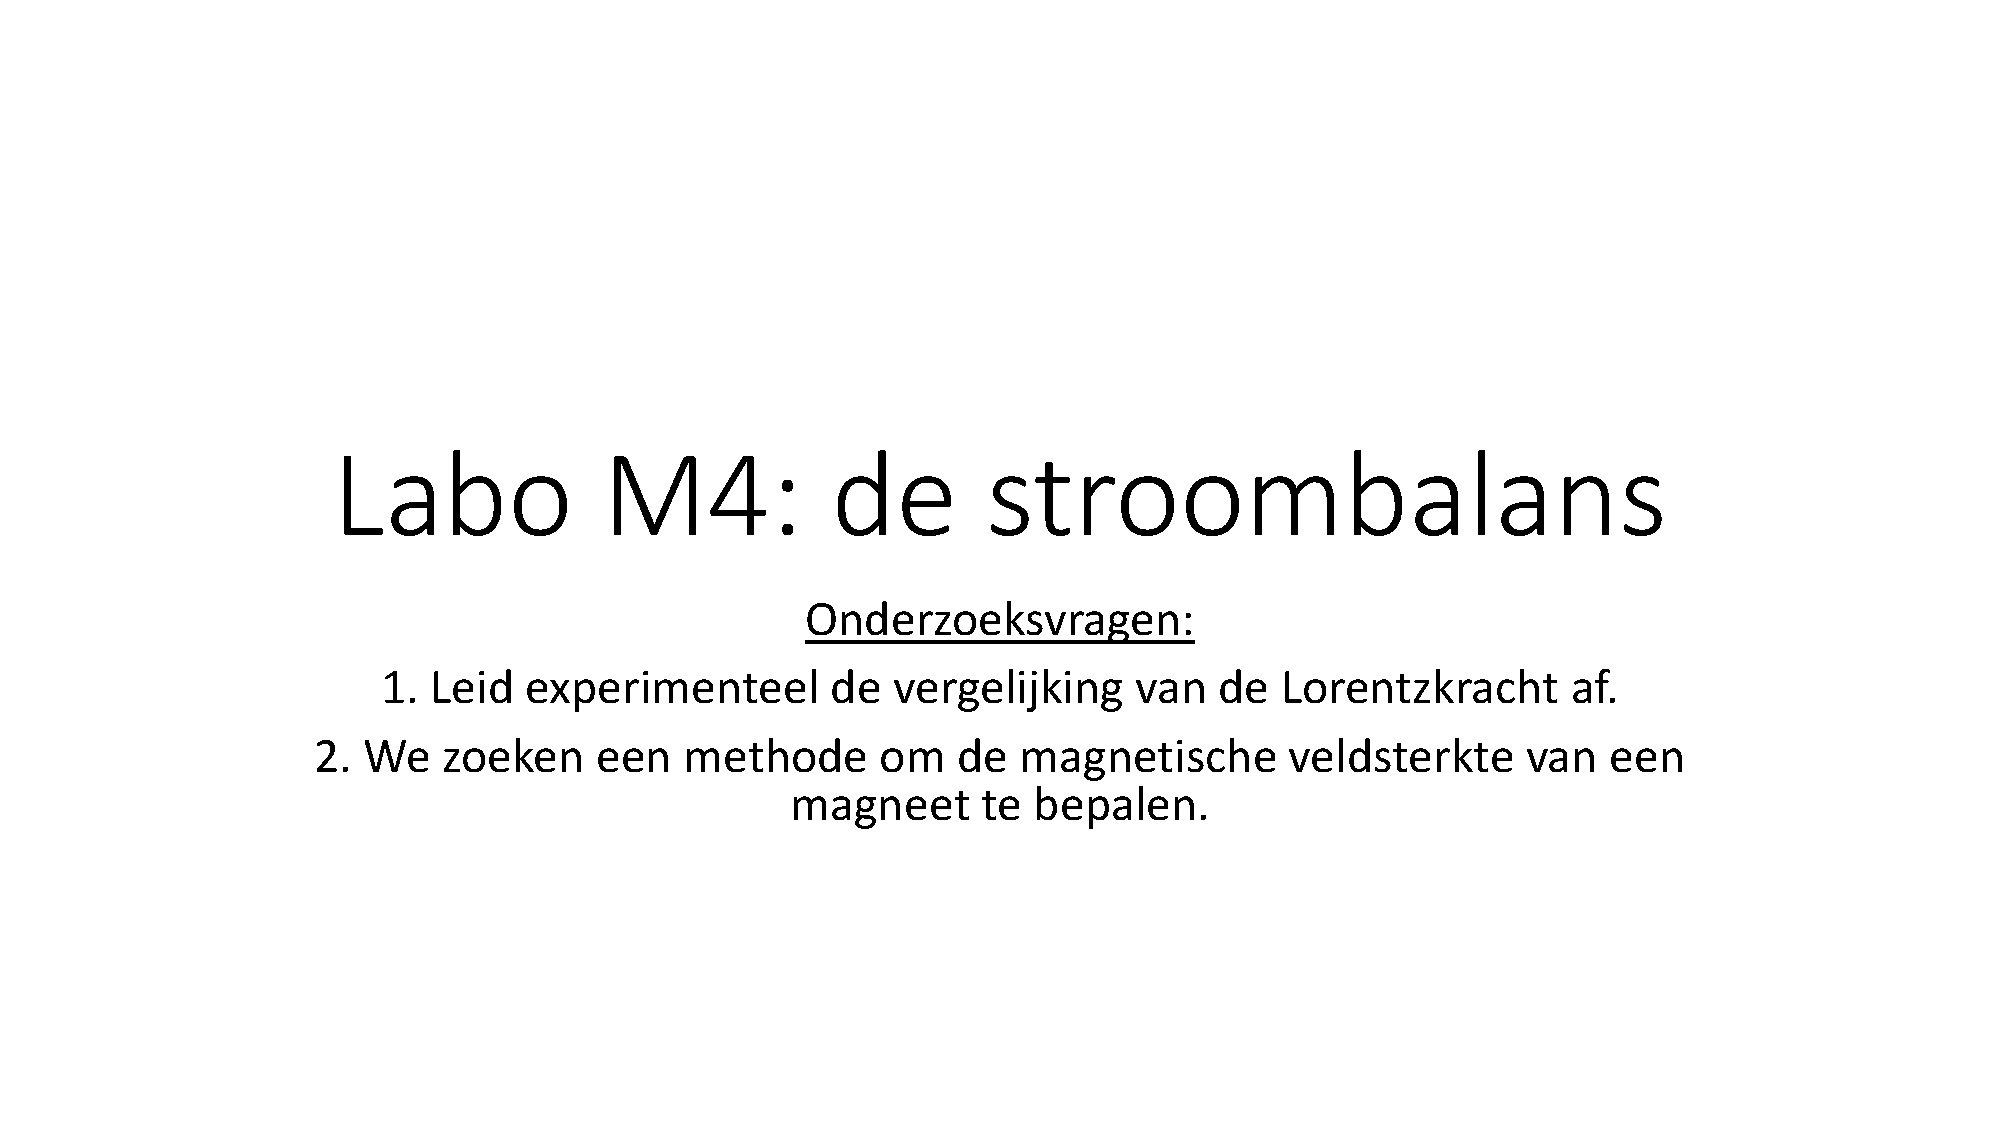
\includepdf[scale = 0.9, pages = -,pagecommand=\subsection*{Bijlage 4.2.1.1: slides introductie},nup=2x3, delta = 0.5cm 1cm]{LaboM4.pdf}
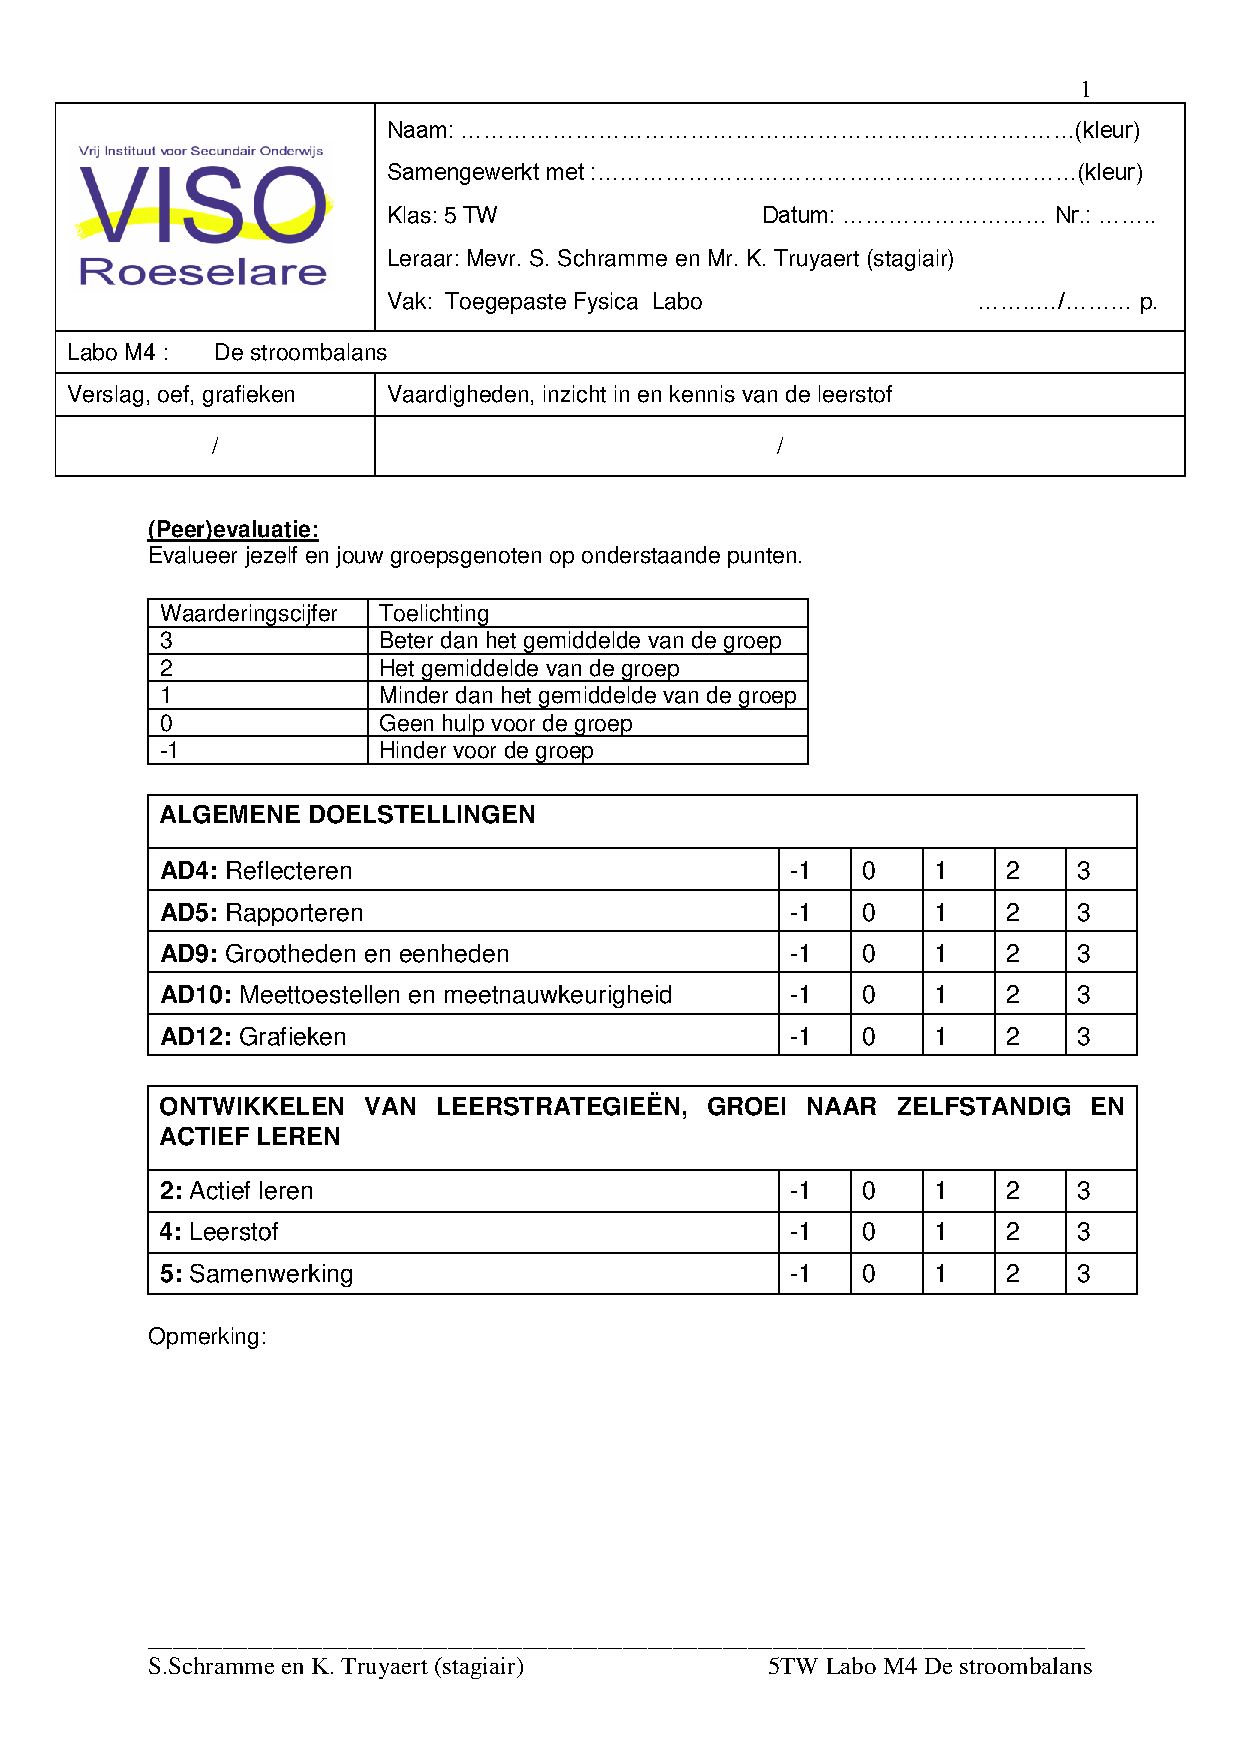
\includepdf[scale = 0.9, pages = 1,pagecommand=\subsection*{Bijlage 4.2.1.2: onderzoeksbundel over `De stroombalans'}]{M4Stroombalans1920.pdf}
\includepdf[scale = 0.9, pages = 2-,pagecommand=]{M4Stroombalans1920.pdf}

%
%\subsection*{Bijlage 1.2: bordschema theorie}
%\begin{center}
%	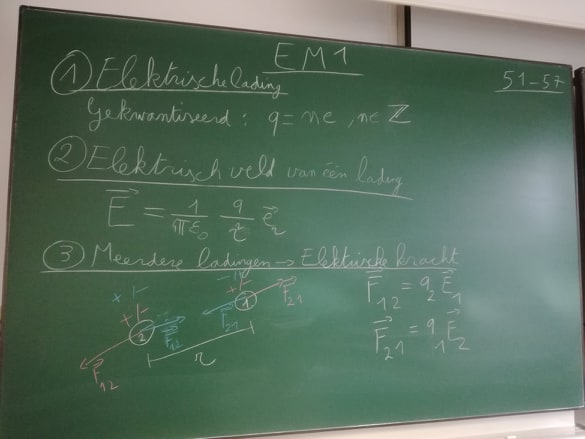
\includegraphics[width=0.9\textwidth]{Bord1a}
%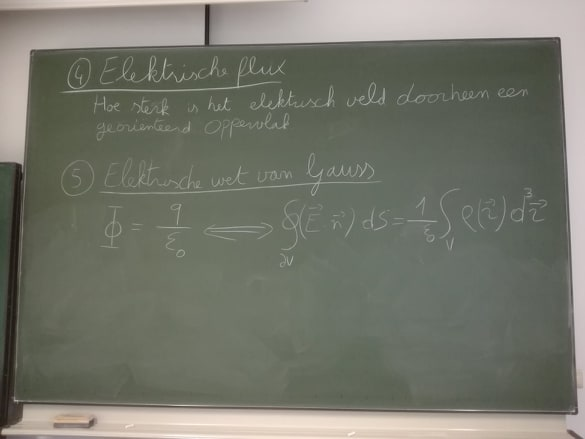
\includegraphics[width=0.9\textwidth]{Bord1b}
%\end{center}
%\newpage
%
%
%\includepdf[scale = 0.8,pages = 17,pagecommand=\subsection*{Bijlage 1.3: opgeloste oefeningen}]{Observaties_OpgelosteOef}
%\includepdf[scale = 0.8,pages =18-20,pagecommand=]{Observaties_OpgelosteOef}
%
%
%
%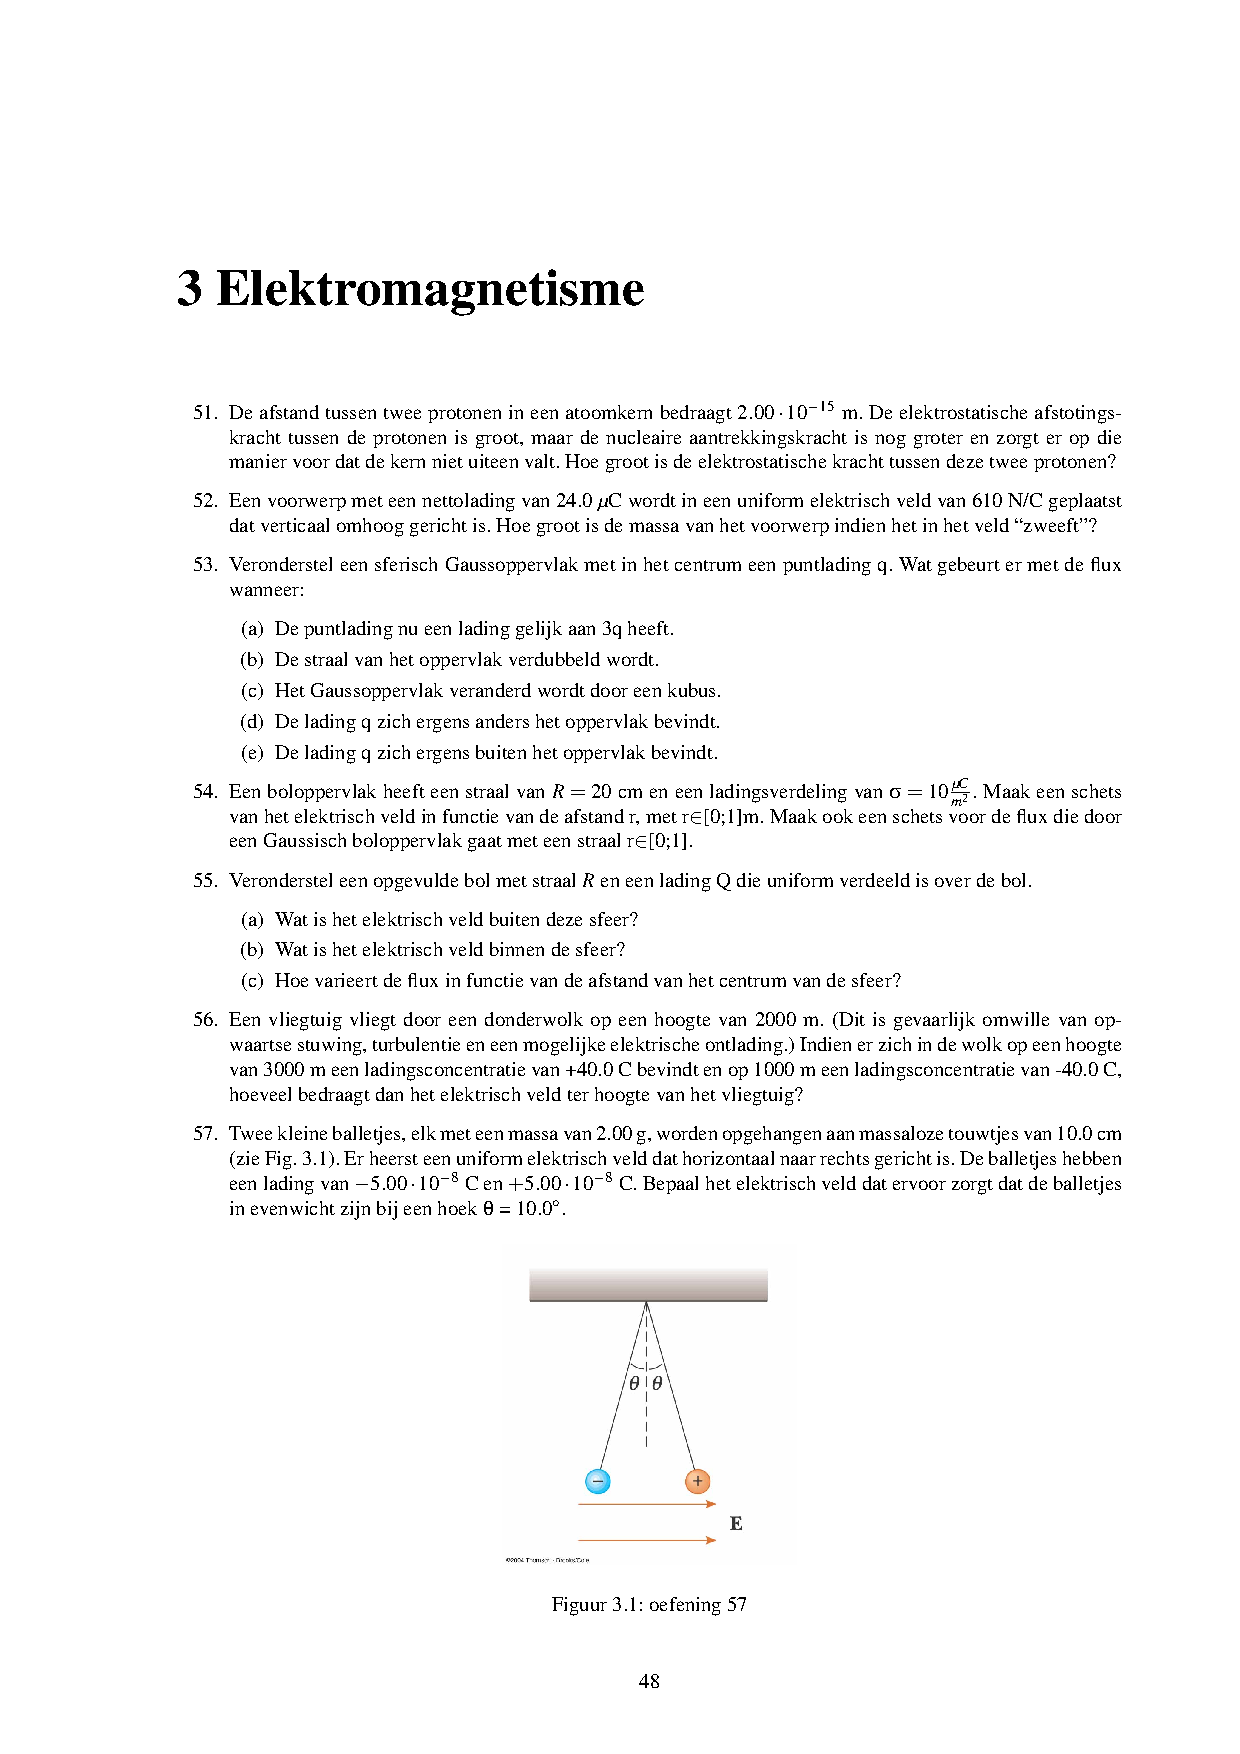
\includepdf[scale = 0.95,pages = 1,pagecommand=\subsection*{Bijlage 1.4: oefeningenbundel elektromagnetisme}]{OefeningenBundel}
%\includepdf[scale = 0.95,pages =2-,pagecommand=]{OefeningenBundel}
% !TeX root = Stageportfolio.tex



\begin{landscape}
	\subsubsection{Les 13}
	\begin{tabularx}{1.56\textwidth}{|p{0.35\textwidth}|X|}\hline
		\textbf{Administratieve gegevens}\newline\newline
		Kevin Truyaert\newline\newline
		technisch secundair onderwijs\newline
		3e graad, 1ste jaar, Techniek-Wetenschappen\newline
		VVKSO: \href{http://ond.vvkso-ict.com/leerplannen/doc/Toegepaste\%20fysica-2014-041.pdf}{http://ond.vvkso-ict.com/leerplannen /doc/Toegepaste\%20fysica-2014-041.pdf} \newline
		\underline{Lesonderwerp}:\newline Afwerken `Labo M4: De stroombalans' & \textbf{Doelstellingen}
		\begin{itemize}[itemsep=0.08\baselineskip]
			\item B24: De richting, de zin en de grootte van de Lorentzkracht op een rechte stroomvoerende geleider aangeven en hiermee de magnetische veldsterkte omschrijven. 
			\item AD4 Reflecteren: Over een waarnemingsopdracht/experiment/onderzoek en het resultaat reflecteren.
			\item AD5 Rapporteren: Over een waarnemingsopdracht/experiment/onderzoek en het resultaat rapporteren.
			\item AD10 Meettoestellen en meetnauwkeurigheid: De gepaste toestellen kiezen voor het meten van de behandelde grootheden en de meetresultaten correct aflezen en noteren.
			\item AD 12 Grafieken: Meetresultaten grafisch voorstellen in een diagram en deze interpreteren.
		\end{itemize}
		\underline{Lesdoelen}\newline
		\vspace{-0.75cm}
		\begin{enumerate}[itemsep=0.08\baselineskip]
			\item De leerlingen kunnen de Lorentzkracht toepassen op de specifieke situatie van de stroombalans.
			\item De leerlingen reflecteren over de resultaten.
			\item De leerlingen rapporteren over hun resultaten.
			\item De leerlingen werken samen bij het opbouwen van hun verslag.
			\item De leerlingen houden bij hun berekeningen rekening met de nauwkeurigheid.
			\item De leerlingen stellen de meetresultaten grafisch voor.
			\item De leerlingen berekenen de magnetische veldsterkte van de magneet.
			\item De leerlingen begrijpen conceptueel wat de magnetische flux is.
			\item De leerlingen kunnen de drie factoren die de magnetische flux bepalen.
		\end{enumerate} \\\hline
	\end{tabularx}


	\begin{tabularx}{1.56\textwidth}{|p{0.55\textwidth}|X|}
		\hline
		\multirow{2}{0.55\textwidth}{\textbf{Beginsituatie}\newline  
		Er zijn acht leerlingen binnen 5TW. Er heerst een algemene klassfeer. De leerlingen hebben al theorie gekregen  rond en oefeningen gemaakt op de magnetische krachtwerking. \newline\newline De leerlingen hebben de week voor de krokusvakantie aan dit labo mogen beginnen en hebben toen de metingen uitgevoerd. Ze zijn ook al begonnen met de verwerking van hun data. \newline\newline Hannah was vorige les afwezig. Ze zal deze les bij de groep waarbij ze ingedeeld was aansluiten.   \newline\newline Mijn vorige lessen (11-12) zijn algemeen gezien goed verlopen. Dit labo mag drie lessen in beslag nemen en dit zal zeker lukken. Het begin van volgende laboles zal ik echter wel wat anders aanpakken. Ook in het algemeen zal ik mij wat sterker moeten richten op de zwakkere leerlingen in de groep en de sterkere vooral zelfstandig laten bezig zijn, in plaats van voor wat extra verdiepende vragen aan die laatste groep te stellen.} & \textbf{Acties}\newline\newline  
		- \YellowHighlight{Ik herhaal de inhoud van het labo nog eens kort: waarover deden jullie onderzoek}{15cm}  \YellowHighlight{en wat waren de onderzoeksvragen?}{7cm} Door deze herhaling zorg ik ervoor dat de beginsituatie voor iedereen terug gelijk is en hoop ik dat de leerlingen terug kunnen inpikken na de krokusvakantie. \newline\newline
		- \GreenHighlight{Bij een labo is het de bedoeling om in groep een resultaat op de gestelde onderzoeks-}{15cm} \GreenHighlight{vragen te bekomen.}{3.6cm} Hier worden de leerlingen in drie groepen onder verdeeld. Hierdoor zal er een goede wisselwerking kunnen zijn tussen de leerlingen onderling en zijn er voldoende kritische blikken per groep om de vragen op te lossen. 
		\newline\newline\newline\newline\newline\newline\newline\newline
		
		\\ \cline{2-2}
		  & \textbf{Bronnen}\begin{itemize}
		  	\item Schramme, S. (2018) De stroombalans, labo magnetisme 4
		  	\item Frederiksen (2014), Current Balance 4565.00
		  \end{itemize}\\ \hline
	\end{tabularx}


\newpage
	
	\begin{tabularx}{1.56\textwidth}{|p{1.5cm}|p{9cm}|X|p{4cm}|}
		\hline
		\textbf{Nr. lesdoel } & \textbf{Inhoud (timing)}  & \textbf{Organisatie } & \textbf{Media } \\ \hline
		&\underline{Herhaling onderzoeksvragen} \underline{labo (5 minuten)}\newline
			De leerlingen krijgen hun bundel terug van mij en we overlopen de onderzoeksvragen van het labo nog even gezamenlijk. We gaan nog even dieper in op de effecten van de Lorentzkracht op de draad en de reactiekracht op de magneet.
		&  \underline{Onderwijsleergesprek}\newline 
			De leerlingen nemen plaats aan hun computer en krijgen hun bundel terug. Daarna overloop ik via vraagstelling aan de leerlingen nog eens de onderzoeksvragen van het labo. 
		&  Labobundel
		\\ \hline
	\end{tabularx}\vspace{5mm}

\begin{tabularx}{1.56\textwidth}{|p{1.5cm}|p{9cm}|X|p{4cm}|}
	\hline
	\textbf{Nr. lesdoel } & \textbf{Inhoud (timing)}  & \textbf{Organisatie } & \textbf{Media } \\ \hline
	1\newline\newline 2\newline\newline 3\newline\newline 4\newline\newline 5\newline\newline 6\newline\newline 7&\underline{Afwerken laboverslag magnetisme 4:} \underline{de stroombalans (35 minuten)}\newline
	De leerlingen zullen deze tijd nodig hebben om hun laboverslag af te werken. Ze zijn bezig met het afronden van onderdeel 6. Hierna bouwen ze een algemene conclusie op rond de Lorentzkracht, de stroomsterkte en de lengte van de geleider. Vanuit dit besluit, berekenen ze dan de veldsterkte van de magneet. Vijf van de acht leerlingen hebben op dit moment de fout gemaakt om niet met SI-eenheden te werken. Ik heb hier bewust nog niets over gezegd, zodat ze dit in hun besluit zullen ondervinden en bij zichzelf de vraag zullen moeten stellen wat er nu precies fout gelopen is. 
	&  \underline{Onderzoekspracticum}\newline 
	De leerlingen werken per groep verder aan hun individueel verslag. Ze  dienen individueel een verslag in, maar ze mogen nog met hun groepsleden samenwerken.
	
	
	&  Computers (computerlokaal)\newline\newline Labobundel
	\\ \hline
\end{tabularx}

\begin{tabularx}{1.56\textwidth}{|p{1.5cm}|p{9cm}|X|p{4cm}|}
	\hline
	\textbf{Nr. lesdoel } & \textbf{Inhoud (timing)}  & \textbf{Organisatie } & \textbf{Media } \\ \hline
	8\newline\newline 9&\underline{Introductie magnetisme hoofdstuk 5:  } \underline{ Elektromagnetische inductie:} \underline{de magnetische flux (10 minuten)}\newline
	Tijdens de resterende tijd wordt het concept van magnetische flux ingeleid. De figuur wordt op het bord getekend en de polen worden aangeduid. Enkel het concept van de magnetische flux wordt besproken, samen met de drie componenten waaruit die bestaat. Afhankelijk van de tijd worden er enkele eigenschappen besproken.
	&  \underline{Onderwijsleergesprek}\newline 
	Ik teken de situatie op het bord en stel gerichte vragen aan de leerlingen zodat zij de concretere eigenschappen van de situatie verwoorden (Hoe liggen de polen, hoe ligt de hoek $\alpha$ \ldots).
	
	
	&  Cursus hoofdstuk 5
	\\ \hline
\end{tabularx}


	
\end{landscape}


%\subsection*{Bijlage 5.1: slides introductie}

%
%\subsection*{Bijlage 1.2: bordschema theorie}
%\begin{center}
%	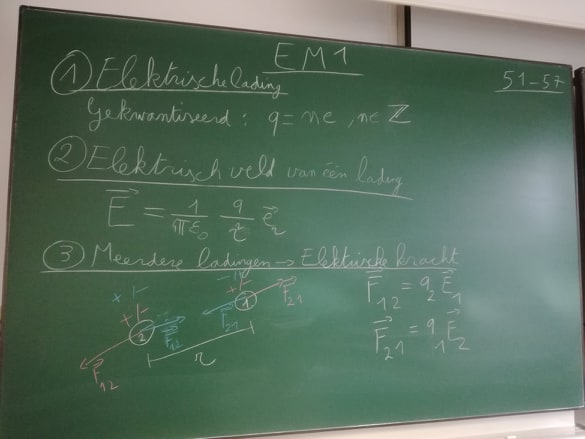
\includegraphics[width=0.9\textwidth]{Bord1a}
%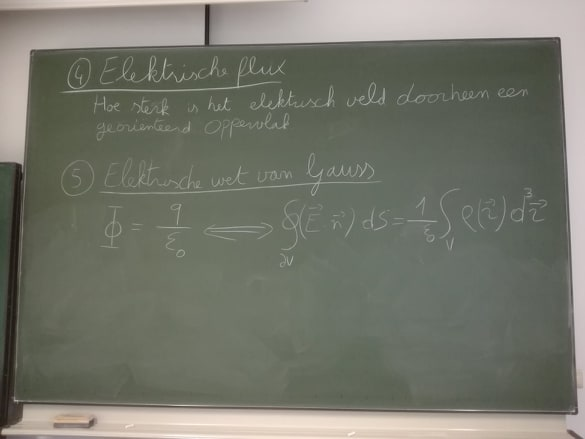
\includegraphics[width=0.9\textwidth]{Bord1b}
%\end{center}
%\newpage
%
%
%\includepdf[scale = 0.8,pages = 17,pagecommand=\subsection*{Bijlage 1.3: opgeloste oefeningen}]{Observaties_OpgelosteOef}
%\includepdf[scale = 0.8,pages =18-20,pagecommand=]{Observaties_OpgelosteOef}
%
%
%
%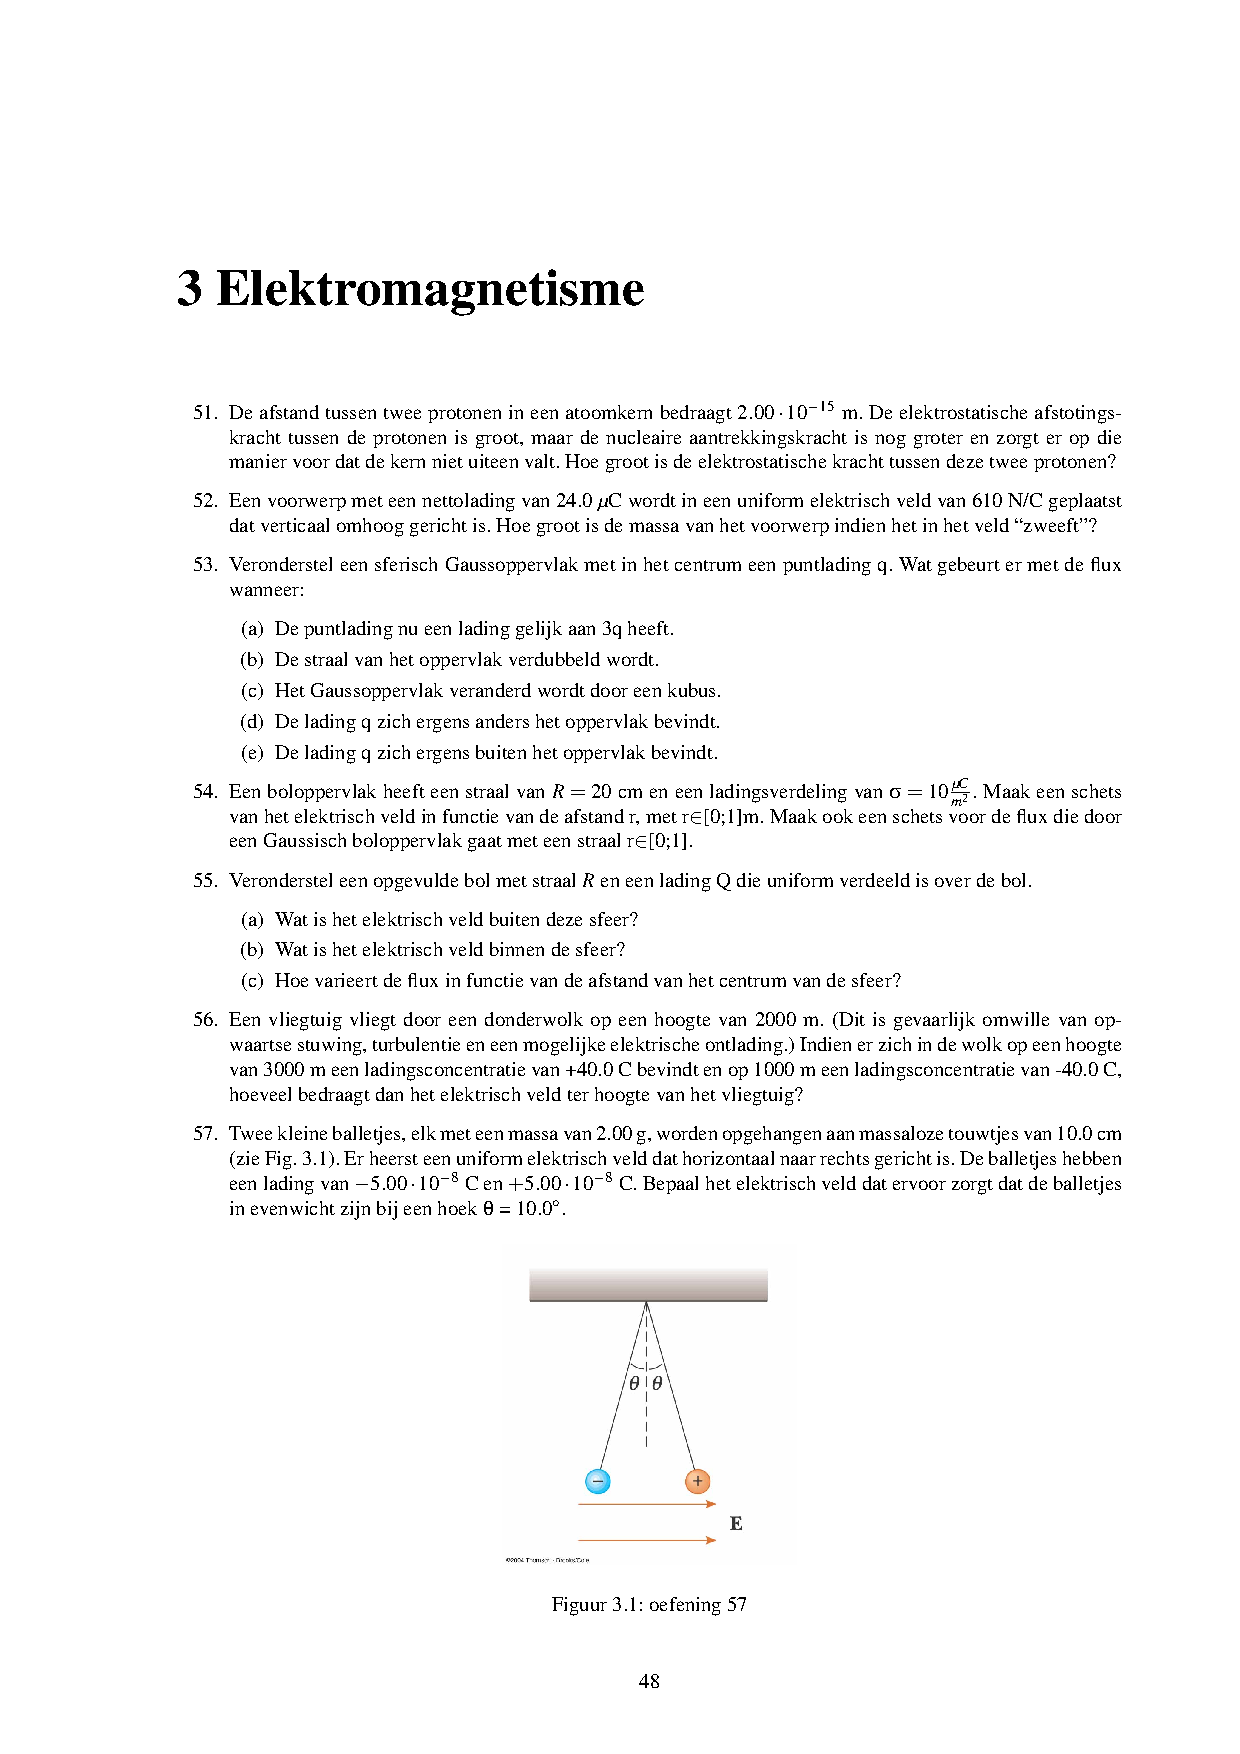
\includepdf[scale = 0.95,pages = 1,pagecommand=\subsection*{Bijlage 1.4: oefeningenbundel elektromagnetisme}]{OefeningenBundel}
%\includepdf[scale = 0.95,pages =2-,pagecommand=]{OefeningenBundel}
% !TeX root = Stageportfolio.tex



\begin{landscape}
	\subsubsection{Les 14-15}
	\begin{tabularx}{1.56\textwidth}{|p{0.35\textwidth}|X|}\hline
		\textbf{Administratieve gegevens}\newline\newline
		Kevin Truyaert\newline\newline
		technisch secundair onderwijs\newline
		3e graad, 1ste jaar, Techniek-Wetenschappen\newline
		VVKSO: \href{http://ond.vvkso-ict.com/leerplannen/doc/Toegepaste\%20fysica-2014-041.pdf}{http://ond.vvkso-ict.com/leerplannen /doc/Toegepaste\%20fysica-2014-041.pdf} \newline
		\underline{Lesonderwerp}:\newline Bespreking labo M4 \& Magnetische fluxverandering & \textbf{Doelstellingen}
		\begin{itemize}[itemsep=0.08\baselineskip]
			\item B27: Fluxverandering als oorzaak van inductiespanning toelichten
		\end{itemize}
		\underline{Lesdoelen}\newline
		\vspace{-0.75cm}
		\begin{enumerate}[itemsep=0.08\baselineskip]
			\item De leerlingen zien in hoe de lorentzkracht op de geleider een effect op een balans kan hebben.
			\item De leerlingen begrijpen conceptueel wat de magnetische flux is.ver
			\item De leerlingen kennen de drie factoren die de magnetische flux bepalen.
			\item De leerlingen kunnen de magnetische flux berekenen.
			\item De leerlingen begrijpen hoe een fluxverandering kan ontstaan.
			\item De leerlingen kunnen de fluxverandering berekenen.
			\item De leerlingen ervaren het ontstaan van een inductiespanning door middel van een fluxverandering via demo's.
			\item De leerlingen ervaren de analogie tussen elektriciteit en magnetisme bij het bespreken van inductieverschijnselen.
			\item De leerlingen kunnen de wet van Faraday zelf, via een demo, samenstellen.
		\end{enumerate} \\\hline
	\end{tabularx}\vfill \textcolor{white}{.} 


	\begin{tabularx}{1.56\textwidth}{|p{0.55\textwidth}|X|}
		\hline
		\multirow{2}{0.55\textwidth}{\textbf{Beginsituatie}\newline  
		Er zijn acht leerlingen binnen 5TW. Er heerst een algemene klassfeer. De leerlingen hebben al theorie gekregen  rond en oefeningen gemaakt op de magnetische krachtwerking. \newline\newline De leerlingen hebben de dag hiervoor hun labo ingediend. Vandaag worden de belangrijkste aspecten hiervan nog even overlopen. Daarnaast beginnen we aan een nieuw hoofdstuk in verband met de elektromagnetische inductie. \newline\newline NOG AANVULLEN MET LERAARKENMERKEN.} & \textbf{Acties}\newline\newline  
		- Magnetische flux is een concept dat niet voor te stellen valt. De gevolgen van deze flux kan je wel voorstellen en worden uitvoerig in hoofdstuk 6 besproken. Vooraleer je deze concepten echter kan beginnen te bespreken, moeten de leerlingen de basis van elektromagnetische inductie beheersen, waarvoor ze magnetische flux(verandering) moeten begrijpen. Toch verwacht ik dat de leerlingen hier vlot mee weg zullen zijn en wil ik veel in interactie treden met de leerlingen. \newline\newline
		- \GreenHighlight{Via demo's wil ik bepaalde onderwerpen starten.}{9cm}	Op die manier kan ik de interesse van de leerlingen wekken en kan ik fysische wetmatigheden hen effectief aantonen. Zo kunnen leerlingen op een klassikale manier zelfstandig dingen ontdekken.	
		\newline\newline\newline\newline\newline\newline\newline\newline
		
		\\ \cline{2-2}
		  & \textbf{Bronnen}\begin{itemize}
		  	\item Schramme, S. (2018) De stroombalans, labo magnetisme 4
		  	\item Frederiksen (2014), Current Balance 4565.00
		  	\item Giancoli, D. C. (2008). Physics for scientists and engineers. Pearson Education International.
		  \end{itemize}\\ \hline
	\end{tabularx}


\newpage
	
	\begin{tabularx}{1.56\textwidth}{|p{1.5cm}|p{9cm}|X|p{4cm}|}
		\hline
		\textbf{Nr. lesdoel } & \textbf{Inhoud (timing)}  & \textbf{Organisatie } & \textbf{Media } \\ \hline
		1	&\underline{Bespreking Labo M4:} \underline{de stroombalans (15 minuten)}\newline
			 We gaan nog even dieper in op de effecten van de Lorentzkracht op de draad en de reactiekracht op de magneet om duidelijk te verklaren waarom de balans verschillen kon opmeten.
		&  \underline{Onderwijsleergesprek}\newline 
			De leerlingen krijgen hun door mij verbeterde labobundel terug en we overlopen de onderzoeksvragen van het labo nog even gezamenlijk. Ik vraag aan de leerlingen wat zij als essentie van het labo ervaren hebben. Vanuit dat standpunt wordt het labo besproken. Hierna wordt er niet meer terug gekomen op dit labo. Een duidelijk begrip van de Lorentzkracht is nodig voor de laatste twee hoofdstukken van magnetisme.
		&  Labobundel\newline\newline Slides (zie bijlage)
		\\ \hline
	\end{tabularx}\vspace{5mm}



\begin{tabularx}{1.56\textwidth}{|p{1.5cm}|p{9cm}|X|p{4cm}|}
	\hline
	\textbf{Nr. lesdoel } & \textbf{Inhoud (timing)}  & \textbf{Organisatie } & \textbf{Media } \\ \hline
    2\newline\newline 3& \underline{Magnetische flux (5 minuten)}\newline
    Het concept van magnetische flux, wat vorige les ingeleid werd, wordt nu kort herhaald.
	&  \underline{Onderwijsleergesprek}\newline  
	Ik teken een situatie met een magnetische flux op bord en de leerlingen zeggen mij wat de belangrijke eigenschappen zijn in verband met magnetische flux.	Welke drie componenten zijn er belangrijk en hoe is de flux hiervan afhankelijk?
	&  Cursus hoofdstuk 5 p1-2\newline\newline Krijtbord
	\\ \hline
\end{tabularx}\vspace{5mm}


\begin{tabularx}{1.56\textwidth}{|p{1.5cm}|p{9cm}|X|p{4cm}|}
	\hline
	\textbf{Nr. lesdoel } & \textbf{Inhoud (timing)}  & \textbf{Organisatie } & \textbf{Media } \\ \hline
	4& \underline{Magnetische flux: Oefeningen (20 minuten)}\newline
	Aangezien de leerlingen net de eigenschappen van magnetische flux gezien hebben, maken we eerst wat oefeningen hierop. Zo kunnen de leerlingen een beter begrip hierover krijgen.
	&  \underline{Onderwijsleergesprek + oefeningen}\newline  Oefening 2 a en b maak ik klassikaal met de leerlingen samen. Hierna werken de leerlingen oefening 2 individueel af. Ik schrijf ook op bord dat de leerlingen verder kunnen gaan met oefeningen 4, 5 en 6. De eindoplossing van die oefeningen komen op bord, de werkwijze zal enkel van oefening 5 op bord komen indien nodig.
	&  Cursus hoofdstuk 5 p4-5\newline\newline Krijtbord
	\\ \hline
\end{tabularx}\vspace{5mm}


\begin{tabularx}{1.56\textwidth}{|p{1.5cm}|p{9cm}|X|p{4cm}|}
\hline
\textbf{Nr. lesdoel } & \textbf{Inhoud (timing)}  & \textbf{Organisatie } & \textbf{Media } \\ \hline
5& \underline{Magnetische fluxverandering: theorie (15 minuten)}\newline
Aangezien de leerlingen net de eigenschappen van magnetische flux gezien hebben, definieer ik nu de magnetische fluxverandering. De leerlingen komen te weten hoe die verandering tot stand kan komen.
&  \underline{Onderwijsleergesprek}\newline 
Ik teken een situatie met een magnetische flux op bord en de leerlingen zeggen mij wat de belangrijke eigenschappen zijn in verband met magnetische flux. Ik vraag de leerlingen hoe die fluxverandering kan ontstaan (net vanuit één van die drie eigenschappen). Zo bespreken we alle mogelijkheden van de opwekking van een fluxverandering.	
&  Cursus hoofdstuk 5\newline\newline Krijtbord
\\ \hline
\end{tabularx}\vspace{5mm}



\begin{tabularx}{1.56\textwidth}{|p{1.5cm}|p{9cm}|X|p{4cm}|}
	\hline
	\textbf{Nr. lesdoel } & \textbf{Inhoud (timing)}  & \textbf{Organisatie } & \textbf{Media } \\ \hline
	5\newline\newline 6& \underline{Magnetische fluxverandering:} \underline{Oefeningen (15 minuten)}\newline
	Aangezien de leerlingen net de eigenschappen van magnetische fluxverandering gezien hebben, maken we eerst wat oefeningen hierop, om een beter begrip van de fluxverandering te krijgen. Dat is essentieel om aan inductiespanning te kunnen beginnen.
	&  \underline{Onderwijsleergesprek + oefeningen}\newline  Oefening 7 maak ik klassikaal, met de leerlingen samen, via vraagstelling aan de leerlingen. Hierna werken de leerlingen individueel oefening 8 en 9. Ik schrijf enkel de tussenoplossingen en de eindoplossing op bord. Ondertussen plaats ik het materiaal voor de demo rond inductiespanning en -stroom op tafel.
	&  Cursus hoofdstuk 5 p5-6\newline\newline Krijtbord
	\\ \hline
\end{tabularx}\vspace{5mm}



\begin{tabularx}{1.56\textwidth}{|p{1.5cm}|p{9cm}|X|p{4cm}|}
	\hline
	\textbf{Nr. lesdoel } & \textbf{Inhoud (timing)}  & \textbf{Organisatie } & \textbf{Media } \\ \hline
	7\newline\newline 8& \underline{Inductiespanning en -stroom:} \underline{Inleiding (10 minuten)}\newline
	Er werd in vorige lessen (Hoofdstuk 2) door de leerlingen ondervonden dat een elektrische stroom een magnetisch veld veroorzaakt. Hier onderzoeken we of het omgekeerde ook waar is: induceert een magnetisch veld een elektrische stroom in een gesloten circuit? Dit zal een interactie tussen elektriciteit en magnetisme aan de leerlingen tonen.
	&  \underline{Demonstratie + Onderwijsleergesprek}\newline 
	De opstelling bestaat uit een spoel die aangesloten is aan een milliampèremeter, die zowel negatieve als positieve stromen kan meten. Daarna beweeg ik een magneet naar de spoel. Ik zeg niets en vraag aan de leerlingen wat zij beschrijven wat er gebeurt. Hier speel ik op in en treed ik in interactie met de leerlingen om van hen te horen wat zij ervaren wat er gebeurt.	Op basis hiervan interageer ik met de leerlingen om hen in hun bewoording te begeleiden. Hierna vullen we samen op basis van de demo pagina's 7 en 8 in.
	&  Cursus hoofdstuk 5 p7-8\newline\newline Krijtbord
	\\ \hline
\end{tabularx}\vspace{5mm}




\begin{tabularx}{1.56\textwidth}{|p{1.5cm}|p{9cm}|X|p{4cm}|}
	\hline
	\textbf{Nr. lesdoel } & \textbf{Inhoud (timing)}  & \textbf{Organisatie } & \textbf{Media } \\ \hline
	7\newline\newline 8\newline\newline 9& \underline{De wet van Faraday:} \underline{Verbanden (15 minuten)}\newline
	Er is nu aangetoond dat in een gesloten circuit er een inductie stroom is. We kunnen ditzelfde experiment doen, maar in plaats van een milliampèremeter aan de spoel aan te sluiten, sluit ik nu een voltagemeter aan. Hieruit is het mogelijk om de inductiespanning te meten door middel van een fluxverandering. Door verschillende wijzigingen aan de situatie toe te brengen, kunnen de leerlingen zelf bepaalde evenredigheden uit de demonstratie halen. Samen met de leerlingen leid ik de wet van Faraday af.
	&  \underline{Demonstratie + Onderwijsleergesprek}\newline 
	De opstelling bestaat uit een spoel die aangesloten is aan een voltagemeter, die zowel negatieve als positieve spanningen kan meten. Daarna beweeg ik een magneet naar de spoel. Ik zeg niets en vraag aan de leerlingen wat zij beschrijven wat er gebeurt. Hier speel ik op in en treed ik in interactie met de leerlingen om van hen te horen wat zij ervaren wat er gebeurt.	Deze resultaten zullen ze snel begrijpen, gezien we net de situatie van de inductiestroom gezien hebben. Nu verander ik de windingen van de spoel, de flux (door middel van de magneet) en de tijdspanne waarin ik de magneet dichter breng. Deze relaties leiden uiteindelijk tot de wet van Faraday. Hierna vullen we samen op basis van de demo pagina's 9 en 10 in.
	&  Cursus hoofdstuk 5 p9-10\newline\newline Krijtbord
	\\ \hline
\end{tabularx}\vspace{5mm}


\begin{tabularx}{1.56\textwidth}{|p{1.5cm}|p{9cm}|X|p{4cm}|}
	\hline
	\textbf{Nr. lesdoel } & \textbf{Inhoud (timing)}  & \textbf{Organisatie } & \textbf{Media } \\ \hline
	& \underline{Slot (5 minuten)}\newline
	Ik herhaal nog even kort samen met de leerlingen de wet van Faraday. We bespreken samen wat deze voorstelt, een inductiespanning, en waarop deze steunt, een fluxverandering. Op deze manier probeer ik de leerlingen te evalueren.
	&  \underline{Vertellen}\newline 
	Bespreken van de wet van Faraday en fluxverandering
	&  
	\\ \hline
\end{tabularx}




	
\end{landscape}


%\subsection*{Bijlage 5.1: slides introductie}

%
%\subsection*{Bijlage 1.2: bordschema theorie}
%\begin{center}
%	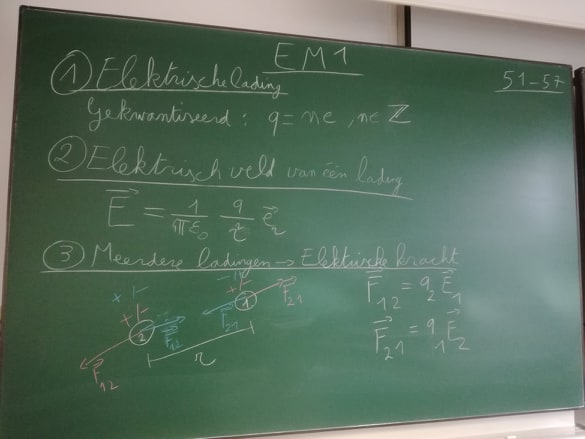
\includegraphics[width=0.9\textwidth]{Bord1a}
%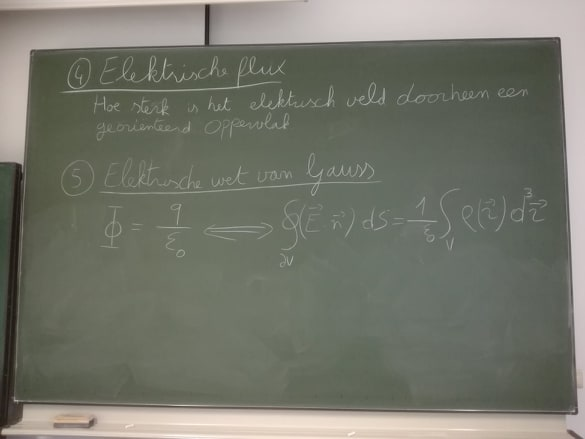
\includegraphics[width=0.9\textwidth]{Bord1b}
%\end{center}
%\newpage
%
%
%\includepdf[scale = 0.8,pages = 17,pagecommand=\subsection*{Bijlage 1.3: opgeloste oefeningen}]{Observaties_OpgelosteOef}
%\includepdf[scale = 0.8,pages =18-20,pagecommand=]{Observaties_OpgelosteOef}
%
%
%
%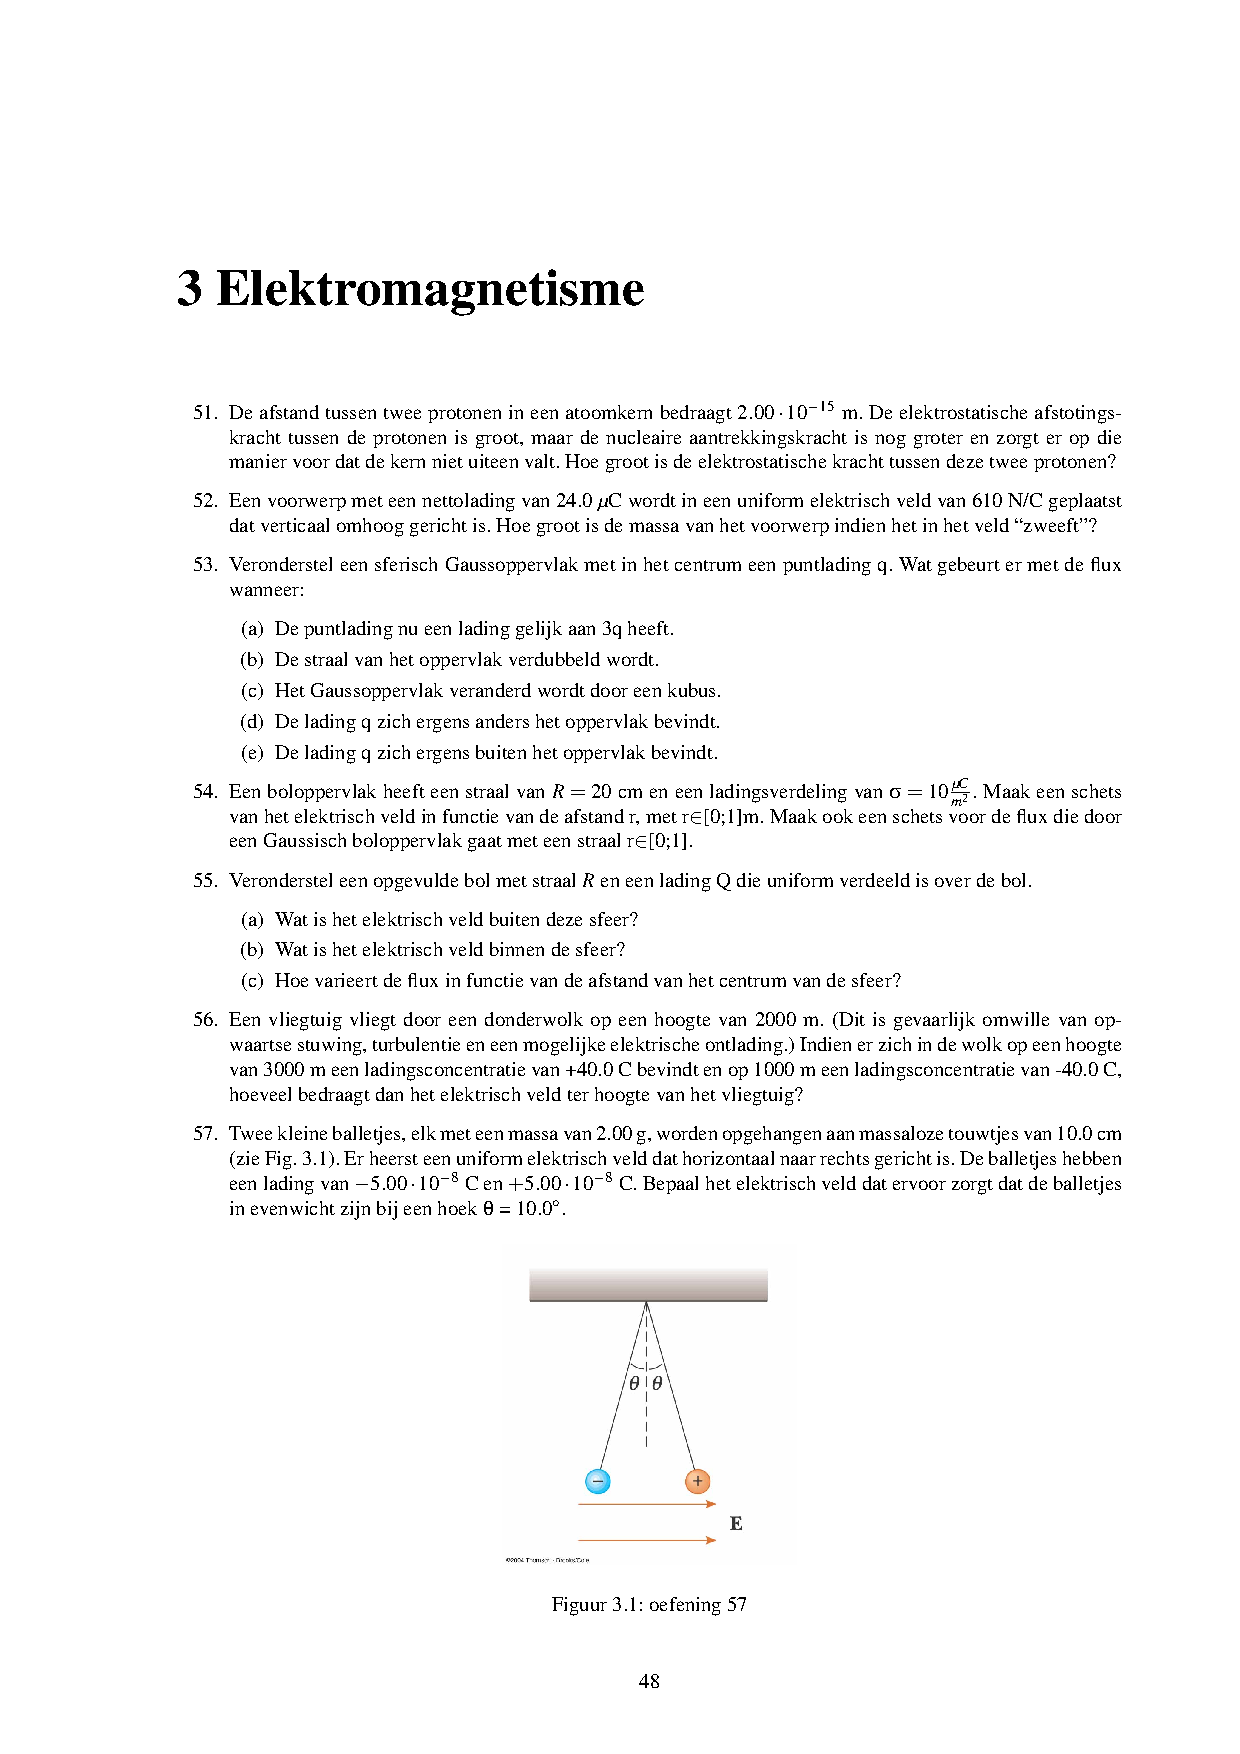
\includepdf[scale = 0.95,pages = 1,pagecommand=\subsection*{Bijlage 1.4: oefeningenbundel elektromagnetisme}]{OefeningenBundel}
%\includepdf[scale = 0.95,pages =2-,pagecommand=]{OefeningenBundel}
% !TeX root = Stageportfolio.tex



\begin{landscape}
	\subsubsection{Les 18}
	\begin{tabularx}{1.56\textwidth}{|p{0.35\textwidth}|X|}\hline
		\textbf{Administratieve gegevens}\newline\newline
		Kevin Truyaert\newline\newline
		technisch secundair onderwijs\newline
		3e graad, 1ste jaar, Techniek-Wetenschappen\newline
		VVKSO: \href{http://ond.vvkso-ict.com/leerplannen/doc/Toegepaste\%20fysica-2014-041.pdf}{http://ond.vvkso-ict.com/leerplannen /doc/Toegepaste\%20fysica-2014-041.pdf} \newline
		\underline{Lesonderwerp}:\newline  De wet van Lenz invullen \& algemene inductiewet: Faraday-Lenz + oefeningen & \textbf{Doelstellingen}
		\begin{itemize}[itemsep=0.08\baselineskip]
			\item B27: Fluxverandering als oorzaak van inductiespanning toelichten
			\item B28: Met behulp van de wet van Lenz de zin van de inductiespanning vinden
			\item B29: De algemene inductiewet hanteren.
		\end{itemize}
		\underline{Lesdoelen}\newline
		\vspace{-0.75cm}
		\begin{enumerate}[itemsep=0.08\baselineskip]
			\item De leerlingen kunnen de zin van de inductiestroom bepalen.
			\item De leerlingen kunnen de wet van Lenz verwoorden.
			\item De leerlingen kunnen de samenhang tussen de wet van Faraday en de wet van Lenz uitleggen.
			\item De leerlingen kunnen de wet van Faraday-Lenz reproduceren.
			\item De leerlingen kunnen de wet van Faraday-Lenz op een rechte, bewegende geleider toepassen.
			\item De leerlingen kunnen de algemene inductiewet tijdens oefeningen hanteren.
		\end{enumerate} \\\hline
	\end{tabularx}\vfill \textcolor{white}{.} 


	\begin{tabularx}{1.56\textwidth}{|p{0.55\textwidth}|X|}
		\hline
		\multirow{2}{0.55\textwidth}{\textbf{Beginsituatie}\newline  
		Er zijn acht leerlingen binnen 5TW. Er heerst een algemene klassfeer. De leerlingen hebben al theorie gekregen  rond en oefeningen gemaakt op de magnetische krachtwerking. \newline\newline De leerlingen hebben vorige week de wet van Faraday en Lenz gezien. Hiermee kunnen ze de grootte en de zin van de inductiespanning bepalen. Ook met de begrippen flux en fluxverandering zijn ze gekend. \newline\newline Vorige les heb ik uitgebreide feedback van zowel de vakmentor als de stage begeleider verkregen. Deze wil ik in deze en komende lessen proberen te integreren. De grootste bemerking waar ik rekening mee wil houden is dat ik nog meer van de leerlingen zelf mag laten komen, door hen bijvoorbeeld aan bord oefeningen te laten bespreken.} & \textbf{Acties}\newline\newline %Vandaag worden de belangrijkste aspecten hiervan nog even overlopen. Daarnaast zijn we gisteren ook begonnen aan een nieuw stuk theorie rond elektromagnetische inductie. Hiervan hebben we de basis rond magnetische flux al besproken. Dit wordt nog even terug aangehaald.
		- \GreenHighlight{Via demo's wil ik bepaalde onderwerpen starten.}{9cm}	Op die manier kan ik de interesse van de leerlingen wekken en kan ik fysische wetmatigheden hen effectief aantonen. Zo kunnen leerlingen op een klassikale manier zelfstandig dingen ontdekken.	 \newline\newline 
		- Ik wil oefeningen op zo'n wijze brengen dat ze steeds dezelfde structuur hebben. Die structuur bouw ik eerst samen met de leerlingen op, om ze daarna zelfstandig aan de slag te laten gaan met oefeningen die steeds wat complexer worden. \PinkHighlight{Tijdens het zelfstandig maken van de oefeningen probeer ik toch zeker}{13cm} \PinkHighlight{de zwakkere leerlingen in de gaten te houden en hen individueler te coachen bij het}{15cm} \PinkHighlight{maken van oefeningen.}{4.5cm}
		Bij het maken van die oefeningen zal ik de leerlingen wat meer zelf laten doen.
		\newline\newline\newline\newline
		
		\\ \cline{2-2}
		  & \textbf{Bronnen}\begin{itemize}
		  	\item Schramme, S. (2018-2019) Cursus hoofdstuk 5: elektromagnetische inductie
		  	\item Giancoli, D. C. (2008). Physics for scientists and engineers. Pearson Education International.
		  \end{itemize}\\ \hline
	\end{tabularx}


\newpage
	


\begin{tabularx}{1.56\textwidth}{|p{1.5cm}|p{8cm}|X|p{4cm}|}
	\hline
	\textbf{Nr. lesdoel } & \textbf{Inhoud (timing)}  & \textbf{Organisatie } & \textbf{Media } \\ \hline
	1\newline\newline 2&\underline{De wet van Lenz (10 minuten)}\newline
	Invullen pagina 11\& 12 gebeurde thuis nadat de demo uitvoerig besproken geweest is tijdens vorige les: nu overlopen + eventuele vragen van de leerlingen bespreken
	&  \underline{Onderwijsleergesprek}\newline 
	Projectie: figuur pagina 11 = weergave demo\newline
	Bespreken pagina's 11 en 12\newline
	Aandachtspunt: nogmaals hameren dat fluxverandering de oorzaak is door:
	\begin{itemize}
		\item vraag hen wat essentieel is voor inductiespanning
		\item Hoe ontstaat fluxverandering?
	\end{itemize}
	&   Cursus hoofdstuk 5 p11-12\newline\newline Krijtbord + projectie \newline\newline Elekromagneet, weekijzeren kern, hangende ring
	\\ \hline
\end{tabularx}\vspace{5mm}

	
\begin{tabularx}{1.56\textwidth}{|p{1.5cm}|p{8cm}|X|p{4cm}|}
	\hline
	\textbf{Nr. lesdoel } & \textbf{Inhoud (timing)}  & \textbf{Organisatie } & \textbf{Media } \\ \hline
	2\newline\newline 3\newline\newline &\underline{De algemene inductiewet:} \underline{Faraday-Lenz (5 minuten)}\newline
	De wet van Faraday-Lenz = combinatie van de wet van Faraday en de wet van Lenz.
	&  \underline{Onderwijsleergesprek}\newline 
	Bespreken van de wet:\newline
	$U_i(t) = -N\cdot\frac{\Delta \Phi}{\Delta t}$ Welke termen komen uit Faraday, welke uit Lenz? Wat vertelt dit juist opnieuw?
	&   Cursus hoofdstuk 5 p13\newline\newline Krijtbord 
	\\ \hline
\end{tabularx}\vspace{5mm}


\begin{tabularx}{1.56\textwidth}{|p{1.5cm}|p{8cm}|X|p{4cm}|}
	\hline
	\textbf{Nr. lesdoel } & \textbf{Inhoud (timing)}  & \textbf{Organisatie } & \textbf{Media } \\ \hline
	4\newline\newline 5&\underline{Faraday-Lenz op een rechte, bewegende} \underline{geleider (10 minuten)}\newline
	Toepassen van Faraday-Lenz op een bewegende geleider.
	&  \underline{Onderwijsleergesprek}\newline
	Situatie van bewegende geleider schetsen\newline	
	Lln zelf afleidingen proberen te maken, inpikken na enkele minuten\newline 
	Afleiden vergelijking: $|\Delta\Phi|=B(A_2-A_1)\cos(\alpha)=Bl\Delta x\cos(\alpha)$\newline
	Afleiden vergelijking: $\left|\frac{\Delta\Phi}{\Delta t}\right|=\frac{B(A_2-A_1)\cos(\alpha)}{\Delta t} = Bl\frac{\Delta x}{\Delta t}\cos(\alpha)= Blv\cos(\alpha)$
	&   Cursus hoofdstuk 5 p13\newline\newline Krijtbord 
	\\ \hline
\end{tabularx}\vspace{5mm}



\begin{tabularx}{1.56\textwidth}{|p{1.5cm}|p{6.5cm}|X|p{4cm}|}
	\hline
	\textbf{Nr. lesdoel } & \textbf{Inhoud (timing)}  & \textbf{Organisatie } & \textbf{Media } \\ \hline
    1\newline\newline 4 \newline\newline 7& \underline{Faraday-Lenz:} \underline{oefeningen (14 minuten)}\newline
    De leerlingen maken oefeningen op Faraday-Lenz.	
	&  \underline{Oefeningen}\newline
	\underline{Klassikaal:} Oefening 1 \underline{lln zelf aan bord komen uitleggen} \newline
	\underline{Check-in duo:} Oefening 2 (hoek), 3 (oppervlakte)\newline
	Zeggen dat oefening 4 over fluxverandering via B gaat.
	\underline{Grondigere reflectie na oefening 2,} 
	&  Cursus hoofdstuk 5 p14-15\newline\newline Krijtbord \newline\newline Projectie oef 1
	\\ \hline
\end{tabularx}\vspace{5mm}


\begin{tabularx}{1.56\textwidth}{|p{1.5cm}|p{6.5cm}|X|p{4cm}|}
	\hline
	\textbf{Nr. lesdoel } & \textbf{Inhoud (timing)}  & \textbf{Organisatie } & \textbf{Media } \\ \hline
	7	&\underline{Oefeningen: de algemene} \underline{inductiewet (10 minuten)}\newline
	Oefeningen op Faraday-Lenz: Oefeningen 6, 7, 9 en 11 (8 als reserve) 
	&  \underline{Zelfstandig oefeningen maken} \underline{Bespreking via correctiesleutel}\newline 
	- Leerlingen werken per twee\newline
	- Oefeningen maken terwijl ik observeer\newline
	- Leerlingen nemen zelf een oplossingssleutel (Met acht leerlingen kan ik in de gaten houden dat niemand zomaar een oplossingssleutel neemt)\newline\newline
	Morgen vervolg
	&   Cursus hoofdstuk 5 p15-16\newline\newline Krijtbord voor eventuele extra uitleg \newline\newline Correctiesleutels (4 per oefening)
	\\ \hline
\end{tabularx}\vspace{5mm}




\begin{tabularx}{1.56\textwidth}{|p{1.5cm}|p{6.5cm}|X|p{4cm}|}
	\hline
	\textbf{Nr. lesdoel } & \textbf{Inhoud (timing)}  & \textbf{Organisatie } & \textbf{Media } \\ \hline
	& \underline{Slot (1 minuut)}\newline
	Algemene inductiewet herhalen	
	&  \underline{Vertellen}\newline 
	&  Cursus hoofdstuk 5 \newline\newline Krijtbord
	\\ \hline
\end{tabularx}

	
\end{landscape}


%\subsection*{Bijlage 5.1: slides introductie}

%
%\subsection*{Bijlage 1.2: bordschema theorie}
%\begin{center}
%	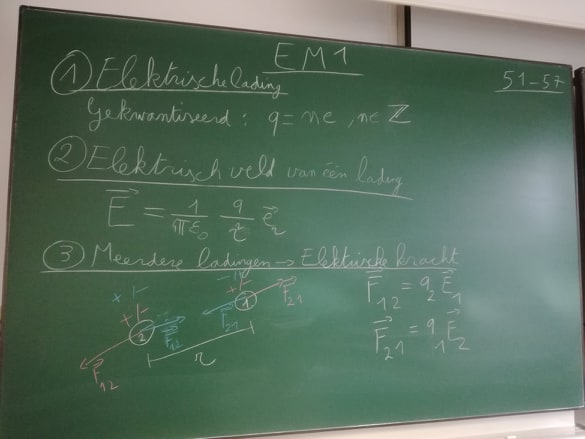
\includegraphics[width=0.9\textwidth]{Bord1a}
%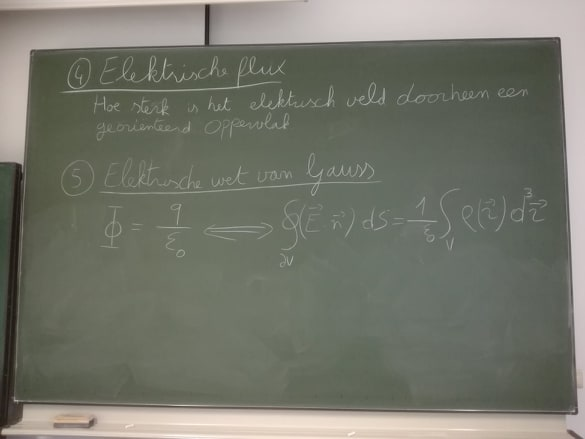
\includegraphics[width=0.9\textwidth]{Bord1b}
%\end{center}
%\newpage
%
%
%\includepdf[scale = 0.8,pages = 17,pagecommand=\subsection*{Bijlage 1.3: opgeloste oefeningen}]{Observaties_OpgelosteOef}
%\includepdf[scale = 0.8,pages =18-20,pagecommand=]{Observaties_OpgelosteOef}
%
%
%
%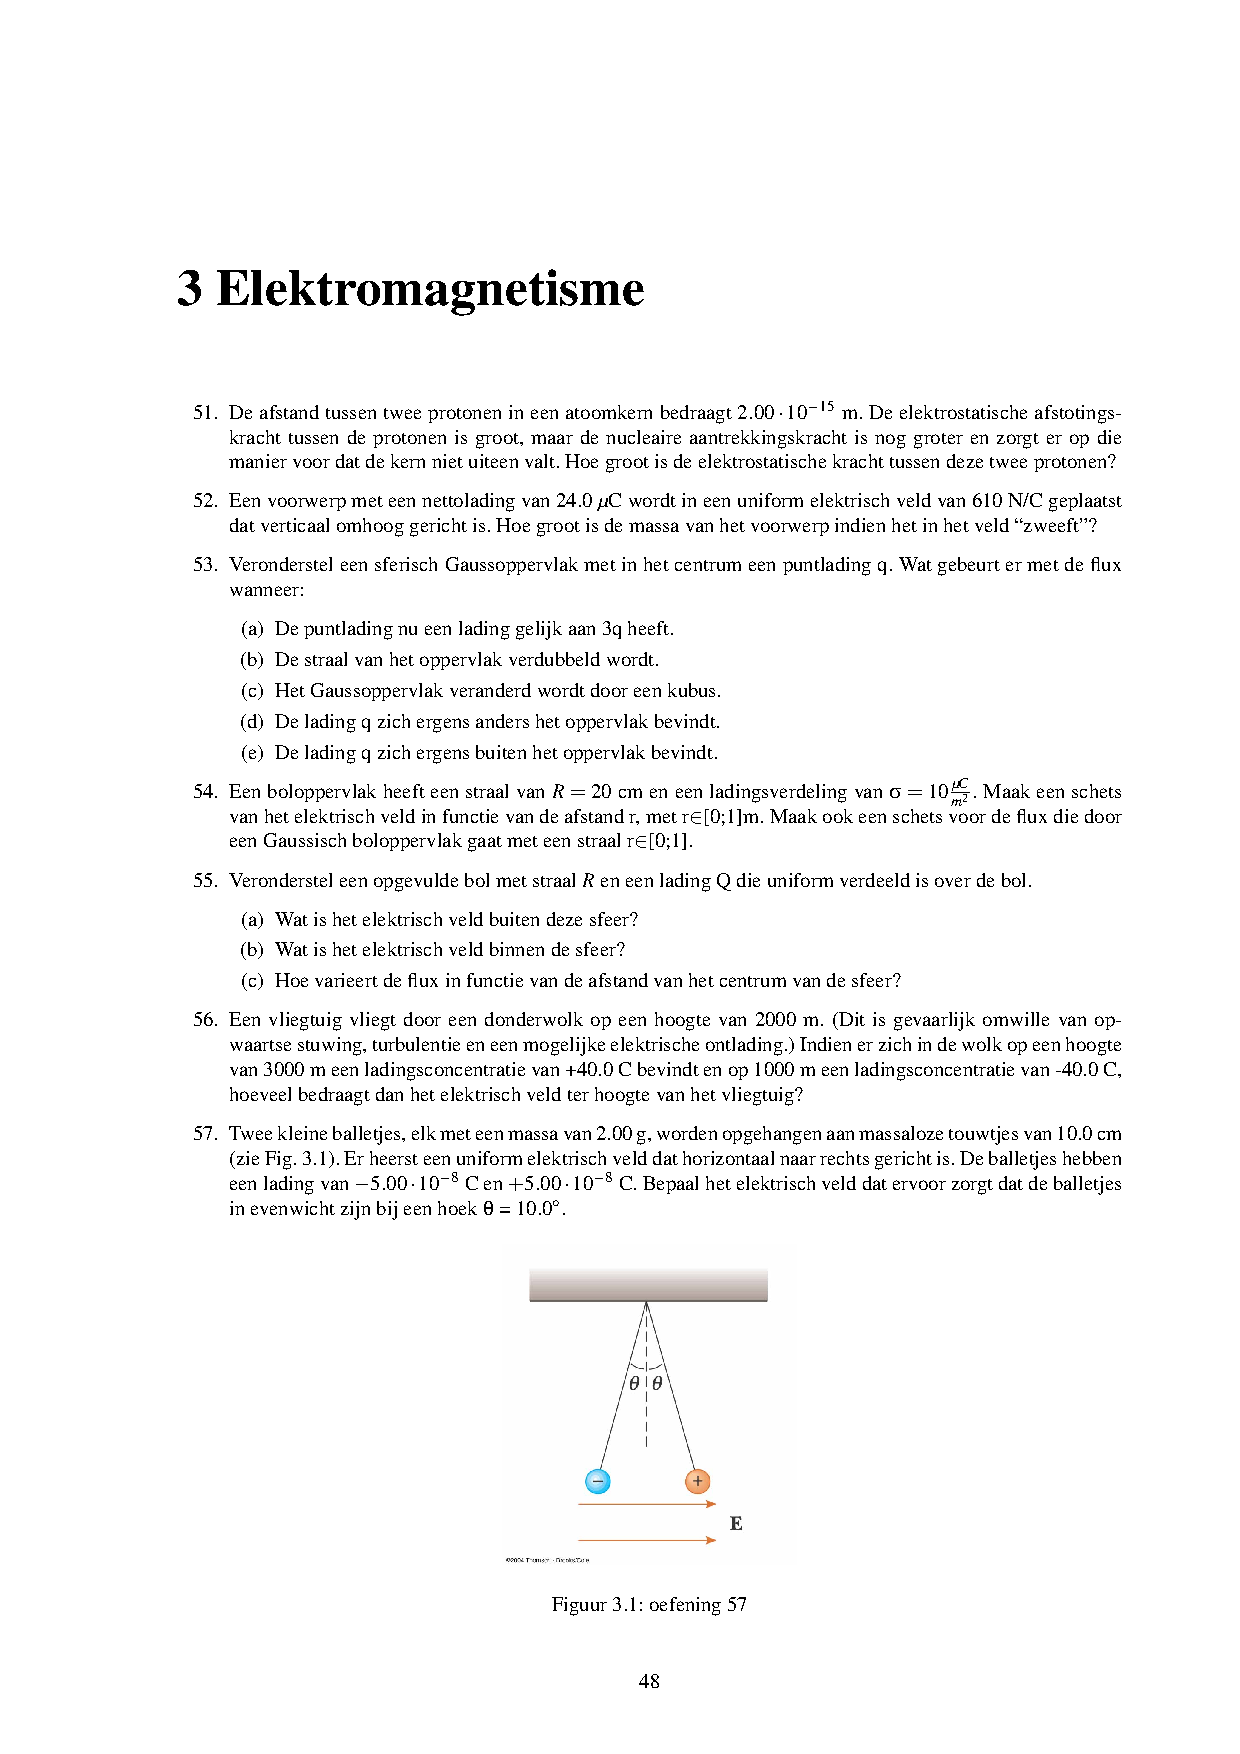
\includepdf[scale = 0.95,pages = 1,pagecommand=\subsection*{Bijlage 1.4: oefeningenbundel elektromagnetisme}]{OefeningenBundel}
%\includepdf[scale = 0.95,pages =2-,pagecommand=]{OefeningenBundel}	
% !TeX root = Stageportfolio.tex



\begin{landscape}
	\subsubsection{Les 19-20}
	\begin{tabularx}{1.56\textwidth}{|p{0.35\textwidth}|X|}\hline
		\textbf{Administratieve gegevens}\newline\newline
		Kevin Truyaert\newline\newline
		technisch secundair onderwijs\newline
		3e graad, 1ste jaar, Techniek-Wetenschappen\newline
		VVKSO: \href{http://ond.vvkso-ict.com/leerplannen/doc/Toegepaste\%20fysica-2014-041.pdf}{http://ond.vvkso-ict.com/leerplannen /doc/Toegepaste\%20fysica-2014-041.pdf} \newline
		\underline{Lesonderwerp}:\newline Bespreking labo M4\& Oefeningen op de algemene inductiewet \& Toepassingen op inductie & \textbf{Doelstellingen}
		\begin{itemize}[itemsep=0.08\baselineskip]
			\item B28: Met behulp van de wet van Lenz de zin van de inductiespanning vinden.
			\item B29: De algemene inductiewet hanteren.
			\item B30: Het werkingsprincipe van een generator weergeven.
			\item B31: De transformatorhouding bij de spanningen en de stromen van een ideale transformator toepassen en zijn functie bij het transport van elektrische energie toelichten.
		\end{itemize}
		\underline{Lesdoelen}\newline
		\vspace{-0.75cm}
		\begin{enumerate}[itemsep=0.08\baselineskip]
			\item De leerlingen reflecteren over het gemaakte labo.
			\item De leerlingen kunnen de wet van Faraday-Lenz op een rechte, bewegende geleider toepassen.
			\item De leerlingen kunnen de algemene inductiewet tijdens oefeningen hanteren.
			\item De leerlingen kunnen de werking van een wisselspanningsgenerator uitleggen.
		\end{enumerate} \\\hline
	\end{tabularx}\vfill \textcolor{white}{.} 


	\begin{tabularx}{1.56\textwidth}{|p{0.55\textwidth}|X|}
		\hline
		\multirow{2}{0.55\textwidth}{\textbf{Beginsituatie}\newline  
		Er zijn acht leerlingen binnen 5TW. Er heerst een algemene klassfeer. De leerlingen hebben al theorie gekregen rond en basisoefeningen gemaakt op elektromagnetische inductie. Ze zijn hier al vlot mee weg.  \newline\newline 
		De leerlingen hebben gisteren oefeningen over de wet van Faraday en Lenz gezien. Van hieruit vertrekken we nu om een toepassing te bespreken. \newline\newline Vorige les verliep iets minder goed op vlak van aanspreken van leerlingen. Ik vond dat ik terugviel op mijn veiligheid en zelf veel vertelde. Deze les wil ik het anders aanpakken en de leerlingen echt aan het woord laten.
		} & \textbf{Acties}\newline\newline  
		- Bij het aanbrengen van de toepassing, de wisselspanningsgenerator, wil ik al eens \YellowHighlight{afvoelen wat de leerlingen hiervan weten}{7.5cm}. Eens dit onderwerp geïntroduceerd is, zal ik vragen of de leerlingen hier voorbeelden van kennen, zoals een windmolen. Op die manier wil ik bereiken dat ze het onderwerp interessant vinden, doordat ze het met fysieke zaken kunnen linken. \newline\newline 
		- Bij het afleiden van de werking van de wisselspanningsgenerator wil ik er echt voor zorgen dat de leerlingen de afleiding maken. Ik wil ook \PinkHighlight{iedereen aan bod laten komen}{5.5cm} om het topic te bespreken, iets wat zeker mogelijk is gezien de vele stappen in het proces, om te toetsen of ze het Faraday-Lenz beheersen.\newline\newline
		- Ik wil de leerlingen op zelfstandige basis oefeningen laten maken. Ik loop ter controle rond, maar het zijn de leerlingen zelf die hun oefeningen controleren met behulp van een \GreenHighlight{oplossingsfiche}{2.8cm}. \newline\newline
		\\ \cline{2-2}
		  & \textbf{Bronnen}\begin{itemize}
		  	\item Schramme, S. (2018-2019) Cursus hoofdstuk 5: elektromagnetische inductie
		  	\item Frederiksen (2014), Current Balance 4565.00
		  	\item Schramme, S. (2018-2019) Cursus hoofdstuk 6: toepassingen op inductie
		  	\item Giancoli, D. C. (2008). Physics for scientists and engineers. Pearson Education International.
		  \end{itemize}\\ \hline
	\end{tabularx}


\newpage


\begin{tabularx}{1.56\textwidth}{|p{1.5cm}|p{8cm}|X|p{4cm}|}
	\hline
	\textbf{Nr. lesdoel } & \textbf{Inhoud (timing)}  & \textbf{Organisatie } & \textbf{Media } \\ \hline
	1	&\underline{Bespreking Labo M4:} \underline{de stroombalans (10 minuten)}\newline
	Bespreken toekomstige aandachtspunten labo; waar gingen de leerlingen nu de mist in?
	&  \underline{Onderwijsleergesprek}\newline 
	\underline{Presentatie}
	\begin{itemize}
		\item Overlopen onderzoeksvragen
		\item Grootste aandachtspunten
		\begin{itemize}
			\item Eenheden!
			\item Grafiek: rechte door oorsprong
			\item Linken richtingscoëfficiënt met gemiddelde van F/...$\rightarrow$ indicatie fit
			\item Bepalen magnetische veldsterkte
		\end{itemize}
	\end{itemize}
	%De leerlingen krijgen hun door mij verbeterde labobundel terug en we overlopen de onderzoeksvragen van het labo nog even gezamenlijk. Ik vraag aan de leerlingen wat zij als essentie van het labo ervaren hebben. Vanuit dat standpunt wordt het labo besproken. Hierna wordt er niet meer terug gekomen op dit labo. Een duidelijk begrip van de Lorentzkracht is nodig voor de laatste twee hoofdstukken van magnetisme.
	&  Labobundel\newline\newline Slides (zie bijlage)
	\\ \hline
\end{tabularx}\vspace{5mm}
	
	\begin{tabularx}{1.56\textwidth}{|p{1.5cm}|p{6.5cm}|X|p{4cm}|}
		\hline
		\textbf{Nr. lesdoel } & \textbf{Inhoud (timing)}  & \textbf{Organisatie } & \textbf{Media } \\ \hline
		2\newline\newline3	&\underline{Oefeningen: de algemene} \underline{inductiewet (25 minuten)}\newline
			Oefeningen op Faraday-Lenz: Oefeningen 6, 7, 9 en 11 (8 als reserve)
		&  \underline{Zelfstandig oefeningen maken} \underline{Bespreking via correctiesleutel}\newline 
		- Leerlingen werken per twee\newline
			- Oefeningen maken terwijl ik observeer\newline
			- Leerlingen nemen zelf een oplossingssleutel (Met acht leerlingen kan ik in de gaten houden dat niemand zomaar een oplossingssleutel neemt)
		&   Cursus hoofdstuk 5 p15-16\newline\newline Krijtbord voor eventuele extra uitleg \newline\newline Correctiesleutels (4 per oefening)
		\\ \hline
	\end{tabularx}\vspace{5mm}



\begin{tabularx}{1.56\textwidth}{|p{1.5cm}|p{6.5cm}|X|p{4cm}|}
	\hline
	\textbf{Nr. lesdoel } & \textbf{Inhoud (timing)}  & \textbf{Organisatie } & \textbf{Media } \\ \hline
    4 & \underline{Werking wisselspanningsgenerator:} \underline{inleiding (5 minuten)}\newline
    	Opzet van de wisselspanningsgenerator verduidelijken en kennismaken met de werking ervan.
	&  \underline{Onderwijsleergesprek}\newline
	Projecteer wisselpanningsgenerator\newline
	Vraag leerlingen om alle componenten aan te duiden, te benoemen, \ldots 
	&  Cursus hoofdstuk 6 p6\newline\newline Slides om dit te schetsen
	\\ \hline
\end{tabularx}\vspace{5mm}


\begin{tabularx}{1.56\textwidth}{|p{1.5cm}|p{6.5cm}|X|p{4cm}|}
	\hline
	\textbf{Nr. lesdoel } & \textbf{Inhoud (timing)}  & \textbf{Organisatie } & \textbf{Media } \\ \hline
	4& \underline{Werking wisselspanningsgenerator:} \underline{eerste kwartdraai (8 minuten)}\newline
	De werking van de wisselspanningsgenerator verduidelijken: stap 1: eerste kwartdraai
	&  \underline{Onderwijsleergesprek}\newline  
	Werking van de algemene inductiewet is gekend\newline
	Eerste kwartdraai van de wisselspanningsgenerator samen bespreken. Zo vullen we samen het eerste kader op pagina 7 in.\newline
	\begin{itemize}
		\item Hoe verandert de hoek?
		\item Hoe verandert de flux hierdoor?
		\item Gevolg van die fluxverandering?
		\item Hoe is geïnduceerd magnetisch veld georiënteerd?
		\item Hoe loopt de inductiestroom doorheen de schakeling?
		\item Wat met de geïnduceerde spanning?
	\end{itemize}
	&  Cursus hoofdstuk 6 p7\newline\newline Krijtbord
	\\ \hline
\end{tabularx}\vspace{5mm}


\begin{tabularx}{1.56\textwidth}{|p{1.5cm}|p{6.5cm}|X|p{3cm}|}
	\hline
	\textbf{Nr. lesdoel } & \textbf{Inhoud (timing)}  & \textbf{Organisatie } & \textbf{Media } \\ \hline
	& \underline{Pauze (2 minuten)}\newline
	Even uitblazen tijdens het blokuur
	&  \underline{Pauze}\newline 
	&  
	\\ \hline
\end{tabularx}\vspace{5mm}


\begin{tabularx}{1.56\textwidth}{|p{1.5cm}|p{8cm}|X|p{4cm}|}
\hline
\textbf{Nr. lesdoel } & \textbf{Inhoud (timing)}  & \textbf{Organisatie } & \textbf{Media } \\ \hline
4& \underline{Werking wisselspanningsgenerator:} \underline{volgende kwartdraaien (5 minuten)}\newline
De leerlingen bepalen zelf het verloop van één van de andere kwartdraaien. 
&  \underline{Zelfstandig werk}\newline 
 - Per twee aan het werk (= 4 groepjes)\newline
 - Geef de leerlingen een getal (2, 3 of 4) $\rightarrow$ die kwartdraai uitwerken\newline
 - Indien klaar met hun kwartdraai$\rightarrow$ de volgende maken\newline
 - Ik geef de aanzet bij alle gevallen door de begin- en eindhoek te geven.
&  Cursus hoofdstuk 6 p7-8
\\ \hline
\end{tabularx}\vspace{5mm}

\begin{tabularx}{1.56\textwidth}{|p{1.5cm}|p{8cm}|X|p{4cm}|}
	\hline
	\textbf{Nr. lesdoel } & \textbf{Inhoud (timing)}  & \textbf{Organisatie } & \textbf{Media } \\ \hline
	4& \underline{Werking wisselspanningsgenerator:} \underline{volledige werking (15 minuten)}\newline
	De leerlingen overlopen het verloop van de wisselspanningsgenerator met elkaar. 
	&  \underline{Zelfstandig werk + onderwijsleergesprek}\newline  Ik laat verschillende leerlingen aan het woord om hun casus te bespreken en die te delen met hun medeleerlingen. Zo zal iedereen het volledige verloop beet hebben. Ik zorg dat iedere leerling aan bod gekomen is. Ik eindig met de werking van de wisselspanningsgenerator nog eens met een video samen te vatten.
	&  Cursus hoofdstuk 6 p7-8 \newline\newline Projectie
	\\ \hline
\end{tabularx}\vspace{5mm}



\begin{tabularx}{1.56\textwidth}{|p{1.5cm}|p{8cm}|X|p{4cm}|}
	\hline
	\textbf{Nr. lesdoel } & \textbf{Inhoud (timing)}  & \textbf{Organisatie } & \textbf{Media } \\ \hline
	4& \underline{Werking wisselspanningsgenerator:} \underline{verloop flux en inductiespanning} \underline{(8 minuten)}\newline
	Net volledige werking van de wisselspanningsgenerator doorlopen $\rightarrow$  Hoe verloopt de flux  en de inductiespanning in functie van de tijd?
	&  \underline{Zelfstandig werk + onderwijsleergesprek}\newline  
	- Projecteer startsituatie \newline
	- Vraag aan de leerlingen om in potlood enkele punten van de grafieken uit te zetten, vanuit de situaties die ze net gezien hebben (Iemand aan bord ook komen zetten?)\newline
	&  Cursus hoofdstuk 6 p9 \newline\newline Projectie\newline\newline Bord
	\\ \hline
\end{tabularx}\vspace{5mm}



\begin{tabularx}{1.56\textwidth}{|p{1.5cm}|p{8cm}|X|p{4cm}|}
	\hline
	\textbf{Nr. lesdoel } & \textbf{Inhoud (timing)}  & \textbf{Organisatie } & \textbf{Media } \\ \hline
	4& \underline{Werking wisselspanningsgenerator:} \underline{besluit(7 minuten)}\newline 
	Besluit vormen 
	&  \underline{Onderwijsleergesprek}\newline  
	- Hoe gebeurt de energieoverdracht?\newline - Wat is het verschil weer tussen een motor en een generator?
	&  Cursus hoofdstuk 6 p9-10 \newline\newline Projectie\newline\newline Bord
	\\ \hline
\end{tabularx}\vspace{5mm}




\begin{tabularx}{1.56\textwidth}{|p{1.5cm}|p{8cm}|X|p{4cm}|}
	\hline
	\textbf{Nr. lesdoel } & \textbf{Inhoud (timing)}  & \textbf{Organisatie } & \textbf{Media } \\ \hline
	5& \underline{Werking transformator:} \underline{inleiding (10 minuten)}\newline
	- Opbouw transfo\newline - Werking transfo
	&  \underline{Doceren}\newline 
	Eerder docerende manier van les geven (allemaal nieuwe zaken en begrippen) \newline
	- Transfo bouwen op tafel\newline
	- Benoemen onderdelen\newline
	- Begrippen linken met onderdelen
	Dit laatste stukje zal ik eerder op een docerende manier behandelen. De introductie van een transformator is niet eenvoudig, er zijn een heleboel componenten die benoemd moeten worden met de correcte terminologie (primaire - secundaire). Hierbij wil ik vooral spreken over de bouw en het doel van de transfo. Ik kies er hier voor om geen slot met herhaling van de les in te bouwen gezien er net de conclusie van de wisselspanningsgenerator gebeurd is. 	
	&  Cursus hoofdstuk 6 p11 \newline\newline Projectie\newline\newline Bord\newline\newline Materiaal transfo: spoelen, en ijzeren U.
	\\ \hline
\end{tabularx}\vspace{5mm}




	
\end{landscape}

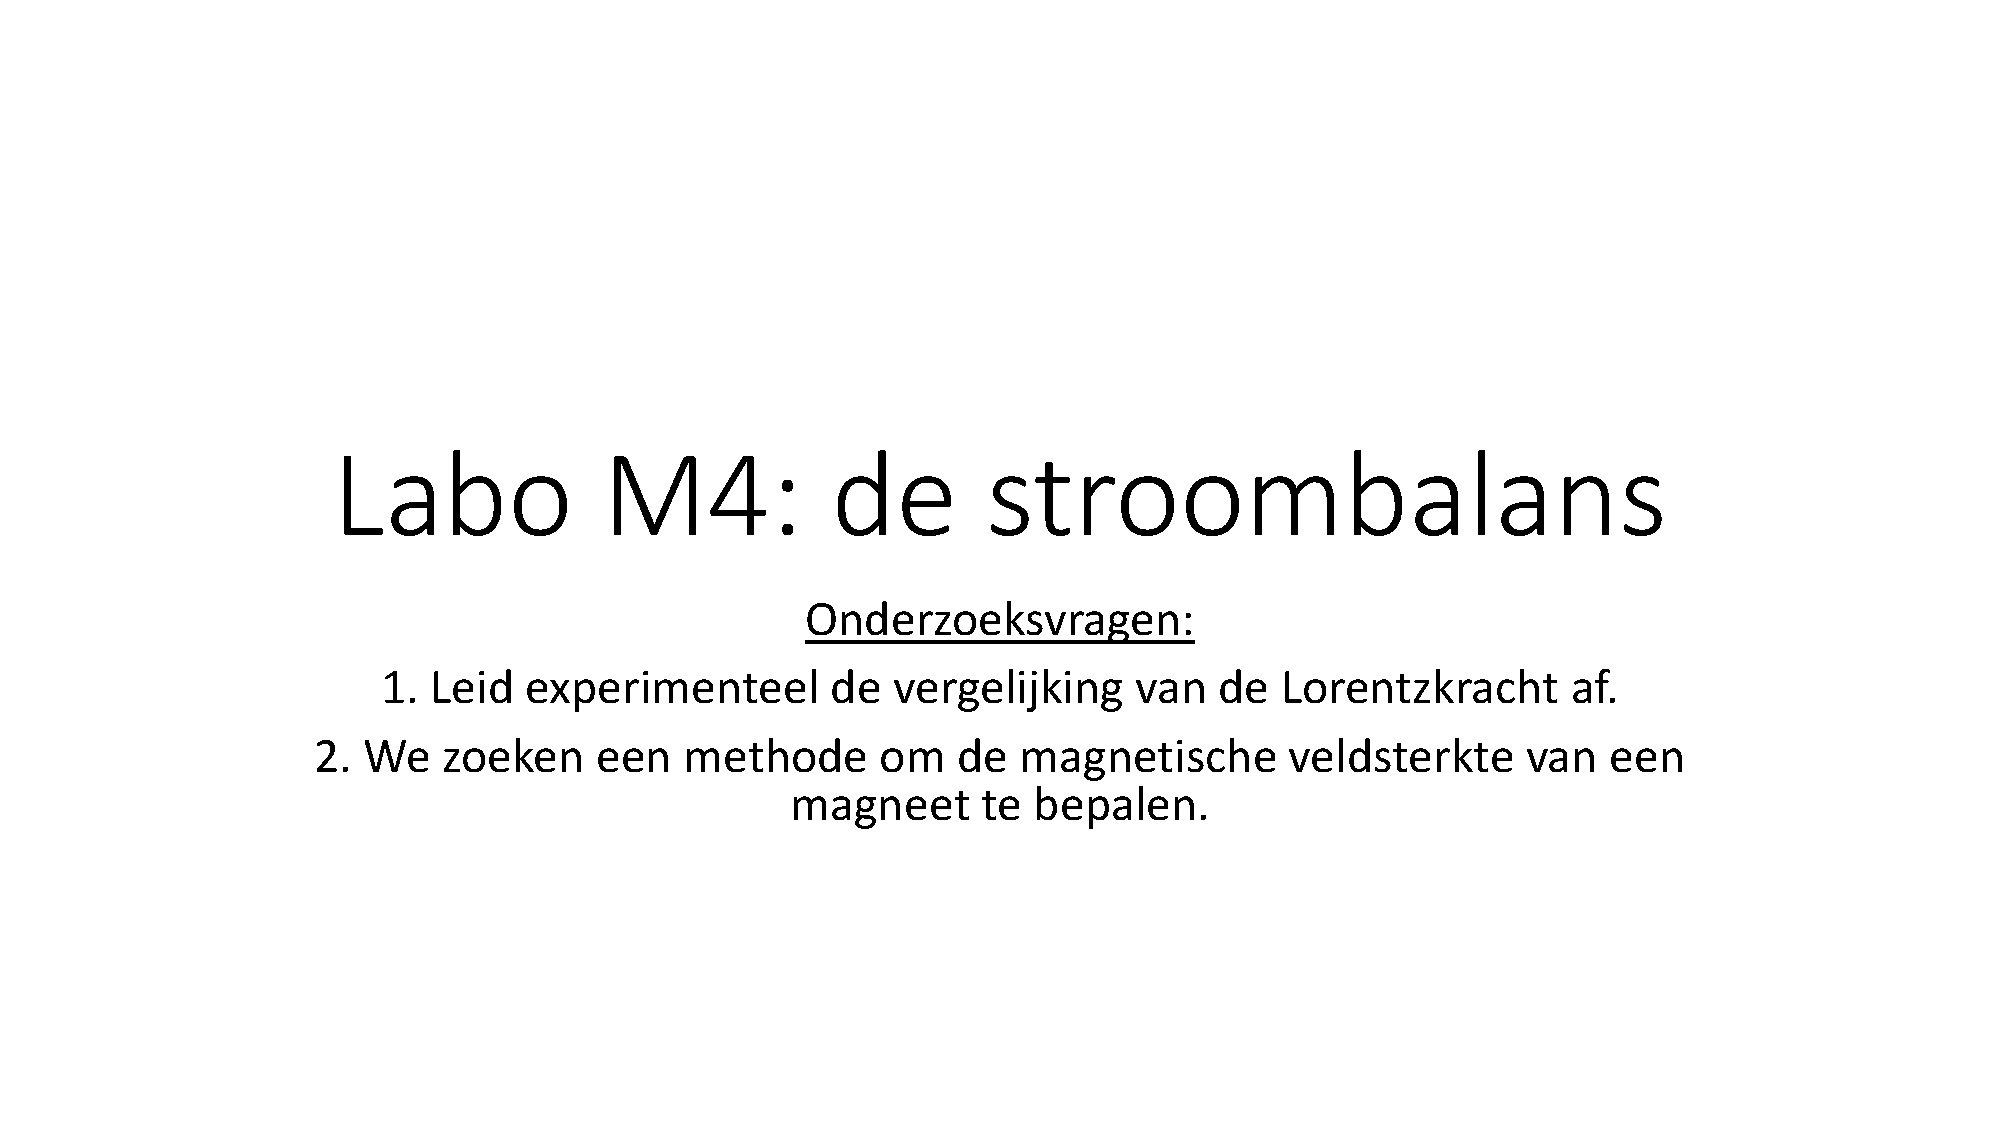
\includepdf[scale = 0.9, pages = -,pagecommand=\subsection*{Bijlage 4.2.5.1: slides},nup=2x3, delta = 0.5cm 1cm]{LaboM4.pdf}

%\subsection*{Bijlage 5.1: slides introductie}

%
%\subsection*{Bijlage 1.2: bordschema theorie}
%\begin{center}
%	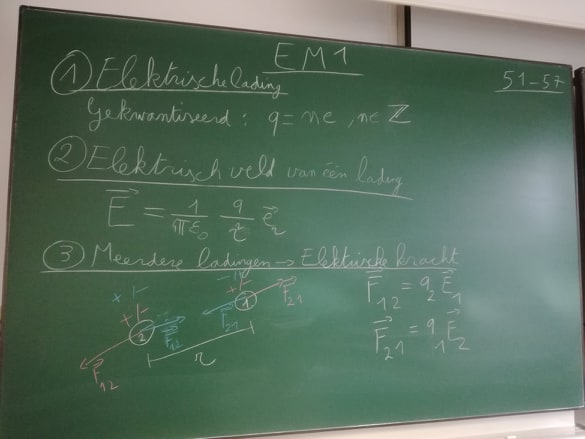
\includegraphics[width=0.9\textwidth]{Bord1a}
%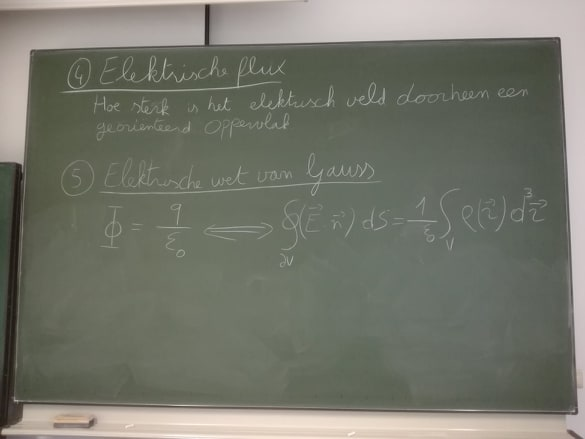
\includegraphics[width=0.9\textwidth]{Bord1b}
%\end{center}
%\newpage
%
%
%\includepdf[scale = 0.8,pages = 17,pagecommand=\subsection*{Bijlage 1.3: opgeloste oefeningen}]{Observaties_OpgelosteOef}
%\includepdf[scale = 0.8,pages =18-20,pagecommand=]{Observaties_OpgelosteOef}
%
%
%
%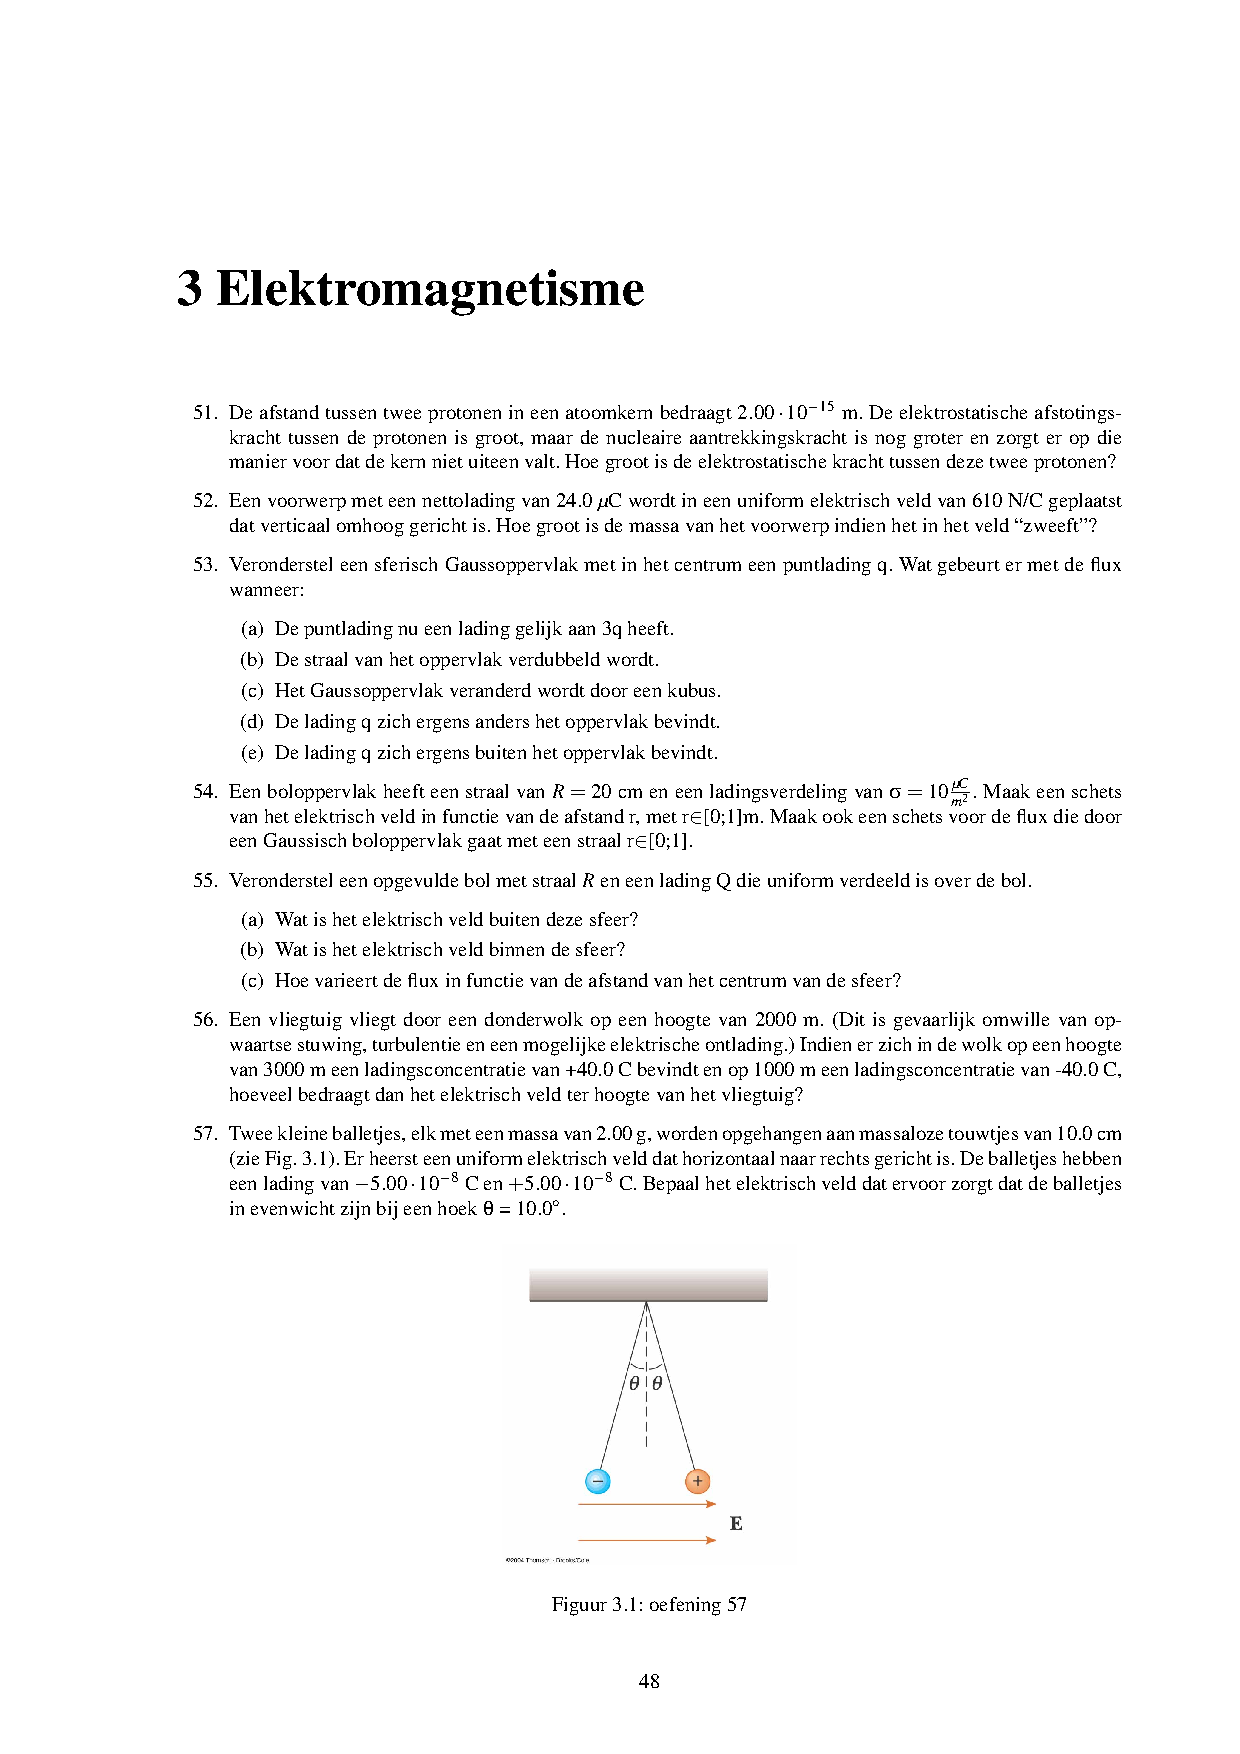
\includepdf[scale = 0.95,pages = 1,pagecommand=\subsection*{Bijlage 1.4: oefeningenbundel elektromagnetisme}]{OefeningenBundel}
%\includepdf[scale = 0.95,pages =2-,pagecommand=]{OefeningenBundel}	
% !TeX root = Stageportfolio.tex



\begin{landscape}
	Mijn stage werd vroegtijdig beëindigd vanwege de sluiting van de scholen omtrent de maatregelen die voltrokken werden vanwege Covid-19. Hieronder wil ik toch mijn reeds getroffen voorbereidingen plaatsen: de lesvoorbereiding (weliswaar met nog onvolledige beginsituatie en acties) van les 21 en het labo dat ik tijdens les 22 en 23 zou begeleiden.
	
	\subsubsection{Les 21}
	
	\begin{tabularx}{1.56\textwidth}{|p{0.35\textwidth}|X|}\hline
		\textbf{Administratieve gegevens}\newline\newline
		Kevin Truyaert\newline\newline
		technisch secundair onderwijs\newline
		3e graad, 1ste jaar, Techniek-Wetenschappen\newline
		VVKSO: \href{http://ond.vvkso-ict.com/leerplannen/doc/Toegepaste\%20fysica-2014-041.pdf}{http://ond.vvkso-ict.com/leerplannen /doc/Toegepaste\%20fysica-2014-041.pdf} \newline
		\underline{Lesonderwerp}:\newline De transformator en het elektrisch energietransport  & \textbf{Doelstellingen}
		\begin{itemize}[itemsep=0.08\baselineskip]
			\item B28: Met behulp van de wet van Lenz de zin van de inductiespanning vinden.
			\item B29: De algemene inductiewet hanteren.
			\item B31: De transformatorhouding bij de spanningen en de stromen van een ideale transformator toepassen en zijn functie bij het transport van elektrische energie toelichten.
		\end{itemize}
		\underline{Lesdoelen}\newline
		\vspace{-0.75cm}
		\begin{enumerate}[itemsep=0.08\baselineskip]
			\item De leerlingen kunnen het doel van een transformator verwoorden.
			\item De leerlingen kunnen de zin van de inductiestroom bepalen.
			\item De leerlingen kunnen de wet van Faraday-Lenz hanteren.
			\item De leerlingen kennen de transformatieverhouding voor spanningen bij een transformator.
			\item De leerlingen kennen de transformatieverhouding voor stromen bij een transformator.
			\item De leerlingen begrijpen de werking van een transformator.
			\item De leerlingen begrijpen waarom elektrische energie bij hoge spanningen vervoerd wordt. 
			\item De leerlingen kunnen het afgelegde traject tussen centrale en het stopcontact schetsen.
			\item De leerlingen kunnen de transformatieverhouding voor spanningen in oefeningen toepassen.  
			\item De leerlingen kunnen de transformatieverhouding voor stromen in oefeningen toepassen.  
		\end{enumerate} \\\hline
	\end{tabularx}\vfill \textcolor{white}{.} 


	\begin{tabularx}{1.56\textwidth}{|p{0.55\textwidth}|X|}
		\hline
		\multirow{2}{0.55\textwidth}{\textbf{Beginsituatie}\newline  
		Er zijn acht leerlingen binnen 5TW. Er heerst een algemene klassfeer. De leerlingen hebben al theorie gekregen  rond en oefeningen gemaakt op de magnetische krachtwerking. \newline\newline De leerlingen hebben vorige week de wisselspanningsgenerator gezien als een toepassing van magnetische inductie. Daarnaast kregen ze ook al een inleiding tot de transformator \newline\newline NOG AANVULLEN MET LERAARKENMERKEN.} & \textbf{Acties}\newline\newline 
		- \YellowHighlight{De transformator is een stuk fysica die in ons dagelijkse leven onbewust vaak}{15cm} \YellowHighlight{gebruikt wordt.}{3cm} Het zit in alle adapters die we gebruiken. Daarom is het belangrijk dat dit ook in de fysicales besproken wordt om de werking ervan te begrijpen.	 \newline\newline 
		\newline\newline\newline\newline\newline\newline
		
		\\ \cline{2-2}
		  & \textbf{Bronnen}\begin{itemize}
		  	\item Schramme, S. (2018) De stroombalans, labo magnetisme 4
		  	\item Frederiksen (2014), Current Balance 4565.00
		  	\item Giancoli, D. C. (2008). Physics for scientists and engineers. Pearson Education International.
		  \end{itemize}\\ \hline
	\end{tabularx}


\newpage
	
	\begin{tabularx}{1.56\textwidth}{|p{1.5cm}|p{8cm}|X|p{4cm}|}
		\hline
		\textbf{Nr. lesdoel } & \textbf{Inhoud (timing)}  & \textbf{Organisatie } & \textbf{Media } \\ \hline
		1&\underline{Herhaling wat is transformator (5 minuten)}\newline
			De leerlingen herhalen de componenten en het doel van de transformator.
		&  \underline{Onderwijsleergesprek}\newline 
			Ik schets een transformator op het bord en vraag de leerlingen wat ze van de componenten nog kunnen benoemen.
		&   Cursus hoofdstuk 6 p11\newline\newline Krijtbord \newline\newline Zelfgemaakte transfo met spoelen en weekijzeren kern staat op tafel
		\\ \hline
	\end{tabularx}\vspace{5mm}


	\begin{tabularx}{1.56\textwidth}{|p{1.5cm}|p{8cm}|X|p{4cm}|}
		\hline
		\textbf{Nr. lesdoel } & \textbf{Inhoud (timing)}  & \textbf{Organisatie } & \textbf{Media } \\ \hline
		2\newline3\newline4\newline5\newline6&\underline{Werking van de transformator (15 minuten)}\newline
		De leerlingen gebruiken de algemene inductiewet om de transformatorverhoudingen voor de spanningen en de stromen af te leiden. Door deze afleiding zullen ze ook de werking van de transformator begrijpen.
		&  \underline{Onderwijsleergesprek}\newline 
		Ik start  met het ondervragen in verband met de primaire spoel onder wisselspanning: welke fenomenen zullen er hierdoor optreden? Zo leid ik samen met de leerlingen de transformatieverhoudingen voor de spanningen en stromen af. Hierbij verwijs ik naar de tekening en naar de transfo die op tafel staat. Op die manier kunnen de leerlingen verschillende visualisaties bij dit onderwerp krijgen.
		&   Cursus hoofdstuk 6 p12\newline\newline Krijtbord \newline\newline Zelfgemaakte transfo met spoelen en weekijzeren kern staat op tafel
		\\ \hline
	\end{tabularx}\vspace{5mm}

	\begin{tabularx}{1.56\textwidth}{|p{1.5cm}|p{8cm}|X|p{4cm}|}
	\hline
	\textbf{Nr. lesdoel } & \textbf{Inhoud (timing)}  & \textbf{Organisatie } & \textbf{Media } \\ \hline
	1\newline6\newline7\newline8&\underline{Transport van elektrische} \underline{energie (15 minuten)}\newline
	Door het transport van elektrische energie te bespreken, zullen leerlingen een ander aspect van het nut van transformatoren ervaren. Ze zullen inzien dat er minder verlies is bij hoge spanningen, in vergelijking met lage spanningen. Toch kunnen we in onze leefomgeving deze hoge spanningen niet gebruiken, waardoor er transfo's gebruikt worden.
	&  \underline{Groepswerk + klassikale bespreking}\newline 
	Ik laat de leerlingen per twee aan de slag gaan om één kolom in te vullen. Daarna bespreken we klassikaal beide kolommen en besluiten de leerlingen op welke manier zij de energie zouden transporteren. Hierna bespreken we nog even kort het traject dat de energie effectief tussen centrale en klant aflegt.
	
	&   Cursus hoofdstuk 6 p13-14\newline\newline Krijtbord \newline\newline Zelfgemaakte transfo met spoelen en weekijzeren kern staat op tafel
	\\ \hline
	\end{tabularx}\vspace{5mm}

		\begin{tabularx}{1.56\textwidth}{|p{1.5cm}|p{8cm}|X|p{4cm}|}
		\hline
		\textbf{Nr. lesdoel } & \textbf{Inhoud (timing)}  & \textbf{Organisatie } & \textbf{Media } \\ \hline
		9\newline 10&\underline{Oefeningen transfo (12 minuten)}\newline
		Om voor een beter begrip van transfo's te zorgen en om een goede voorbereiding van het labo van morgen te hebben, maken we nog enkele oefeningen.
		&  \underline{Oefeningen + klassikale bespreking}\newline 
		Ik maak via onderwijsleergesprek eerst oefening 1 klassikaal. Hierna laat ik de leerlingen zelfstandig oefeningen 2 t.e.m. 5 maken. Ik probeer hier weer dat ik extra aandacht aan de minder sterke leerlingen schenk.
		&   Cursus hoofdstuk 6 p15\newline\newline Krijtbord \newline\newline Zelfgemaakte transfo met spoelen en weekijzeren kern staat op tafel
		\\ \hline
	\end{tabularx}\vspace{5mm}

\begin{tabularx}{1.56\textwidth}{|p{1.5cm}|p{8cm}|X|p{4cm}|}
	\hline
	\textbf{Nr. lesdoel } & \textbf{Inhoud (timing)}  & \textbf{Organisatie } & \textbf{Media } \\ \hline
	1&\underline{Slot (3 minuten)}\newline
	Ter voorbereiding van het labo herhaal ik nog even de kernbegrippen bij de transfo.
	&  \underline{Doceren / onderwijsleergesprek}\newline 
	Ik bespreek nog kort even de algemene werking van een transformator. Ik leg nog eens de nadruk op de transformatieverhoudingen bij ideale transfo's, maar benadruk dat ideale transfo's niet bestaan en dat ze dit morgen zullen ervaren.
	& Zelfgemaakte transfo met spoelen en weekijzeren kern staat op tafel
	\\ \hline
\end{tabularx}\vspace{5mm}


\subsubsection{Labo les 22-23}






\end{landscape}


%\subsection*{Bijlage 5.1: slides introductie}

%
%\subsection*{Bijlage 1.2: bordschema theorie}
%\begin{center}
%	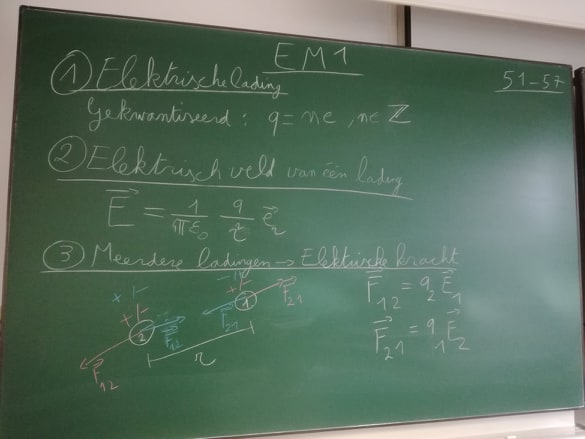
\includegraphics[width=0.9\textwidth]{Bord1a}
%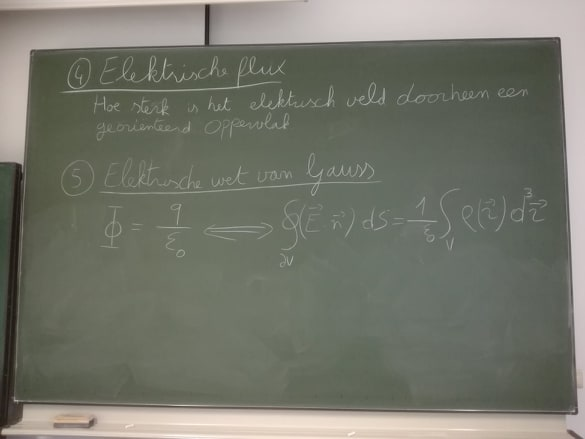
\includegraphics[width=0.9\textwidth]{Bord1b}
%\end{center}
%\newpage
%
%
%\includepdf[scale = 0.8,pages = 17,pagecommand=\subsection*{Bijlage 1.3: opgeloste oefeningen}]{Observaties_OpgelosteOef}
%\includepdf[scale = 0.8,pages =18-20,pagecommand=]{Observaties_OpgelosteOef}
%
%
%
%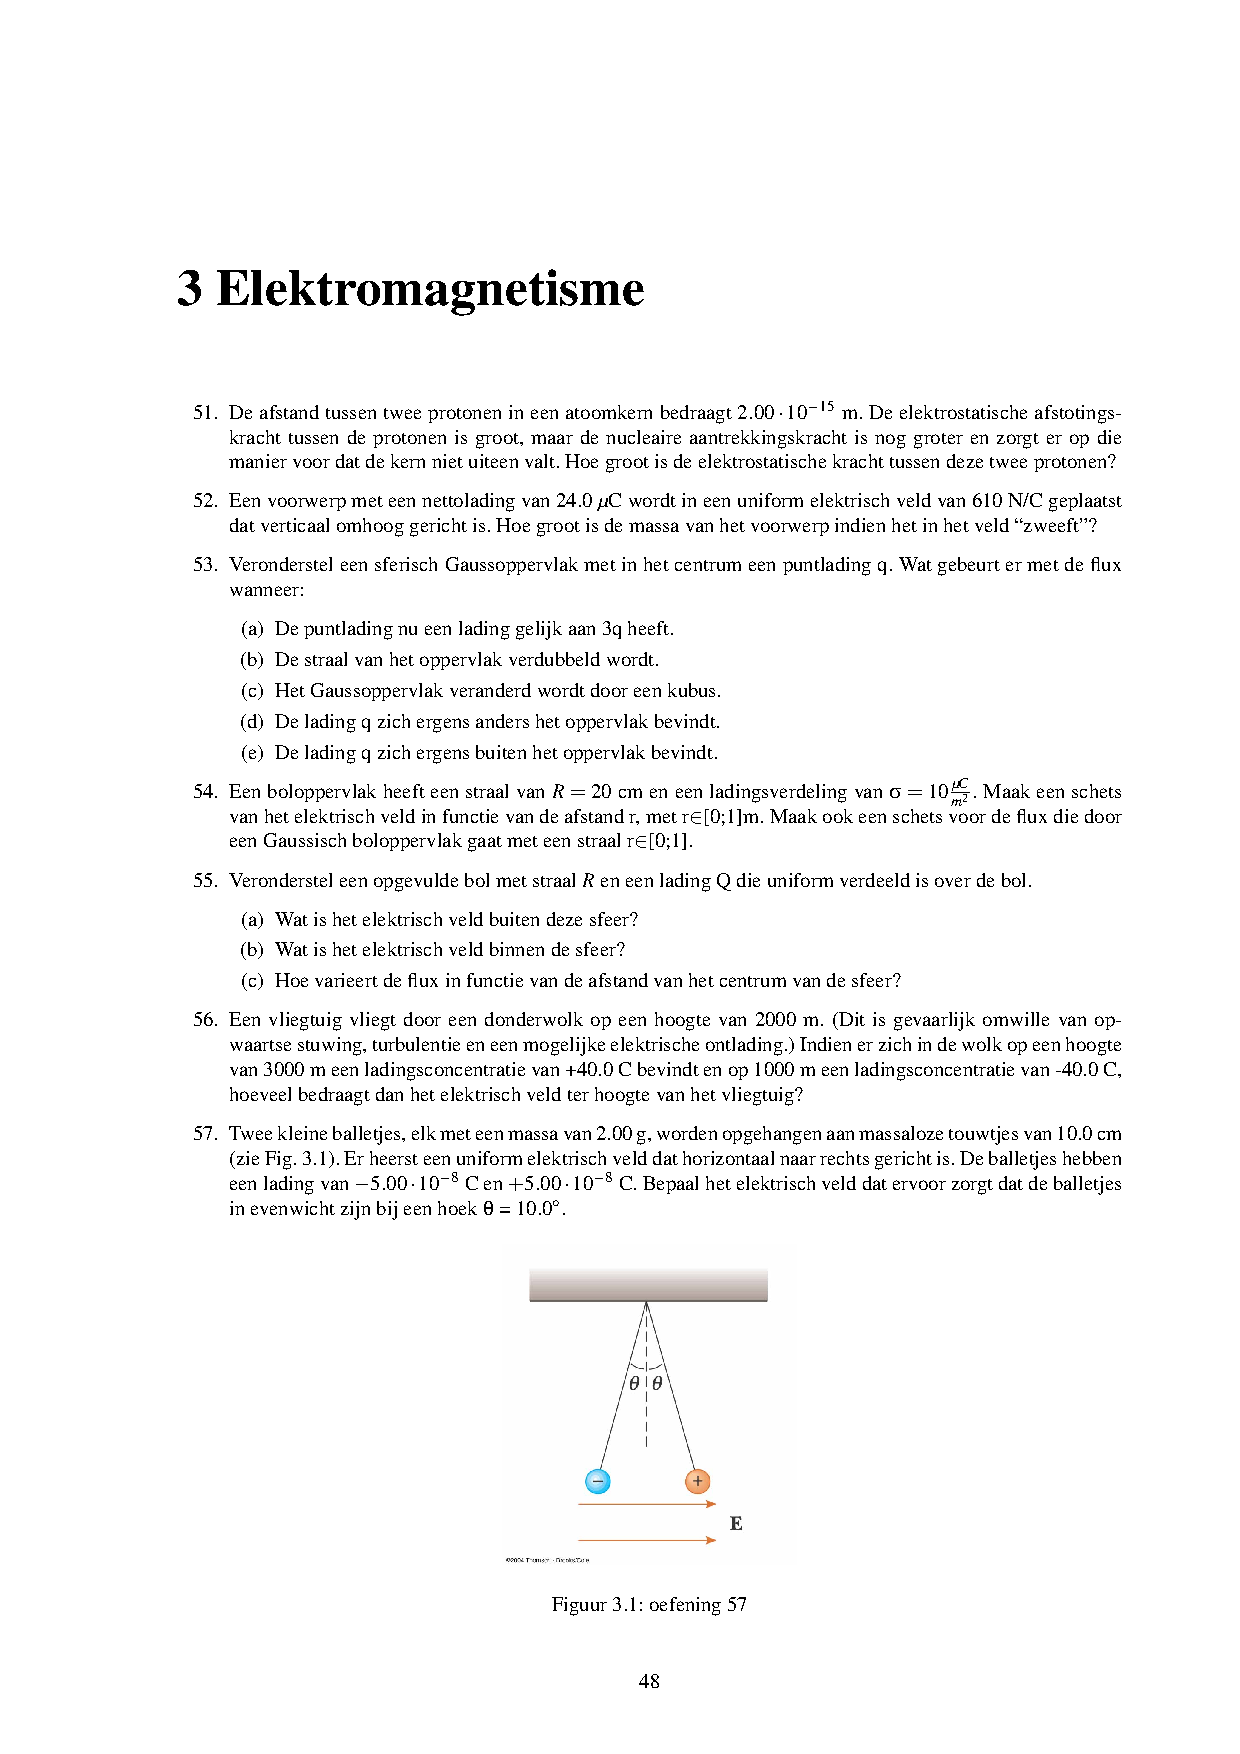
\includepdf[scale = 0.95,pages = 1,pagecommand=\subsection*{Bijlage 1.4: oefeningenbundel elektromagnetisme}]{OefeningenBundel}
%\includepdf[scale = 0.95,pages =2-,pagecommand=]{OefeningenBundel}	
	
	
	\section{Bespreking meso-activiteiten}
	Stel per meso-activiteit een verslag op op basis van volgende criteria:
	\begin{itemize}
		\item Korte situering van de drie activiteiten.
		\item Omschrijving van twee aspecten die je voor jezelf geleerd hebt uit de deelname aan de activiteiten
		\item  Toon aan met twee voorbeelden dat de activiteiten een meerwaarde zijn voor de leerkrachten.
		\item Toon aan met twee voorbeelden dat de activiteiten een meerwaarde vormen voor de leerlingen.
		\item Bespreek hoe het komt dat bepaalde activiteiten geen echte meerwaarde hebben voor leerlingen en op welke manier deze aangepast kunnen worden om toch nog functioneel te zijn voor het leerproces van de leerlingen.
	\end{itemize}
	
	\subsection{Omschrijving van de activiteiten}
	\subsubsection{Meso-activiteit 1: kinderuniversiteit Kulak}  Op zaterdag 26 oktober ging aan de katholieke universiteit campus kulak kortrijk de kinderuniversiteit door. Tijdens deze dag kunnen jongeren tussen 8 en 13 jaar ofwel de voormiddag, namiddag of hele dag op de universiteit doorbrengen. Per sessie wordt er zowel een lezing (45min) als een workshop (1u30min) aangereikt; de lezing wordt door iedereen gevolgd, waarna de jongeren zich verspreiden om per 20 à 25 een workshop te volgen.\newline
	
	
	De 15e editie van de kinderuniversiteit stond in het teken van `reis door de tijd'. De werknemers van de Kulak voorzagen tien verschillende workshops. Enkele personen binnen de fysica, waartoe ik behoor, bedachten een workshop genaamd `Bouw nu een telescoop en kijk straks naar het Universum van vroeger!'. Hiermee willen we de leerlingen bekend maken met de werking van lenzen, dat je de kleuren van de regenboog uit wit licht kan halen en dat je in het verleden kijkt wanneer je met een telescoop naar de sterren kijkt. De leerlingen krijgen tijdens de workshop eerst een halfuur uitleg van de professor door middel van een presentatie met slides en demonstratiemateriaal. Tijdens deze presentatie begint de professor met uit te leggen hoe licht werkt. Hij toont breking van licht met behulp van een laserstraal, een glazen halve cirkel (om het licht te breken) en wat krijtstof. Om reflectie duidelijk te maken, wordt er een spiegel aan de leerlingen doorgegeven. Daarna legt de prof uit hoe zowel holle als bolle lenzen werken, hoe ze ervoor zorgen dat dingen vergroot en verkleind worden en hoe je lenzen kan gebruiken om naar de ruimte te kijken. Daarna legt de professor nog uit dat het licht wel heel snel gaat, maar niet oneindig snel. Hierdoor zie je sterren zoals ze in het verleden waren. \newline\newline
	
	Na deze uitleg gaan de leerlingen aan de slag met het maken van een minitelescoop. Hiervoor gebruiken ze:
	\begin{itemize}
		\item 2 PVC-buizen met een verschillende diameter die in elkaar schuiven
		\item Twee verschillende lenzen
		\item 3D-geprinte lenshouders
		\item Plakband en versiering.
	\end{itemize}
	\begin{figure}[!h]
		\centering
		\includegraphics[width=0.9\textwidth]{Telescoop}
		\caption{Het materiaal waarmee de telescoop gemaakt wordt.}
		\label{Fig::Telescoop}
	\end{figure}
	Tijdens het maken van hun telescoop werden de leerlingen per drie meegenomen om zelf de eigenschappen van lenzen te ondervinden. Er werd een figuur op doorschijnende folie afgedrukt die een hond voorstelt en wanneer je de figuur ondersteboven houdt een kat toont. De figuur staat hieronder in beide opzichten.
	
	\begin{figure}[!b]
		\centering
		\includegraphics[width=0.5\textwidth]{HondKat}
		\caption{De figuur die gebruikt werd om de  leerlingen de eigenschappen van bolle lenzen te laten ondervinden.}
		\label{Fig::HondKat}
	\end{figure}
	Door middel van een opstelling met bolle lenzen is het mogelijk om beide figuren zichtbaar te maken, aangezien bolle lenzen het beeld kunnen omdraaien. De opstelling werd aan de leerlingen voorgesteld en iedere component werd benoemd. Door aan de  leerlingen de vraag te stellen hoe het mogelijk is dat beide beelden uit het ene beeld voortkomen wisten er sommigen de eigenschappen van bolle lenzen, die ze net gehoord hadden, te gebruiken om dit te verklaren. 
	
	Wanneer alle jongeren hun telescoop gemaakt hebben, kunnen ze op zoek gaan naar hun naam die op een ster geschreven staat. Die sterren hangen een eindje verder, waardoor hun namen niet zichtbaar zijn met het blote oog, maar wel met de gemaakte telescoop. 
	
	\subsection{Twee aspecten die ik voor mezelf geleerd heb}
	
	\subsection{Twee voorbeelden die aantonen dat de activiteiten een meerwaarde zijn voor leerkrachten}
	\begin{itemize}[labelwidth=3em,leftmargin =\dimexpr\labelwidth+\labelsep\relax]
		\item[Meso 1] Ondanks dat de werking van lenzen geen makkelijke materie is, was ik verbaasd van de interpretatie van sommige jongeren bij de proef met de hond-kat. In eerste instantie vonden ze het heel vreemd wat er aan de hand was: ze zagen twee verschillende beelden, maar die kwamen allebei van dezelfde foto. Door als leerkracht hier gerichte vragen te stellen, kun je de leerlingen zelfontdekkend laten leren. Het zijn zijzelf die de link leggen tussen de eigenschappen van lenzen: bolle lenzen draaien je beeld om en maken het reëel, terwijl holle lenzen de oriëntatie van het beeld behouden, maar dat het beeld virtueel wordt. Hierdoor wordt mijn beeld van zelfontdekkend leren  binnen het juiste tijdskader versterkt.
	\end{itemize}
	
	\subsection{Twee voorbeelden die aantonen dat de activiteiten een meerwaarde zijn voor leerlingen}
	
	
	\subsection{Voorbeelden die geen echte meerwaarde hebben voor de  leerlingen en op welke manier deze aangepast kunnen worden om toch nog functioneel te zijn voor het leerproces van de leerlingen}
	
	
	
	
	
	
	\section{Evaluatiedocumenten vakmentor}
	
	\includepdf[scale = 0.8,pages = 3,pagecommand=\subsection{Evaluatiedocumenten mentor Kulak (LIO): eerste geobserveerde les}]{VerslagenDavid2}
	\includepdf[scale = 0.8,pages =4-5,pagecommand=]{VerslagenDavid2}
	
	
	\includepdf[scale = 0.8,pages = 7,pagecommand=\subsection{Evaluatiedocumenten mentor Kulak (LIO): tweede geobserveerde les}]{VerslagenDavid}
	\includepdf[scale = 0.8,pages =8-9,pagecommand=]{VerslagenDavid2}
	
	
	
	\includepdf[scale = 0.8,pages = 10,pagecommand=\subsection{Eindevaluatiedocument mentor Kulak (LIO)}]{VerslagenDavid2}

	
	
	
	\section{Evaluatiedocument klasbezoek stagebegeleider}
	
	\section{Eindreflectie}
	Stel een eindreflectie op waarin je volgende aspecten behandelt: 
	
	1) Waren er factoren die bevorderend of belemmerend werkten m.b.t. het goed doorlopen van je stage? 
	2) Waarvoor had je graag bijkomende begeleiding gekregen van je vakmentoren? 
	3) Waarvoor had je graag bijkomende begeleiding gekregen van je stagebegeleider? 
	4) Bekijk aandachtig de acties die je in het begin van je stage opstelde in jouw POP . Ga na of je via de acties jouw leerdoelen hebt behaald. Verwijs heel duidelijk naar informatie in je portfolio waar en hoe je deze acties aan bod liet komen. 
	5)  Bestudeer nogmaals het opleidingsprofiel en de basiscompetenties van een leraar (link):  bespreek minstens 5 basiscompetenties die je succesvol hebt behaald tijdens het uitvoeren van je stage. 
	Jouw eindreflectie is maximaal drie A4-pagina’s lang. 
	
	
	
	\section{Voorbereiding eindassessment}
	
	Om het eindassessment voor te bereiden, kan je gebruik maken van volgende vragen:
	• Lees jouw eindreflectie goed na en bekijk jouw leerdoelen en uitgewerkte acties. Recapituleer hoe je de stage hebt ervaren. Waarom moet een directeur jou als leerkracht aanwerven? Wat heb jij een schoolteam te bieden? Waar zie je nog uitdagingen voor jezelf? 
	• Waar heb je nog aanvangsbegeleiding nodig en wie kan jou daarbij helpen (toon je inzicht in vakgroep- en schoolwerking aan)?
	• Hoe heb je de lerarenopleiding in het algemeen ervaren? Wat vond je positief? Wat heb je gemist tijdens de opleiding? 
	
	
	
	
	
	
\end{document}
